%% Phase 4 final research paper -- IEEE journal format (class IEEEtran), two-column.
%% Written by hand from the reviewed _v2 manuscript (PHASE4_RESEARCH_PAPER_v2.tex), restructured to the Phase 4
%% section order and length; see MANUSCRIPT_REVISION_LOG.md. Every result is a \V{key} macro from
%% generated/numbers_v2.tex (built by build/build_numbers_v2.py from committed result files; map in
%% NUMBERS_MAP_v2.csv). Extended material is in PHASE4_FINAL_SUPPLEMENT.tex (labels prefixed S- below).
%% Build (from phase4_v2/): see README.md, section "Final paper".
\input{glyphtounicode}\pdfgentounicode=1
\documentclass[journal]{IEEEtran}

\usepackage{graphicx}%
\usepackage{multirow}%
\usepackage{amsmath,amssymb,amsfonts}%
\usepackage{xcolor}%
\usepackage{textcomp}%
\usepackage{booktabs}%
\usepackage{algorithm}%
\usepackage{algorithmicx}%
\usepackage{algpseudocode}%
\usepackage{tabularx}%
\usepackage{array}%
\usepackage{url}%
\usepackage{xr-hyper}%
\externaldocument[S-]{PHASE4_FINAL_SUPPLEMENT_labels}
\usepackage[hidelinks]{hyperref}
\newcolumntype{Y}{>{\raggedright\arraybackslash}X}

% generated by scripts/paper/build_numbers_v2.py -- do not edit; every value is in docs/paper/NUMBERS_MAP_v2.csv
\makeatletter
\expandafter\def\csname V@abl:A1|S1-DEB|S1:ci95\endcsname{[\textminus{}0.074, 0.105]}
\expandafter\def\csname V@abl:A1|S1-DEB|S1:delta\endcsname{+0.016}
\expandafter\def\csname V@abl:A1|S1-DEB|S1:p\endcsname{0.731}
\expandafter\def\csname V@abl:A2|S1-DEB|S1:ci95\endcsname{[\textminus{}0.039, 0.141]}
\expandafter\def\csname V@abl:A2|S1-DEB|S1:delta\endcsname{+0.051}
\expandafter\def\csname V@abl:A2|S1-DEB|S1:p\endcsname{0.266}
\expandafter\def\csname V@abl:DEB|S1|impl-DEB|S1:ci95\endcsname{[\textminus{}0.214, 0.045]}
\expandafter\def\csname V@abl:DEB|S1|impl-DEB|S1:delta\endcsname{\textminus{}0.086}
\expandafter\def\csname V@abl:DEB|S1|impl-DEB|S1:p\endcsname{0.193}
\expandafter\def\csname V@abl:DEB|S1|noF-DEB|S1:ci95\endcsname{[\textminus{}0.282, 0.034]}
\expandafter\def\csname V@abl:DEB|S1|noF-DEB|S1:delta\endcsname{\textminus{}0.122}
\expandafter\def\csname V@abl:DEB|S1|noF-DEB|S1:p\endcsname{0.136}
\expandafter\def\csname V@abl:J1|S1|impl-J1|S1:ci95\endcsname{[\textminus{}0.053, 0.122]}
\expandafter\def\csname V@abl:J1|S1|impl-J1|S1:delta\endcsname{+0.036}
\expandafter\def\csname V@abl:J1|S1|impl-J1|S1:p\endcsname{0.406}
\expandafter\def\csname V@abl:J1|S1|noF-J1|S1:ci95\endcsname{[\textminus{}0.314, \textminus{}0.006]}
\expandafter\def\csname V@abl:J1|S1|noF-J1|S1:delta\endcsname{\textminus{}0.163}
\expandafter\def\csname V@abl:J1|S1|noF-J1|S1:p\endcsname{0.042}
\expandafter\def\csname V@abl:J1|S2|specprime-J1|S2:ci95\endcsname{[\textminus{}0.040, 0.132]}
\expandafter\def\csname V@abl:J1|S2|specprime-J1|S2:delta\endcsname{+0.042}
\expandafter\def\csname V@abl:J1|S2|specprime-J1|S2:p\endcsname{0.330}
\expandafter\def\csname V@abl:SC|S1|noF-SC|S1:ci95\endcsname{[\textminus{}0.490, \textminus{}0.083]}
\expandafter\def\csname V@abl:SC|S1|noF-SC|S1:delta\endcsname{\textminus{}0.282}
\expandafter\def\csname V@abl:SC|S1|noF-SC|S1:p\endcsname{0.003}
\expandafter\def\csname V@arow:few all\endcsname{125}
\expandafter\def\csname V@arow:few pf\endcsname{21}
\expandafter\def\csname V@arow:few tf\endcsname{104}
\expandafter\def\csname V@arow:jackson dec tf\endcsname{117}
\expandafter\def\csname V@arow:jackson pf\endcsname{8}
\expandafter\def\csname V@arow:jackson tf\endcsname{229}
\expandafter\def\csname V@arow:lang57 pf\endcsname{13}
\expandafter\def\csname V@arow:math59 ncomp\endcsname{10}
\expandafter\def\csname V@atx:a6 mismatches\endcsname{0}
\expandafter\def\csname V@atx:a6 records\endcsname{834}
\expandafter\def\csname V@atx:a7 sources\endcsname{15}
\expandafter\def\csname V@atx:a8 pass\endcsname{9}
\expandafter\def\csname V@atx:auroc flip\endcsname{0.526}
\expandafter\def\csname V@atx:auroc votes\endcsname{0.772}
\expandafter\def\csname V@atx:auroc votes dec\endcsname{0.787}
\expandafter\def\csname V@atx:dec unanimous\endcsname{77}
\expandafter\def\csname V@atx:elig ci\endcsname{[0.130, 0.462]}
\expandafter\def\csname V@atx:elig est@signed\endcsname{+0.297}
\expandafter\def\csname V@atx:frame bugs\endcsname{322}
\expandafter\def\csname V@atx:ft focal pf\endcsname{21}
\expandafter\def\csname V@atx:ft focal pfdec\endcsname{0}
\expandafter\def\csname V@atx:ft focal tf\endcsname{58}
\expandafter\def\csname V@atx:ft focal tfdec\endcsname{11}
\expandafter\def\csname V@atx:ft main pf\endcsname{6}
\expandafter\def\csname V@atx:ft main pfdec\endcsname{0}
\expandafter\def\csname V@atx:ft main tf\endcsname{67}
\expandafter\def\csname V@atx:ft main tfdec\endcsname{41}
\expandafter\def\csname V@atx:ft test pf\endcsname{0}
\expandafter\def\csname V@atx:ft test pfdec\endcsname{0}
\expandafter\def\csname V@atx:ft test tf\endcsname{93}
\expandafter\def\csname V@atx:ft test tfdec\endcsname{41}
\expandafter\def\csname V@atx:het ci\endcsname{[0.089, 0.469]}
\expandafter\def\csname V@atx:jk c1 ci\endcsname{[\textminus{}0.199, 0.255]}
\expandafter\def\csname V@atx:jk c2 ci\endcsname{[0.109, 0.377]}
\expandafter\def\csname V@atx:labels recomputed\endcsname{834}
\expandafter\def\csname V@atx:mh@signed\endcsname{+0.149}
\expandafter\def\csname V@atx:minshield pf\endcsname{19}
\expandafter\def\csname V@atx:minshield tf\endcsname{83}
\expandafter\def\csname V@atx:noJ ci\endcsname{[\textminus{}0.035, 0.108]}
\expandafter\def\csname V@atx:noJ est@signed\endcsname{+0.041}
\expandafter\def\csname V@atx:noJ n\endcsname{335}
\expandafter\def\csname V@atx:noJDB ci\endcsname{[\textminus{}0.007, 0.204]}
\expandafter\def\csname V@atx:orig bugs\endcsname{92}
\expandafter\def\csname V@atx:pilot chart flip\endcsname{20}
\expandafter\def\csname V@atx:pilot chart pf\endcsname{20}
\expandafter\def\csname V@atx:pilot math flip\endcsname{0}
\expandafter\def\csname V@atx:pilot math pf\endcsname{11}
\expandafter\def\csname V@atx:plan hi\endcsname{50}
\expandafter\def\csname V@atx:plan lo\endcsname{30}
\expandafter\def\csname V@atx:projboot ci\endcsname{[0.032, 0.426]}
\expandafter\def\csname V@atx:projboot n\endcsname{12}
\expandafter\def\csname V@atx:seed sd f1@3\endcsname{0.007}
\expandafter\def\csname V@atx:seed sd f2@3\endcsname{0.006}
\expandafter\def\csname V@atx:stack pf\endcsname{6}
\expandafter\def\csname V@atx:stack tf\endcsname{160}
\expandafter\def\csname V@atx:t analysis\endcsname{09:09:50}
\expandafter\def\csname V@atx:t labels\endcsname{07:09:02}
\expandafter\def\csname V@atx:t ledger\endcsname{07:52:40}
\expandafter\def\csname V@atx:t probe\endcsname{07:10:05}
\expandafter\def\csname V@atx:t vote\endcsname{07:53:41}
\expandafter\def\csname V@atx:top bugs dec\endcsname{92}
\expandafter\def\csname V@atx:top bugs n\endcsname{6}
\expandafter\def\csname V@aud2:consensus_vs_execution:agreement@pct1\endcsname{97.2\%}
\expandafter\def\csname V@aud2:consensus_vs_execution:kappa_pf_tf\endcsname{0.934}
\expandafter\def\csname V@aud2:llm_rater_secondary_D84:consensus_vs_C:kappa\endcsname{0.903}
\expandafter\def\csname V@aud2:raters:kappa\endcsname{0.936}
\expandafter\def\csname V@aud2:raters:kappa_ci95_bug_bootstrap\endcsname{[0.638, 1.000]}
\expandafter\def\csname V@aud:dev_split_labels:TF\endcsname{89}
\expandafter\def\csname V@aud:labels:PF\endcsname{21}
\expandafter\def\csname V@aud:labels:TF\endcsname{50}
\expandafter\def\csname V@aud:n_items\endcsname{71}
\expandafter\def\csname V@cas1:escalation:share_escalated@pct0\endcsname{61\%}
\expandafter\def\csname V@cas1:summary:CAS|S1:f1\endcsname{0.741}
\expandafter\def\csname V@cas1:summary:CAS|S1:mcc\endcsname{0.595}
\expandafter\def\csname V@cas1:summary:CAS|S1:pf_lost@1\endcsname{10.3}
\expandafter\def\csname V@cas2:escalation:escalated@0\endcsname{134}
\expandafter\def\csname V@cas2:escalation:frontier_calls_all_per_replicate@0\endcsname{1,350}
\expandafter\def\csname V@cas2:escalation:frontier_calls_cascade_per_replicate@0\endcsname{670}
\expandafter\def\csname V@cas2:escalation:share_escalated@pct0\endcsname{50\%}
\expandafter\def\csname V@cas2:escalation:share_escalated@pct1\endcsname{49.6\%}
\expandafter\def\csname V@cas2:escalation:tier1_discard@0\endcsname{35}
\expandafter\def\csname V@cas2:escalation:tier1_keep@0\endcsname{101}
\expandafter\def\csname V@cas2:hypotheses:H12-1:ci95\endcsname{[0.202, 0.460]}
\expandafter\def\csname V@cas2:hypotheses:H12-1:delta\endcsname{+0.311}
\expandafter\def\csname V@cas2:hypotheses:H12-1:p_holm\endcsname{\textless{}0.001}
\expandafter\def\csname V@cas2:hypotheses:H12-2:ci90\endcsname{[\textminus{}0.075, \textminus{}0.022]}
\expandafter\def\csname V@cas2:hypotheses:H12-2:ci95\endcsname{[\textminus{}0.081, \textminus{}0.018]}
\expandafter\def\csname V@cas2:hypotheses:H12-2:delta\endcsname{\textminus{}0.046}
\expandafter\def\csname V@cas2:hypotheses:H12-2:p_holm\endcsname{0.397}
\expandafter\def\csname V@cas2:n_bugs\endcsname{64}
\expandafter\def\csname V@cas2:n_instances\endcsname{270}
\expandafter\def\csname V@cas2:summary:CASJ1|S1:f1\endcsname{0.833}
\expandafter\def\csname V@cas2:summary:CASJ1|S1:mcc\endcsname{0.606}
\expandafter\def\csname V@cas2:summary:CASJ1|S1:pf_lost@0\endcsname{24}
\expandafter\def\csname V@cas2:summary:CASJ1|S1:precision\endcsname{0.823}
\expandafter\def\csname V@cas2:summary:CASJ1|S1:recall\endcsname{0.844}
\expandafter\def\csname V@cas2:summary:CAS|S1:f1\endcsname{0.863}
\expandafter\def\csname V@cas2:summary:CAS|S1:mcc\endcsname{0.666}
\expandafter\def\csname V@cas2:summary:CAS|S1:pf_lost@0\endcsname{15}
\expandafter\def\csname V@cas2:summary:CAS|S1:precision\endcsname{0.827}
\expandafter\def\csname V@cas2:summary:CAS|S1:recall\endcsname{0.903}
\expandafter\def\csname V@cas2:summary:DEB|S1:f1\endcsname{0.700}
\expandafter\def\csname V@cas2:summary:DEB|S1:mcc\endcsname{0.392}
\expandafter\def\csname V@cas2:summary:DEB|S1:pf_lost@0\endcsname{56}
\expandafter\def\csname V@cas2:summary:DEB|S1:precision\endcsname{0.778}
\expandafter\def\csname V@cas2:summary:DEB|S1:recall\endcsname{0.636}
\expandafter\def\csname V@cas2:summary:DEB|S1|SON:f1\endcsname{0.910}
\expandafter\def\csname V@cas2:summary:DEB|S1|SON:mcc\endcsname{0.788}
\expandafter\def\csname V@cas2:summary:DEB|S1|SON:pf_lost@0\endcsname{13}
\expandafter\def\csname V@cas2:summary:DEB|S1|SON:precision\endcsname{0.904}
\expandafter\def\csname V@cas2:summary:DEB|S1|SON:recall\endcsname{0.916}
\expandafter\def\csname V@cas2:summary:J1|S1|SON:f1\endcsname{0.845}
\expandafter\def\csname V@cas2:summary:J1|S1|SON:mcc\endcsname{0.687}
\expandafter\def\csname V@cas2:summary:J1|S1|SON:pf_lost@0\endcsname{34}
\expandafter\def\csname V@cas2:summary:J1|S1|SON:precision\endcsname{0.923}
\expandafter\def\csname V@cas2:summary:J1|S1|SON:recall\endcsname{0.779}
\expandafter\def\csname V@cas2:summary:KUU|S1:f1\endcsname{0.771}
\expandafter\def\csname V@cas2:summary:KUU|S1:mcc\endcsname{0.356}
\expandafter\def\csname V@cas2:summary:KUU|S1:pf_lost@0\endcsname{4}
\expandafter\def\csname V@cas2:summary:KUU|S1:precision\endcsname{0.638}
\expandafter\def\csname V@cas2:summary:KUU|S1:recall\endcsname{0.974}
\expandafter\def\csname V@cc:control:PF\endcsname{0}
\expandafter\def\csname V@cc:control:bugs\endcsname{59}
\expandafter\def\csname V@cc:control:decoupled_rate_TF@3\endcsname{0.187}
\expandafter\def\csname V@cc:control:flip_rate_PF_in_F1F2@3\endcsname{0.255}
\expandafter\def\csname V@cc:control:flip_rate_TF@3\endcsname{0.220}
\expandafter\def\csname V@cc:control:flip_rate_TF_ci95\endcsname{[0.137, 0.321]}
\expandafter\def\csname V@cc:control:flip_rate_TF_in_F1F2@3\endcsname{0.226}
\expandafter\def\csname V@cc:control:instances\endcsname{246}
\expandafter\def\csname V@cc:family:C1:PF\endcsname{55}
\expandafter\def\csname V@cc:family:C1:PF_flagged\endcsname{14}
\expandafter\def\csname V@cc:family:C1:TF\endcsname{517}
\expandafter\def\csname V@cc:family:C1:TF_flagged\endcsname{117}
\expandafter\def\csname V@cc:family:C1:ci95\endcsname{[\textminus{}0.137, 0.274]}
\expandafter\def\csname V@cc:family:C1:difference@signed\endcsname{+0.028}
\expandafter\def\csname V@cc:family:C1:p@4\endcsname{0.7685}
\expandafter\def\csname V@cc:family:C1:p_holm@4\endcsname{1.0000}
\expandafter\def\csname V@cc:family:C2:PF\endcsname{55}
\expandafter\def\csname V@cc:family:C2:PF_flagged\endcsname{1}
\expandafter\def\csname V@cc:family:C2:TF\endcsname{517}
\expandafter\def\csname V@cc:family:C2:TF_flagged\endcsname{135}
\expandafter\def\csname V@cc:family:C2:ci95\endcsname{[0.114, 0.372]}
\expandafter\def\csname V@cc:family:C2:difference@signed\endcsname{+0.243}
\expandafter\def\csname V@cc:family:C2:p@4\endcsname{0.0006}
\expandafter\def\csname V@cc:family:C2:p_holm@4\endcsname{0.0024}
\expandafter\def\csname V@cc:family:C3:ci95\endcsname{[0.001, 0.099]}
\expandafter\def\csname V@cc:family:C3:difference@signed\endcsname{+0.048}
\expandafter\def\csname V@cc:family:C3:p@4\endcsname{0.0474}
\expandafter\def\csname V@cc:family:C3:p_holm@4\endcsname{0.1422}
\expandafter\def\csname V@cc:family:C4:ci95\endcsname{[\textminus{}3.000, 0.000]}
\expandafter\def\csname V@cc:family:C4:difference@signed\endcsname{\textminus{}1.000}
\expandafter\def\csname V@cc:family:C4:p@4\endcsname{0.7375}
\expandafter\def\csname V@cc:family:C4:p_holm@4\endcsname{1.0000}
\expandafter\def\csname V@cc:population:PF\endcsname{55}
\expandafter\def\csname V@cc:population:TF\endcsname{517}
\expandafter\def\csname V@cc:population:bugs\endcsname{104}
\expandafter\def\csname V@cc:population:bugs_with_PF\endcsname{21}
\expandafter\def\csname V@cc:population:instances\endcsname{572}
\expandafter\def\csname V@cc:resamples\endcsname{10,000}
\expandafter\def\csname V@cc:rules:2-of-3+CK+CD:BA@3\endcsname{0.717}
\expandafter\def\csname V@cc:rules:2-of-3+CK+CD:PF_lost\endcsname{7}
\expandafter\def\csname V@cc:rules:2-of-3+CK+CD:TNR@3\endcsname{0.564}
\expandafter\def\csname V@cc:rules:2-of-3+CK+CD:TPR@3\endcsname{0.870}
\expandafter\def\csname V@cc:rules:2-of-3+CK+CD:bugs_lost\endcsname{4}
\expandafter\def\csname V@cc:rules:2-of-3+CK+CD:bugs_with_PF\endcsname{21}
\expandafter\def\csname V@cc:rules:2-of-3+CK+CD:upper95_bug_loss_rate@3\endcsname{0.384}
\expandafter\def\csname V@cc:rules:2-of-3+CK:BA@3\endcsname{0.695}
\expandafter\def\csname V@cc:rules:2-of-3+CK:PF_lost\endcsname{6}
\expandafter\def\csname V@cc:rules:2-of-3+CK:TNR@3\endcsname{0.501}
\expandafter\def\csname V@cc:rules:2-of-3+CK:TPR@3\endcsname{0.889}
\expandafter\def\csname V@cc:rules:2-of-3+CK:bugs_lost\endcsname{3}
\expandafter\def\csname V@cc:rules:2-of-3+CK:bugs_with_PF\endcsname{21}
\expandafter\def\csname V@cc:rules:2-of-3+CK:upper95_bug_loss_rate@3\endcsname{0.329}
\expandafter\def\csname V@cc:rules:2-of-3:BA@3\endcsname{0.696}
\expandafter\def\csname V@cc:rules:2-of-3:PF_lost\endcsname{7}
\expandafter\def\csname V@cc:rules:2-of-3:TNR@3\endcsname{0.521}
\expandafter\def\csname V@cc:rules:2-of-3:TPR@3\endcsname{0.870}
\expandafter\def\csname V@cc:rules:2-of-3:bugs_lost\endcsname{4}
\expandafter\def\csname V@cc:rules:2-of-3:bugs_with_PF\endcsname{21}
\expandafter\def\csname V@cc:rules:2-of-3:upper95_bug_loss_rate@3\endcsname{0.384}
\expandafter\def\csname V@cc:rules:KUU+CD:BA@3\endcsname{0.706}
\expandafter\def\csname V@cc:rules:KUU+CD:PF_lost\endcsname{1}
\expandafter\def\csname V@cc:rules:KUU+CD:TNR@3\endcsname{0.430}
\expandafter\def\csname V@cc:rules:KUU+CD:TPR@3\endcsname{0.982}
\expandafter\def\csname V@cc:rules:KUU+CD:bugs_lost\endcsname{1}
\expandafter\def\csname V@cc:rules:KUU+CD:bugs_with_PF\endcsname{21}
\expandafter\def\csname V@cc:rules:KUU+CD:upper95_bug_loss_rate@3\endcsname{0.207}
\expandafter\def\csname V@cc:rules:KUU+CK+CD:BA@3\endcsname{0.701}
\expandafter\def\csname V@cc:rules:KUU+CK+CD:PF_lost\endcsname{1}
\expandafter\def\csname V@cc:rules:KUU+CK+CD:TNR@3\endcsname{0.420}
\expandafter\def\csname V@cc:rules:KUU+CK+CD:TPR@3\endcsname{0.982}
\expandafter\def\csname V@cc:rules:KUU+CK+CD:bugs_lost\endcsname{1}
\expandafter\def\csname V@cc:rules:KUU+CK+CD:bugs_with_PF\endcsname{21}
\expandafter\def\csname V@cc:rules:KUU+CK+CD:upper95_bug_loss_rate@3\endcsname{0.207}
\expandafter\def\csname V@cc:rules:KUU:BA@3\endcsname{0.658}
\expandafter\def\csname V@cc:rules:KUU:PF_lost\endcsname{0}
\expandafter\def\csname V@cc:rules:KUU:TNR@3\endcsname{0.316}
\expandafter\def\csname V@cc:rules:KUU:TPR@3\endcsname{1.000}
\expandafter\def\csname V@cc:rules:KUU:bugs_lost\endcsname{0}
\expandafter\def\csname V@cc:rules:KUU:bugs_with_PF\endcsname{21}
\expandafter\def\csname V@cc:rules:KUU:upper95_bug_loss_rate@3\endcsname{0.133}
\expandafter\def\csname V@cc:rules:PF\endcsname{54}
\expandafter\def\csname V@cc:rules:instances_with_three_votes\endcsname{561}
\expandafter\def\csname V@cc:rules:keep-all+CD:BA@3\endcsname{0.624}
\expandafter\def\csname V@cc:rules:keep-all+CD:PF_lost\endcsname{1}
\expandafter\def\csname V@cc:rules:keep-all+CD:TNR@3\endcsname{0.266}
\expandafter\def\csname V@cc:rules:keep-all+CD:TPR@3\endcsname{0.982}
\expandafter\def\csname V@cc:rules:keep-all+CD:bugs_lost\endcsname{1}
\expandafter\def\csname V@cc:rules:keep-all+CD:bugs_with_PF\endcsname{21}
\expandafter\def\csname V@cc:rules:keep-all+CD:upper95_bug_loss_rate@3\endcsname{0.207}
\expandafter\def\csname V@cc:secondary:clean_operator_flip:PF_flagged\endcsname{13}
\expandafter\def\csname V@cc:secondary:clean_operator_flip:TF_flagged\endcsname{95}
\expandafter\def\csname V@cc:secondary:clean_operator_flip:ci95\endcsname{[\textminus{}0.112, 0.294]}
\expandafter\def\csname V@cc:secondary:clean_operator_flip:difference@signed\endcsname{+0.053}
\expandafter\def\csname V@cc:secondary:focal_body_only_flip:PF_flagged\endcsname{12}
\expandafter\def\csname V@cc:secondary:focal_body_only_flip:TF_flagged\endcsname{111}
\expandafter\def\csname V@cc:secondary:focal_body_only_flip:ci95\endcsname{[\textminus{}0.153, 0.228]}
\expandafter\def\csname V@cc:secondary:focal_body_only_flip:difference@signed\endcsname{+0.004}
\expandafter\def\csname V@cc:secondary:guarded_decoupling:PF_flagged\endcsname{1}
\expandafter\def\csname V@cc:secondary:guarded_decoupling:TF_flagged\endcsname{124}
\expandafter\def\csname V@cc:secondary:guarded_decoupling:ci95\endcsname{[0.096, 0.346]}
\expandafter\def\csname V@cc:secondary:guarded_decoupling:difference@signed\endcsname{+0.222}
\expandafter\def\csname V@cc:secondary:rcf_in_place_of_flip:PF_flagged\endcsname{4}
\expandafter\def\csname V@cc:secondary:rcf_in_place_of_flip:TF_flagged\endcsname{32}
\expandafter\def\csname V@cc:secondary:rcf_in_place_of_flip:ci95\endcsname{[\textminus{}0.068, 0.124]}
\expandafter\def\csname V@cc:secondary:rcf_in_place_of_flip:difference@signed\endcsname{+0.011}
\expandafter\def\csname V@cc:secondary:shared_flip:PF_flagged\endcsname{11}
\expandafter\def\csname V@cc:secondary:shared_flip:TF_flagged\endcsname{78}
\expandafter\def\csname V@cc:secondary:shared_flip:ci95\endcsname{[\textminus{}0.105, 0.271]}
\expandafter\def\csname V@cc:secondary:shared_flip:difference@signed\endcsname{+0.049}
\expandafter\def\csname V@cc:seed@id\endcsname{20261011}
\expandafter\def\csname V@cf1:family:C2:ci95@ci2\endcsname{[\textminus{}0.08, 0.16]}
\expandafter\def\csname V@cf1:family:C2:difference@signed\endcsname{+0.039}
\expandafter\def\csname V@cf1:family:C3:difference@signed\endcsname{+0.016}
\expandafter\def\csname V@cf1:population:bugs\endcsname{28}
\expandafter\def\csname V@cf1:population:bugs_with_PF\endcsname{12}
\expandafter\def\csname V@cf2:family:C2:ci95@ci2\endcsname{[0.17, 0.47]}
\expandafter\def\csname V@cf2:family:C2:difference@signed\endcsname{+0.319}
\expandafter\def\csname V@cf2:family:C3:difference@signed\endcsname{+0.065}
\expandafter\def\csname V@cf2:population:bugs\endcsname{76}
\expandafter\def\csname V@cf2:population:bugs_with_PF\endcsname{9}
\expandafter\def\csname V@cfgt0:temperature@1\endcsname{0.0}
\expandafter\def\csname V@cfgth:max_tokens@int\endcsname{8,192}
\expandafter\def\csname V@cfgth:spec_patch:num_ctx@int\endcsname{16,384}
\expandafter\def\csname V@cfz:parameters:max_mutants_per_focal\endcsname{80}
\expandafter\def\csname V@cfz:parameters:min_compiled_mutants_for_decoupling\endcsname{10}
\expandafter\def\csname V@cit:candor hi\endcsname{0.930}
\expandafter\def\csname V@cit:candor lo\endcsname{0.894}
\expandafter\def\csname V@cit:chatassert\endcsname{15}
\expandafter\def\csname V@cit:javaoracle precision\endcsname{0.889}
\expandafter\def\csname V@cit:javaoracle tp after\endcsname{5.33}
\expandafter\def\csname V@cit:javaoracle tp before\endcsname{14.33}
\expandafter\def\csname V@cit:jstestcraft audit n\endcsname{296}
\expandafter\def\csname V@cit:jstestcraft branch\endcsname{47.3}
\expandafter\def\csname V@cit:jstestcraft pass\endcsname{60.9}
\expandafter\def\csname V@cit:jstestcraft recall\endcsname{68.75}
\expandafter\def\csname V@cit:jstestcraft repos\endcsname{20}
\expandafter\def\csname V@cit:maco branch\endcsname{79.2}
\expandafter\def\csname V@cit:maco line\endcsname{84.4}
\expandafter\def\csname V@cit:maco methods\endcsname{41}
\expandafter\def\csname V@cit:maddila solve\endcsname{42.3}
\expandafter\def\csname V@cit:mitgen base\endcsname{0.31}
\expandafter\def\csname V@cit:mitgen ours\endcsname{0.66}
\expandafter\def\csname V@cit:target em\endcsname{66.1}
\expandafter\def\csname V@cit:testart pass\endcsname{78.55}
\expandafter\def\csname V@cit:valtest\endcsname{29}
\expandafter\def\csname V@cit:walczak docstring\endcsname{19.67}
\expandafter\def\csname V@cit:walczak methods\endcsname{12}
\expandafter\def\csname V@cit:zhao hi\endcsname{4.54}
\expandafter\def\csname V@cit:zhao lo\endcsname{2.09}
\expandafter\def\csname V@cman:generation_calls_total\endcsname{2,223}
\expandafter\def\csname V@cman:tranches:CTRL:generation_calls\endcsname{738}
\expandafter\def\csname V@cman:tranches:F1:generation_calls\endcsname{372}
\expandafter\def\csname V@cman:tranches:F2:generation_calls\endcsname{1,113}
\expandafter\def\csname V@conf:f1:H1:ci90\endcsname{[0.026, 0.345]}
\expandafter\def\csname V@conf:f1:H1:ci95\endcsname{[\textminus{}0.006, 0.370]}
\expandafter\def\csname V@conf:f1:H1:delta\endcsname{+0.195}
\expandafter\def\csname V@conf:f1:H1:p\endcsname{0.058}
\expandafter\def\csname V@conf:f1:H1:p_holm\endcsname{0.233}
\expandafter\def\csname V@conf:f1:H2a:ci95\endcsname{[\textminus{}0.091, \textminus{}0.006]}
\expandafter\def\csname V@conf:f1:H2a:delta\endcsname{\textminus{}0.050}
\expandafter\def\csname V@conf:f1:H2a:p\endcsname{0.023}
\expandafter\def\csname V@conf:f1:H2a:p_holm\endcsname{0.116}
\expandafter\def\csname V@conf:f1:H2b:ci95\endcsname{[\textminus{}0.024, 0.064]}
\expandafter\def\csname V@conf:f1:H2b:delta\endcsname{+0.019}
\expandafter\def\csname V@conf:f1:H2b:p\endcsname{0.399}
\expandafter\def\csname V@conf:f1:H2b:p_holm\endcsname{0.798}
\expandafter\def\csname V@conf:f1:H3a:ci95\endcsname{[\textminus{}0.031, 0.201]}
\expandafter\def\csname V@conf:f1:H3a:delta\endcsname{+0.074}
\expandafter\def\csname V@conf:f1:H3a:p\endcsname{0.177}
\expandafter\def\csname V@conf:f1:H3a:p_holm\endcsname{0.532}
\expandafter\def\csname V@conf:f1:H3b:ci95\endcsname{[\textminus{}0.104, 0.055]}
\expandafter\def\csname V@conf:f1:H3b:delta\endcsname{\textminus{}0.024}
\expandafter\def\csname V@conf:f1:H3b:p\endcsname{0.524}
\expandafter\def\csname V@conf:f1:H3b:p_holm\endcsname{0.798}
\expandafter\def\csname V@conf:secondary:H1~precision:delta\endcsname{+0.167}
\expandafter\def\csname V@conf:secondary:H1~precision:p_holm\endcsname{0.715}
\expandafter\def\csname V@conf:secondary:H1~recall:delta\endcsname{+0.222}
\expandafter\def\csname V@conf:secondary:H1~recall:p_holm\endcsname{0.437}
\expandafter\def\csname V@conf:secondary:H2a~precision:delta\endcsname{\textminus{}0.041}
\expandafter\def\csname V@conf:secondary:H2a~precision:p_holm\endcsname{0.638}
\expandafter\def\csname V@conf:secondary:H2a~recall:delta\endcsname{\textminus{}0.061}
\expandafter\def\csname V@conf:secondary:H2a~recall:p_holm\endcsname{0.220}
\expandafter\def\csname V@conf:secondary:H2b~precision:ci90\endcsname{[\textminus{}0.041, 0.040]}
\expandafter\def\csname V@conf:secondary:H2b~precision:delta\endcsname{\textminus{}0.002}
\expandafter\def\csname V@conf:secondary:H2b~precision:p_holm\endcsname{1.000}
\expandafter\def\csname V@conf:secondary:H2b~recall:delta\endcsname{+0.037}
\expandafter\def\csname V@conf:secondary:H2b~recall:p_holm\endcsname{0.715}
\expandafter\def\csname V@conf:secondary:H3a~precision:delta\endcsname{+0.043}
\expandafter\def\csname V@conf:secondary:H3a~precision:p_holm\endcsname{1.000}
\expandafter\def\csname V@conf:secondary:H3a~recall:delta\endcsname{+0.100}
\expandafter\def\csname V@conf:secondary:H3a~recall:p_holm\endcsname{0.715}
\expandafter\def\csname V@conf:secondary:H3b~precision:delta\endcsname{+0.030}
\expandafter\def\csname V@conf:secondary:H3b~precision:p_holm\endcsname{1.000}
\expandafter\def\csname V@conf:secondary:H3b~recall:delta\endcsname{\textminus{}0.072}
\expandafter\def\csname V@conf:secondary:H3b~recall:p_holm\endcsname{0.715}
\expandafter\def\csname V@cost:arms:DEB:calls_per_instance@0\endcsname{5}
\expandafter\def\csname V@cost:arms:DEB:input_tokens_per_instance@0\endcsname{8,459}
\expandafter\def\csname V@cost:arms:DEB:output_tokens_per_instance@0\endcsname{729}
\expandafter\def\csname V@cost:arms:DEB:replicates\endcsname{3}
\expandafter\def\csname V@cost:arms:DEB:wall_s_median@1\endcsname{12.9}
\expandafter\def\csname V@cost:arms:DEB:wall_s_median@2\endcsname{12.94}
\expandafter\def\csname V@cost:arms:DEB:wall_s_p90@2\endcsname{15.77}
\expandafter\def\csname V@cost:arms:J1:calls_per_instance@0\endcsname{1}
\expandafter\def\csname V@cost:arms:J1:input_tokens_per_instance@0\endcsname{1,811}
\expandafter\def\csname V@cost:arms:J1:output_tokens_per_instance@0\endcsname{103}
\expandafter\def\csname V@cost:arms:J1:wall_s_median@1\endcsname{1.7}
\expandafter\def\csname V@cost:arms:J1:wall_s_median@2\endcsname{1.71}
\expandafter\def\csname V@cost:arms:J1:wall_s_p90@2\endcsname{2.19}
\expandafter\def\csname V@cost:arms:SC-T:calls_per_instance@0\endcsname{5}
\expandafter\def\csname V@cost:arms:SC-T:input_tokens_per_instance@0\endcsname{9,054}
\expandafter\def\csname V@cost:arms:SC-T:output_tokens_per_instance@0\endcsname{496}
\expandafter\def\csname V@cost:arms:SC-T:wall_s_median@2\endcsname{7.71}
\expandafter\def\csname V@cost:arms:SC-T:wall_s_p90@2\endcsname{9.51}
\expandafter\def\csname V@cost:arms:SC:calls_per_instance@0\endcsname{5}
\expandafter\def\csname V@cost:arms:SC:input_tokens_per_instance@0\endcsname{9,054}
\expandafter\def\csname V@cost:arms:SC:output_tokens_per_instance@0\endcsname{497}
\expandafter\def\csname V@cost:arms:SC:wall_s_median@2\endcsname{7.59}
\expandafter\def\csname V@cost:arms:SC:wall_s_p90@2\endcsname{9.67}
\expandafter\def\csname V@cost:deb_over_j1:median_wall@1\endcsname{7.6}
\expandafter\def\csname V@cost:deb_over_j1:tokens@1\endcsname{4.8}
\expandafter\def\csname V@cost:scored_instances\endcsname{177}
\expandafter\def\csname V@d1:A1|S1:f1\endcsname{0.526}
\expandafter\def\csname V@d1:A1|S1:mcc\endcsname{0.249}
\expandafter\def\csname V@d1:A2|S1:f1\endcsname{0.561}
\expandafter\def\csname V@d1:A2|S1:mcc\endcsname{0.293}
\expandafter\def\csname V@d1:DA:f1\endcsname{0}
\expandafter\def\csname V@d1:DA:mcc\endcsname{0}
\expandafter\def\csname V@d1:DA:pf_lost\endcsname{60}
\expandafter\def\csname V@d1:DA:pf_lost@0\endcsname{60}
\expandafter\def\csname V@d1:DA:recall\endcsname{0}
\expandafter\def\csname V@d1:DEB|S0:f1\endcsname{0.550}
\expandafter\def\csname V@d1:DEB|S0:mcc\endcsname{0.311}
\expandafter\def\csname V@d1:DEB|S1:TN@1\endcsname{89.3}
\expandafter\def\csname V@d1:DEB|S1:calls_per_instance\endcsname{5}
\expandafter\def\csname V@d1:DEB|S1:consumed_tokens_per_instance@0\endcsname{9,188}
\expandafter\def\csname V@d1:DEB|S1:delta_f1_vs_J1_per_1k_tokens@4\endcsname{0.0069}
\expandafter\def\csname V@d1:DEB|S1:f1\endcsname{0.511}
\expandafter\def\csname V@d1:DEB|S1:f1_ci95\endcsname{[0.378, 0.613]}
\expandafter\def\csname V@d1:DEB|S1:invalid_rate@pct\endcsname{0.0\%}
\expandafter\def\csname V@d1:DEB|S1:latency_s_per_instance@1\endcsname{13.3}
\expandafter\def\csname V@d1:DEB|S1:mcc\endcsname{0.267}
\expandafter\def\csname V@d1:DEB|S1:mcc_ci95\endcsname{[0.126, 0.405]}
\expandafter\def\csname V@d1:DEB|S1:no_evidence_rate@pct\endcsname{0.0\%}
\expandafter\def\csname V@d1:DEB|S1:pf_lost@0\endcsname{30}
\expandafter\def\csname V@d1:DEB|S1:pf_lost@1\endcsname{30.0}
\expandafter\def\csname V@d1:DEB|S1:position_bias_rate@pct\endcsname{52.6\%}
\expandafter\def\csname V@d1:DEB|S1:precision\endcsname{0.523}
\expandafter\def\csname V@d1:DEB|S1:precision_prev_adj\endcsname{0.315}
\expandafter\def\csname V@d1:DEB|S1:recall\endcsname{0.500}
\expandafter\def\csname V@d1:DEB|S1|impl:f1\endcsname{0.425}
\expandafter\def\csname V@d1:DEB|S1|impl:mcc\endcsname{0.164}
\expandafter\def\csname V@d1:DEB|S1|noF:f1\endcsname{0.389}
\expandafter\def\csname V@d1:DEB|S1|noF:mcc\endcsname{0.127}
\expandafter\def\csname V@d1:DEB|S2:f1\endcsname{0.493}
\expandafter\def\csname V@d1:DEB|S2:mcc\endcsname{0.228}
\expandafter\def\csname V@d1:J1|S0:f1\endcsname{0.494}
\expandafter\def\csname V@d1:J1|S0:mcc\endcsname{0.220}
\expandafter\def\csname V@d1:J1|S1:calls_per_instance\endcsname{1}
\expandafter\def\csname V@d1:J1|S1:consumed_tokens_per_instance@0\endcsname{1,913}
\expandafter\def\csname V@d1:J1|S1:f1\endcsname{0.460}
\expandafter\def\csname V@d1:J1|S1:f1_ci95\endcsname{[0.329, 0.556]}
\expandafter\def\csname V@d1:J1|S1:invalid_rate@pct\endcsname{1.7\%}
\expandafter\def\csname V@d1:J1|S1:latency_s_per_instance@1\endcsname{1.9}
\expandafter\def\csname V@d1:J1|S1:mcc\endcsname{0.174}
\expandafter\def\csname V@d1:J1|S1:mcc_ci95\endcsname{[0.032, 0.300]}
\expandafter\def\csname V@d1:J1|S1:pf_lost@1\endcsname{31.7}
\expandafter\def\csname V@d1:J1|S1:precision\endcsname{0.450}
\expandafter\def\csname V@d1:J1|S1:precision_prev_adj\endcsname{0.250}
\expandafter\def\csname V@d1:J1|S1:recall\endcsname{0.472}
\expandafter\def\csname V@d1:J1|S1|impl:f1\endcsname{0.488}
\expandafter\def\csname V@d1:J1|S1|impl:mcc\endcsname{0.222}
\expandafter\def\csname V@d1:J1|S1|noF:f1\endcsname{0.297}
\expandafter\def\csname V@d1:J1|S1|noF:mcc\endcsname{0.031}
\expandafter\def\csname V@d1:J1|S2:f1\endcsname{0.477}
\expandafter\def\csname V@d1:J1|S2:mcc\endcsname{0.202}
\expandafter\def\csname V@d1:J1|S2|specprime:f1\endcsname{0.518}
\expandafter\def\csname V@d1:J1|S2|specprime:mcc\endcsname{0.231}
\expandafter\def\csname V@d1:KA:f1\endcsname{0.506}
\expandafter\def\csname V@d1:KA:f1_ci95\endcsname{[0.355, 0.633]}
\expandafter\def\csname V@d1:KA:mcc\endcsname{0}
\expandafter\def\csname V@d1:KA:pf_lost\endcsname{0}
\expandafter\def\csname V@d1:KA:precision\endcsname{0.339}
\expandafter\def\csname V@d1:KA:precision_prev_adj\endcsname{0.172}
\expandafter\def\csname V@d1:KA:recall\endcsname{1}
\expandafter\def\csname V@d1:R0:f1\endcsname{0.266}
\expandafter\def\csname V@d1:R0:f1_ci95\endcsname{[0.110, 0.429]}
\expandafter\def\csname V@d1:R0:mcc\endcsname{\textminus{}0.077}
\expandafter\def\csname V@d1:R0:mcc_ci95\endcsname{[\textminus{}0.284, 0.158]}
\expandafter\def\csname V@d1:R0:pf_lost\endcsname{45}
\expandafter\def\csname V@d1:R0:pf_lost@0\endcsname{45}
\expandafter\def\csname V@d1:R0:precision\endcsname{0.283}
\expandafter\def\csname V@d1:R0:precision_prev_adj\endcsname{0.139}
\expandafter\def\csname V@d1:R0:recall\endcsname{0.250}
\expandafter\def\csname V@d1:SC-T|S1:calls_per_instance\endcsname{5}
\expandafter\def\csname V@d1:SC-T|S1:consumed_tokens_per_instance@0\endcsname{9,550}
\expandafter\def\csname V@d1:SC-T|S1:delta_f1_vs_J1_per_1k_tokens@4\endcsname{0.0005}
\expandafter\def\csname V@d1:SC-T|S1:f1\endcsname{0.464}
\expandafter\def\csname V@d1:SC-T|S1:f1_ci95\endcsname{[0.289, 0.593]}
\expandafter\def\csname V@d1:SC-T|S1:invalid_rate@pct\endcsname{0.0\%}
\expandafter\def\csname V@d1:SC-T|S1:latency_s_per_instance@1\endcsname{8.1}
\expandafter\def\csname V@d1:SC-T|S1:mcc\endcsname{0.238}
\expandafter\def\csname V@d1:SC-T|S1:mcc_ci95\endcsname{[0.040, 0.408]}
\expandafter\def\csname V@d1:SC-T|S1:pf_lost@1\endcsname{35.0}
\expandafter\def\csname V@d1:SC-T|S1:precision\endcsname{0.524}
\expandafter\def\csname V@d1:SC-T|S1:precision_prev_adj\endcsname{0.311}
\expandafter\def\csname V@d1:SC-T|S1:recall\endcsname{0.417}
\expandafter\def\csname V@d1:SC|S0:f1\endcsname{0.502}
\expandafter\def\csname V@d1:SC|S0:mcc\endcsname{0.290}
\expandafter\def\csname V@d1:SC|S1:calls_per_instance\endcsname{5}
\expandafter\def\csname V@d1:SC|S1:consumed_tokens_per_instance@0\endcsname{9,551}
\expandafter\def\csname V@d1:SC|S1:delta_f1_vs_J1_per_1k_tokens@4\endcsname{\textminus{}0.0031}
\expandafter\def\csname V@d1:SC|S1:f1\endcsname{0.436}
\expandafter\def\csname V@d1:SC|S1:f1_ci95\endcsname{[0.263, 0.573]}
\expandafter\def\csname V@d1:SC|S1:invalid_rate@pct\endcsname{0.0\%}
\expandafter\def\csname V@d1:SC|S1:latency_s_per_instance@1\endcsname{8.1}
\expandafter\def\csname V@d1:SC|S1:mcc\endcsname{0.187}
\expandafter\def\csname V@d1:SC|S1:mcc_ci95\endcsname{[\textminus{}0.012, 0.366]}
\expandafter\def\csname V@d1:SC|S1:pf_lost@0\endcsname{36}
\expandafter\def\csname V@d1:SC|S1:pf_lost@1\endcsname{36.0}
\expandafter\def\csname V@d1:SC|S1:precision\endcsname{0.480}
\expandafter\def\csname V@d1:SC|S1:precision_prev_adj\endcsname{0.272}
\expandafter\def\csname V@d1:SC|S1:recall\endcsname{0.400}
\expandafter\def\csname V@d1:SC|S1|noF:f1\endcsname{0.154}
\expandafter\def\csname V@d1:SC|S1|noF:mcc\endcsname{\textminus{}0.004}
\expandafter\def\csname V@d1:SC|S2:f1\endcsname{0.493}
\expandafter\def\csname V@d1:SC|S2:mcc\endcsname{0.232}
\expandafter\def\csname V@d1m2:DEB|S1:f1\endcsname{0.727}
\expandafter\def\csname V@d1m2:DEB|S1:mcc\endcsname{0.571}
\expandafter\def\csname V@d1m2:J1|S1:f1\endcsname{0.599}
\expandafter\def\csname V@d1m2:J1|S1:mcc\endcsname{0.358}
\expandafter\def\csname V@d1m2:SC|S1:f1\endcsname{0.599}
\expandafter\def\csname V@d1m2:SC|S1:mcc\endcsname{0.358}
\expandafter\def\csname V@d2:DEB|S1:f1\endcsname{0.700}
\expandafter\def\csname V@d2:DEB|S1:mcc\endcsname{0.392}
\expandafter\def\csname V@d2:DEB|S1:n_instances\endcsname{270}
\expandafter\def\csname V@d2:DEB|S2:f1\endcsname{0.758}
\expandafter\def\csname V@d2:DEB|S2:mcc\endcsname{0.463}
\expandafter\def\csname V@d2:J1|S1:f1\endcsname{0.647}
\expandafter\def\csname V@d2:J1|S1:mcc\endcsname{0.301}
\expandafter\def\csname V@d2:KA:f1\endcsname{0.726}
\expandafter\def\csname V@d2:KA:mcc\endcsname{0}
\expandafter\def\csname V@d2:R0:f1\endcsname{0.528}
\expandafter\def\csname V@d2:R0:mcc\endcsname{0.082}
\expandafter\def\csname V@d2:SC|S1:f1\endcsname{0.708}
\expandafter\def\csname V@d2:SC|S1:mcc\endcsname{0.383}
\expandafter\def\csname V@d2m2:DEB|S1:f1\endcsname{0.855}
\expandafter\def\csname V@d2m2:DEB|S1:mcc\endcsname{0.644}
\expandafter\def\csname V@d2m2:J1|S1:f1\endcsname{0.787}
\expandafter\def\csname V@d2m2:J1|S1:mcc\endcsname{0.420}
\expandafter\def\csname V@d2m2:SC|S1:f1\endcsname{0.784}
\expandafter\def\csname V@d2m2:SC|S1:mcc\endcsname{0.410}
\expandafter\def\csname V@d2rep:before_cap:d2_units_total\endcsname{284}
\expandafter\def\csname V@d2rep:before_cap:labelled_instances:AMB\endcsname{65}
\expandafter\def\csname V@d2rep:before_cap:labelled_instances:PF\endcsname{468}
\expandafter\def\csname V@d2rep:before_cap:labelled_instances:TF\endcsname{349}
\expandafter\def\csname V@d2rep:judged_sample:cap\endcsname{300}
\expandafter\def\csname V@der:d1 DEB S1-S0 f1\endcsname{\textminus{}0.040}
\expandafter\def\csname V@der:d1 DEB-J1 f1\endcsname{+0.050}
\expandafter\def\csname V@der:d1 DEB-J1 f1 rel@spct\endcsname{+10.9\%}
\expandafter\def\csname V@der:d1 DEB-KA f1\endcsname{+0.004}
\expandafter\def\csname V@der:d1 DEB-KA f1 rel@spct\endcsname{+0.8\%}
\expandafter\def\csname V@der:d1 DEB-R0 f1\endcsname{+0.245}
\expandafter\def\csname V@der:d1 DEB-R0 f1 rel@spct\endcsname{+92.3\%}
\expandafter\def\csname V@der:d1 DEB-R0 mcc\endcsname{+0.344}
\expandafter\def\csname V@der:d1 DEB-SC f1 rel@spct\endcsname{+17.1\%}
\expandafter\def\csname V@der:d1 J1 S1-S0 f1\endcsname{\textminus{}0.034}
\expandafter\def\csname V@der:d1 SC S1-S0 f1\endcsname{\textminus{}0.066}
\expandafter\def\csname V@der:d1 test AMB labelled\endcsname{13}
\expandafter\def\csname V@der:d1 test PF labelled\endcsname{60}
\expandafter\def\csname V@der:d1 test TF labelled\endcsname{296}
\expandafter\def\csname V@der:d2 SC-DEB f1\endcsname{+0.008}
\expandafter\def\csname V@der:d2 aborted instances\endcsname{8}
\expandafter\def\csname V@der:d2 aborts mutated line\endcsname{5}
\expandafter\def\csname V@der:dev methods\endcsname{39}
\expandafter\def\csname V@der:gate M1 G_a\endcsname{pass}
\expandafter\def\csname V@der:gate M1 G_b\endcsname{pass}
\expandafter\def\csname V@der:gate M1 G_c\endcsname{pass}
\expandafter\def\csname V@der:gate M1 G_d\endcsname{fail}
\expandafter\def\csname V@der:gate M2 G_a\endcsname{pass}
\expandafter\def\csname V@der:gate M2 G_b\endcsname{pass}
\expandafter\def\csname V@der:gate M2 G_c\endcsname{pass}
\expandafter\def\csname V@der:gate M2 G_d\endcsname{fail}
\expandafter\def\csname V@der:gate M3 G_a\endcsname{pass}
\expandafter\def\csname V@der:gate M3 G_b\endcsname{pass}
\expandafter\def\csname V@der:gate M3 G_c\endcsname{pass}
\expandafter\def\csname V@der:gate M3 G_d\endcsname{fail}
\expandafter\def\csname V@der:gate NG G_a\endcsname{pass}
\expandafter\def\csname V@der:gate NG G_b\endcsname{pass}
\expandafter\def\csname V@der:gate NG G_c\endcsname{pass}
\expandafter\def\csname V@der:gate NG G_d\endcsname{fail}
\expandafter\def\csname V@der:holm all match\endcsname{all}
\expandafter\def\csname V@der:holm families\endcsname{10}
\expandafter\def\csname V@der:inv keep max dBA@3\endcsname{0.008}
\expandafter\def\csname V@der:n test projects\endcsname{14}
\expandafter\def\csname V@der:test methods\endcsname{195}
\expandafter\def\csname V@der:tf176 n\endcsname{176}
\expandafter\def\csname V@devgate:G_d_detail:J1_f1\endcsname{0.350}
\expandafter\def\csname V@devgate:G_d_detail:J1_mcc\endcsname{\textminus{}0.032}
\expandafter\def\csname V@devgate:G_d_detail:R0_f1\endcsname{0.642}
\expandafter\def\csname V@devgate:G_d_detail:R0_mcc\endcsname{0.363}
\expandafter\def\csname V@devgate:G_d_detail:delta_ci95_bug_bootstrap\endcsname{[\textminus{}0.507, 0.596]}
\expandafter\def\csname V@devgate:n_bugs\endcsname{12}
\expandafter\def\csname V@devgate:n_instances\endcsname{55}
\expandafter\def\csname V@ds1:exclusions:MISGUIDED\endcsname{102}
\expandafter\def\csname V@ds1:exclusions:NC\endcsname{518}
\expandafter\def\csname V@ds1:exclusions:PASS\endcsname{2,284}
\expandafter\def\csname V@ds1:executed_methods\endcsname{2,909}
\expandafter\def\csname V@dsct:instances\endcsname{246}
\expandafter\def\csname V@dsct:labels:TF\endcsname{246}
\expandafter\def\csname V@dsf1:instances\endcsname{160}
\expandafter\def\csname V@dsf1:labels:AMB\endcsname{5}
\expandafter\def\csname V@dsf1:labels:PF\endcsname{36}
\expandafter\def\csname V@dsf1:labels:TF\endcsname{119}
\expandafter\def\csname V@dsf2:instances\endcsname{428}
\expandafter\def\csname V@dsf2:labels:AMB\endcsname{11}
\expandafter\def\csname V@dsf2:labels:PF\endcsname{19}
\expandafter\def\csname V@dsf2:labels:TF\endcsname{398}
\expandafter\def\csname V@dv:c1 halfwidth@3\endcsname{0.205}
\expandafter\def\csname V@dv:cd added\endcsname{58}
\expandafter\def\csname V@dv:dec flagged\endcsname{136}
\expandafter\def\csname V@dv:f1 dec tf rate@3\endcsname{0.067}
\expandafter\def\csname V@dv:f1 tf assert share@pct0\endcsname{93\%}
\expandafter\def\csname V@dv:f2 dec tf rate@3\endcsname{0.319}
\expandafter\def\csname V@dv:f2 tf exc share@pct0\endcsname{53\%}
\expandafter\def\csname V@dv:flip rate pf@3\endcsname{0.255}
\expandafter\def\csname V@dv:flip rate tf@3\endcsname{0.226}
\expandafter\def\csname V@dv:ft assert pf\endcsname{28}
\expandafter\def\csname V@dv:ft assert pfdec\endcsname{1}
\expandafter\def\csname V@dv:ft assert tf\endcsname{299}
\expandafter\def\csname V@dv:ft assert tfdec\endcsname{42}
\expandafter\def\csname V@dv:kuu cd dtnr@3\endcsname{0.114}
\expandafter\def\csname V@dv:lang57 share@pct0\endcsname{24\%}
\expandafter\def\csname V@dv:lopo c1 max@signed\endcsname{+0.125}
\expandafter\def\csname V@dv:lopo c1 min@signed\endcsname{\textminus{}0.025}
\expandafter\def\csname V@dv:lopo c2 max@signed\endcsname{+0.300}
\expandafter\def\csname V@dv:lopo c2 min@signed\endcsname{+0.088}
\expandafter\def\csname V@dv:lopo projects\endcsname{12}
\expandafter\def\csname V@dv:nomut f1 pf rate@3\endcsname{0.348}
\expandafter\def\csname V@dv:nomut f1 tf rate@3\endcsname{0.345}
\expandafter\def\csname V@dv:nomut pf rate@3\endcsname{0.333}
\expandafter\def\csname V@dv:nomut tf rate@3\endcsname{0.232}
\expandafter\def\csname V@dv:pilot c2\endcsname{0.189}
\expandafter\def\csname V@dv:pilot c2@signed\endcsname{+0.189}
\expandafter\def\csname V@dv:pilot half@3\endcsname{0.256}
\expandafter\def\csname V@dv:rcf rate pf@3\endcsname{0.073}
\expandafter\def\csname V@dv:rcf rate tf@3\endcsname{0.062}
\expandafter\def\csname V@dv:voteless\endcsname{11}
\expandafter\def\csname V@dv:voteless pf\endcsname{1}
\expandafter\def\csname V@dv:voteless tf\endcsname{10}
\expandafter\def\csname V@dv:wdp codec13 level\endcsname{WS}
\expandafter\def\csname V@dv:wdp math59 level\endcsname{WS}
\expandafter\def\csname V@e6a:35b_minus:DEB 35B-M1:f1:ci95\endcsname{[0.018, 0.247]}
\expandafter\def\csname V@e6a:35b_minus:DEB 35B-M1:f1:delta\endcsname{+0.133}
\expandafter\def\csname V@e6a:summary:35B:DEB:f1\endcsname{0.644}
\expandafter\def\csname V@e6a:summary:35B:J1:f1\endcsname{0.576}
\expandafter\def\csname V@e6b:family_check:e6b_minus:DEB E6B-M1:f1:ci95\endcsname{[\textminus{}0.035, 0.193]}
\expandafter\def\csname V@e6b:family_check:e6b_minus:DEB E6B-M1:f1:delta\endcsname{+0.081}
\expandafter\def\csname V@e6b:family_check:e6b_minus:DEB E6B-M2:f1:ci95\endcsname{[\textminus{}0.223, \textminus{}0.039]}
\expandafter\def\csname V@e6b:family_check:e6b_minus:DEB E6B-M2:f1:delta\endcsname{\textminus{}0.135}
\expandafter\def\csname V@e6b:hypotheses:H6-1:ci95\endcsname{[\textminus{}0.033, 0.080]}
\expandafter\def\csname V@e6b:hypotheses:H6-1:delta\endcsname{+0.022}
\expandafter\def\csname V@e6b:hypotheses:H6-1:p_holm\endcsname{0.419}
\expandafter\def\csname V@e6b:hypotheses:H6-2:ci95\endcsname{[0.226, 0.435]}
\expandafter\def\csname V@e6b:hypotheses:H6-2:mcc\endcsname{0.337}
\expandafter\def\csname V@e6b:hypotheses:H6-2:p_holm\endcsname{\textless{}0.001}
\expandafter\def\csname V@e6b:hypotheses:H6-3:ci95\endcsname{[\textminus{}0.021, 0.035]}
\expandafter\def\csname V@e6b:hypotheses:H6-3:delta\endcsname{+0.004}
\expandafter\def\csname V@e6b:hypotheses:H6-3:tau\endcsname{80}
\expandafter\def\csname V@e6b:n_bugs\endcsname{60}
\expandafter\def\csname V@e6b:n_instances\endcsname{177}
\expandafter\def\csname V@e6b:pf_prevalence:PF\endcsname{60}
\expandafter\def\csname V@e6b:summary:DEB:f1\endcsname{0.592}
\expandafter\def\csname V@e6b:summary:DEB:mcc\endcsname{0.337}
\expandafter\def\csname V@e6b:summary:J1:f1\endcsname{0.555}
\expandafter\def\csname V@e6b:summary:J1:mcc\endcsname{0.234}
\expandafter\def\csname V@e6b:summary:SC:f1\endcsname{0.570}
\expandafter\def\csname V@e6b:summary:SC:mcc\endcsname{0.274}
\expandafter\def\csname V@e7a:tried:1:unparseable_classes\endcsname{2}
\expandafter\def\csname V@e8:hypotheses:H8-1:ci95\endcsname{[0.024, 0.279]}
\expandafter\def\csname V@e8:hypotheses:H8-1:delta\endcsname{+0.150}
\expandafter\def\csname V@e8:hypotheses:H8-1:p_holm\endcsname{0.063}
\expandafter\def\csname V@e8:hypotheses:H8-2:ci95\endcsname{[\textminus{}0.004, 0.289]}
\expandafter\def\csname V@e8:hypotheses:H8-2:delta\endcsname{+0.138}
\expandafter\def\csname V@e8:hypotheses:H8-2:p_holm\endcsname{0.113}
\expandafter\def\csname V@e8:hypotheses:H8-3:ci95\endcsname{[\textminus{}0.055, 0.182]}
\expandafter\def\csname V@e8:hypotheses:H8-3:delta\endcsname{+0.064}
\expandafter\def\csname V@e8:hypotheses:H8-3:p_holm\endcsname{0.285}
\expandafter\def\csname V@e8:summary:DEB|S1:f1\endcsname{0.511}
\expandafter\def\csname V@e8:summary:DEB|S1:pf_lost@0\endcsname{30}
\expandafter\def\csname V@e8:summary:SC3|S1:f1\endcsname{0.463}
\expandafter\def\csname V@e8:summary:SC|S1:f1\endcsname{0.436}
\expandafter\def\csname V@e8:summary:SC|S1:pf_lost@0\endcsname{36}
\expandafter\def\csname V@e8:summary:VOTE3|S1:f1\endcsname{0.614}
\expandafter\def\csname V@e8:summary:VOTE3|S1:mcc\endcsname{0.369}
\expandafter\def\csname V@e8:summary:VOTE3|S1:pf_lost@0\endcsname{6}
\expandafter\def\csname V@e8:summary:VOTE3|S1:precision\endcsname{0.466}
\expandafter\def\csname V@e8:summary:VOTE3|S1:recall\endcsname{0.900}
\expandafter\def\csname V@e8:summary:VOTE5|S1:f1\endcsname{0.575}
\expandafter\def\csname V@e8:summary:VOTE5|S1:mcc\endcsname{0.282}
\expandafter\def\csname V@e8:summary:VOTE5|S1:pf_lost@0\endcsname{8}
\expandafter\def\csname V@e9:deb_run_to_run_spread:m1:f1:per_replicate:0\endcsname{0.525}
\expandafter\def\csname V@e9:deb_run_to_run_spread:m1:f1:per_replicate:1\endcsname{0.614}
\expandafter\def\csname V@e9:deb_run_to_run_spread:m1:f1:per_replicate:2\endcsname{0.393}
\expandafter\def\csname V@e9:deb_run_to_run_spread:m1:f1:range\endcsname{0.221}
\expandafter\def\csname V@e9:deb_run_to_run_spread:sonnet:f1:per_replicate:0\endcsname{0.814}
\expandafter\def\csname V@e9:deb_run_to_run_spread:sonnet:f1:per_replicate:1\endcsname{0.838}
\expandafter\def\csname V@e9:deb_run_to_run_spread:sonnet:f1:per_replicate:2\endcsname{0.817}
\expandafter\def\csname V@e9:deb_run_to_run_spread:sonnet:f1:range\endcsname{0.024}
\expandafter\def\csname V@e9:hypotheses:H9-1:ci95\endcsname{[0.003, 0.176]}
\expandafter\def\csname V@e9:hypotheses:H9-1:delta\endcsname{+0.077}
\expandafter\def\csname V@e9:hypotheses:H9-1:p_holm\endcsname{0.040}
\expandafter\def\csname V@e9:hypotheses:H9-2:ci95\endcsname{[0.549, 0.867]}
\expandafter\def\csname V@e9:hypotheses:H9-2:mcc\endcsname{0.734}
\expandafter\def\csname V@e9:hypotheses:H9-2:p_holm\endcsname{\textless{}0.001}
\expandafter\def\csname V@e9:n_instances\endcsname{177}
\expandafter\def\csname V@e9:sonnet_minus_m1:DEB:f1:ci95\endcsname{[0.176, 0.441]}
\expandafter\def\csname V@e9:sonnet_minus_m1:DEB:f1:delta\endcsname{+0.312}
\expandafter\def\csname V@e9:sonnet_minus_m1:J1:f1:ci95\endcsname{[0.161, 0.400]}
\expandafter\def\csname V@e9:sonnet_minus_m1:J1:f1:delta\endcsname{+0.285}
\expandafter\def\csname V@e9:spend_usd@2\endcsname{13.11}
\expandafter\def\csname V@e9:summary:DEB|S1:pf_lost@0\endcsname{30}
\expandafter\def\csname V@e9:summary:DEB|S1|SON:f1\endcsname{0.823}
\expandafter\def\csname V@e9:summary:DEB|S1|SON:mcc\endcsname{0.734}
\expandafter\def\csname V@e9:summary:DEB|S1|SON:pf_lost@1\endcsname{11.3}
\expandafter\def\csname V@e9:summary:J1|S1|SON:f1\endcsname{0.745}
\expandafter\def\csname V@e9:summary:J1|S1|SON:mcc\endcsname{0.638}
\expandafter\def\csname V@e9:summary:J1|S1|SON:pf_lost@0\endcsname{19}
\expandafter\def\csname V@e9b:hypotheses:H11-1:ci95\endcsname{[0.670, 0.889]}
\expandafter\def\csname V@e9b:hypotheses:H11-1:p_holm\endcsname{\textless{}0.001}
\expandafter\def\csname V@e9b:hypotheses:H11-2:ci95\endcsname{[0.263, 0.535]}
\expandafter\def\csname V@e9b:hypotheses:H11-2:delta\endcsname{+0.396}
\expandafter\def\csname V@e9b:hypotheses:H11-2:p_holm\endcsname{\textless{}0.001}
\expandafter\def\csname V@e9b:n_instances\endcsname{270}
\expandafter\def\csname V@e9b:sonnet_d1_minus_d2_mcc:DEB:mcc_d1\endcsname{0.734}
\expandafter\def\csname V@e9b:sonnet_d1_minus_d2_mcc:DEB:mcc_d2\endcsname{0.788}
\expandafter\def\csname V@e9b:spend_usd@2\endcsname{7.65}
\expandafter\def\csname V@e9b:summary:DEB|S1|SON:f1\endcsname{0.910}
\expandafter\def\csname V@e9b:summary:DEB|S1|SON:mcc\endcsname{0.788}
\expandafter\def\csname V@ed:D1:comparison:difference@2\endcsname{\textminus{}17.08}
\expandafter\def\csname V@ed:D1:comparison:difference_ci95@ci2\endcsname{[\textminus{}24.60, \textminus{}2.29]}
\expandafter\def\csname V@ed:D1:comparison:mean_cross_family_lift@2\endcsname{3.98}
\expandafter\def\csname V@ed:D1:comparison:mean_within_family_lift@2\endcsname{21.07}
\expandafter\def\csname V@ed:D1:kuu_loss:independence_prediction@2\endcsname{0.06}
\expandafter\def\csname V@ed:D1:kuu_loss:observed@0\endcsname{1}
\expandafter\def\csname V@ed:D1:miss_rate:E6B:est\endcsname{0.117}
\expandafter\def\csname V@ed:D1:miss_rate:M1:est\endcsname{0.550}
\expandafter\def\csname V@ed:D1:miss_rate:M2:est\endcsname{0.017}
\expandafter\def\csname V@ed:D1:within_family:M1:unanimous_loss@0\endcsname{15}
\expandafter\def\csname V@ed:D1:within_family:M2:unanimous_loss@0\endcsname{1}
\expandafter\def\csname V@ed:D2:comparison:difference@2\endcsname{\textminus{}5.58}
\expandafter\def\csname V@ed:D2:comparison:difference_ci95@ci2\endcsname{[\textminus{}19.19, \textminus{}2.55]}
\expandafter\def\csname V@ed:D2:comparison:mean_cross_family_lift@1\endcsname{2.1}
\expandafter\def\csname V@ed:D2:comparison:mean_cross_family_lift@2\endcsname{2.11}
\expandafter\def\csname V@ed:D2:comparison:mean_within_family_lift@1\endcsname{7.7}
\expandafter\def\csname V@ed:D2:comparison:mean_within_family_lift@2\endcsname{7.69}
\expandafter\def\csname V@ed:D2:kuu_loss:independence_prediction@2\endcsname{0.62}
\expandafter\def\csname V@ed:D2:kuu_loss:observed@0\endcsname{4}
\expandafter\def\csname V@ed:D2:miss_rate:E6B:est\endcsname{0.162}
\expandafter\def\csname V@ed:D2:miss_rate:M1:est\endcsname{0.383}
\expandafter\def\csname V@ed:D2:miss_rate:M2:est\endcsname{0.065}
\expandafter\def\csname V@ed:D2:within_family:M1:unanimous_loss@0\endcsname{18}
\expandafter\def\csname V@ed:D2:within_family:M2:unanimous_loss@0\endcsname{11}
\expandafter\def\csname V@frozen:decoding:k_T\endcsname{5}
\expandafter\def\csname V@frozen:decoding:replicates\endcsname{3}
\expandafter\def\csname V@frozen:frozen_models:M1:num_ctx@int\endcsname{8,192}
\expandafter\def\csname V@frozen:frozen_models:M1:num_predict:judge_roles\endcsname{512}
\expandafter\def\csname V@frozen:frozen_models:M1:temperature:judges@1\endcsname{0.7}
\expandafter\def\csname V@frozen:frozen_models:M1:temperature:spec_inferencer@0\endcsname{0}
\expandafter\def\csname V@frozen:frozen_models:M1:top_p@1\endcsname{1.0}
\expandafter\def\csname V@frozen:hardware:mem_total_mib@0\endcsname{12,227}
\expandafter\def\csname V@frozen:hardware:name\endcsname{NVIDIA GeForce RTX 5070 Ti Laptop GPU}
\expandafter\def\csname V@frozen:hardware:ram_total_gib@0\endcsname{31}
\expandafter\def\csname V@frozen:roles:G\endcsname{gemma4:26b}
\expandafter\def\csname V@frozen:roles:M1\endcsname{qwen3.5:9b}
\expandafter\def\csname V@frozen:roles:M2\endcsname{gemma4:12b}
\expandafter\def\csname V@frozen:runtime:version\endcsname{0.40.13}
\expandafter\def\csname V@glmmb:B\endcsname{200}
\expandafter\def\csname V@glmmb:models:PF_recall:terms:1:odds_ratio\endcsname{1.315}
\expandafter\def\csname V@glmmb:models:PF_recall:terms:1:or_ci95_bootstrap\endcsname{[0.904, 1.969]}
\expandafter\def\csname V@glmmb:models:PF_recall:terms:2:odds_ratio\endcsname{1.600}
\expandafter\def\csname V@glmmb:models:PF_recall:terms:2:or_ci95_bootstrap\endcsname{[0.908, 2.729]}
\expandafter\def\csname V@glmmb:models:TF_specificity:terms:1:odds_ratio\endcsname{1.352}
\expandafter\def\csname V@glmmb:models:TF_specificity:terms:1:or_ci95_bootstrap\endcsname{[0.997, 1.931]}
\expandafter\def\csname V@gsel:C1\endcsname{0.595}
\expandafter\def\csname V@gsel:C1_ci95\endcsname{[0.445, 0.733]}
\expandafter\def\csname V@gsel:C2\endcsname{0.725}
\expandafter\def\csname V@gsel:P1@pct\endcsname{5.0\%}
\expandafter\def\csname V@gsel:thresholds:P1@pct0\endcsname{3\%}
\expandafter\def\csname V@gtr:generations\endcsname{702}
\expandafter\def\csname V@gtr:signals:union\endcsname{5}
\expandafter\def\csname V@gtr:union_share@pct\endcsname{0.7\%}
\expandafter\def\csname V@kuu1:summary:KUU|S1:f1\endcsname{0.557}
\expandafter\def\csname V@kuu1:summary:KUU|S1:pf_lost@0\endcsname{1}
\expandafter\def\csname V@kuu2:hypotheses:H10-1:ci95\endcsname{[0.005, 0.096]}
\expandafter\def\csname V@kuu2:hypotheses:H10-1:delta\endcsname{+0.045}
\expandafter\def\csname V@kuu2:hypotheses:H10-1:p_holm\endcsname{0.019}
\expandafter\def\csname V@kuu2:hypotheses:H10-2:p_holm\endcsname{\textless{}0.001}
\expandafter\def\csname V@kuu2:n_bugs\endcsname{64}
\expandafter\def\csname V@kuu2:n_instances\endcsname{270}
\expandafter\def\csname V@kuu2:pf_prevalence:PF\endcsname{154}
\expandafter\def\csname V@kuu2:summary:DEB|S1:mcc\endcsname{0.392}
\expandafter\def\csname V@kuu2:summary:DEB|S1:pf_lost@0\endcsname{56}
\expandafter\def\csname V@kuu2:summary:KA:f1\endcsname{0.726}
\expandafter\def\csname V@kuu2:summary:KUU|S1:f1\endcsname{0.771}
\expandafter\def\csname V@kuu2:summary:KUU|S1:mcc\endcsname{0.356}
\expandafter\def\csname V@kuu2:summary:KUU|S1:pf_lost@0\endcsname{4}
\expandafter\def\csname V@kuung:D1:hypotheses:H13-1:ci95\endcsname{[0.008, 0.074]}
\expandafter\def\csname V@kuung:D1:hypotheses:H13-1:delta\endcsname{+0.040}
\expandafter\def\csname V@kuung:D1:hypotheses:H13-1:p_holm\endcsname{0.011}
\expandafter\def\csname V@kuung:D1:hypotheses:H13-2:ci95@ci0\endcsname{[\textminus{}11, \textminus{}3]}
\expandafter\def\csname V@kuung:D1:hypotheses:H13-2:delta@0\endcsname{\textminus{}7}
\expandafter\def\csname V@kuung:D1:hypotheses:H13-2:p_holm\endcsname{\textless{}0.001}
\expandafter\def\csname V@kuung:D1:kuung_minus_kuu_mcc:ci95\endcsname{[\textminus{}0.175, 0.093]}
\expandafter\def\csname V@kuung:D1:kuung_minus_kuu_mcc:delta\endcsname{\textminus{}0.030}
\expandafter\def\csname V@kuung:D1:n_instances\endcsname{177}
\expandafter\def\csname V@kuung:D1:summary:DEB|S1:bugs_lost@0\endcsname{7}
\expandafter\def\csname V@kuung:D1:summary:DEB|S1:f1\endcsname{0.511}
\expandafter\def\csname V@kuung:D1:summary:DEB|S1:mcc\endcsname{0.267}
\expandafter\def\csname V@kuung:D1:summary:DEB|S1:pf_lost@0\endcsname{30}
\expandafter\def\csname V@kuung:D1:summary:KA:f1\endcsname{0.506}
\expandafter\def\csname V@kuung:D1:summary:KA:mcc\endcsname{0}
\expandafter\def\csname V@kuung:D1:summary:KA:pf_lost@0\endcsname{0}
\expandafter\def\csname V@kuung:D1:summary:KUUNG|S1:bugs_lost@0\endcsname{0}
\expandafter\def\csname V@kuung:D1:summary:KUUNG|S1:f1\endcsname{0.546}
\expandafter\def\csname V@kuung:D1:summary:KUUNG|S1:mcc\endcsname{0.226}
\expandafter\def\csname V@kuung:D1:summary:KUUNG|S1:pf_lost@0\endcsname{1}
\expandafter\def\csname V@kuung:D1:summary:KUU|S1:bugs_lost@0\endcsname{1}
\expandafter\def\csname V@kuung:D1:summary:KUU|S1:f1\endcsname{0.557}
\expandafter\def\csname V@kuung:D1:summary:KUU|S1:mcc\endcsname{0.256}
\expandafter\def\csname V@kuung:D1:summary:KUU|S1:pf_lost@0\endcsname{1}
\expandafter\def\csname V@kuung:D1:summary:PAIR_M1_E6B|S1:bugs_lost@0\endcsname{2}
\expandafter\def\csname V@kuung:D1:summary:PAIR_M1_E6B|S1:f1\endcsname{0.562}
\expandafter\def\csname V@kuung:D1:summary:PAIR_M1_E6B|S1:mcc\endcsname{0.254}
\expandafter\def\csname V@kuung:D1:summary:PAIR_M1_E6B|S1:pf_lost@0\endcsname{6}
\expandafter\def\csname V@kuung:D2:hypotheses:H13-1:ci95\endcsname{[0.007, 0.058]}
\expandafter\def\csname V@kuung:D2:hypotheses:H13-1:delta\endcsname{+0.029}
\expandafter\def\csname V@kuung:D2:hypotheses:H13-1:p_holm\endcsname{0.003}
\expandafter\def\csname V@kuung:D2:hypotheses:H13-2:ci95@ci0\endcsname{[\textminus{}16, \textminus{}5]}
\expandafter\def\csname V@kuung:D2:hypotheses:H13-2:delta@0\endcsname{\textminus{}10}
\expandafter\def\csname V@kuung:D2:hypotheses:H13-2:p_holm\endcsname{\textless{}0.001}
\expandafter\def\csname V@kuung:D2:kuung_minus_kuu_mcc:ci95\endcsname{[\textminus{}0.214, 0.101]}
\expandafter\def\csname V@kuung:D2:kuung_minus_kuu_mcc:delta\endcsname{\textminus{}0.068}
\expandafter\def\csname V@kuung:D2:n_instances\endcsname{270}
\expandafter\def\csname V@kuung:D2:summary:DEB|S1:bugs_lost@0\endcsname{10}
\expandafter\def\csname V@kuung:D2:summary:DEB|S1:f1\endcsname{0.700}
\expandafter\def\csname V@kuung:D2:summary:DEB|S1:mcc\endcsname{0.392}
\expandafter\def\csname V@kuung:D2:summary:DEB|S1:pf_lost@0\endcsname{56}
\expandafter\def\csname V@kuung:D2:summary:KA:f1\endcsname{0.726}
\expandafter\def\csname V@kuung:D2:summary:KA:mcc\endcsname{0}
\expandafter\def\csname V@kuung:D2:summary:KA:pf_lost@0\endcsname{0}
\expandafter\def\csname V@kuung:D2:summary:KUUNG|S1:bugs_lost@0\endcsname{0}
\expandafter\def\csname V@kuung:D2:summary:KUUNG|S1:f1\endcsname{0.756}
\expandafter\def\csname V@kuung:D2:summary:KUUNG|S1:mcc\endcsname{0.288}
\expandafter\def\csname V@kuung:D2:summary:KUUNG|S1:pf_lost@0\endcsname{1}
\expandafter\def\csname V@kuung:D2:summary:KUUNG|S1:share_discarded@pct0\endcsname{7\%}
\expandafter\def\csname V@kuung:D2:summary:KUU|S1:bugs_lost@0\endcsname{0}
\expandafter\def\csname V@kuung:D2:summary:KUU|S1:f1\endcsname{0.771}
\expandafter\def\csname V@kuung:D2:summary:KUU|S1:mcc\endcsname{0.356}
\expandafter\def\csname V@kuung:D2:summary:KUU|S1:pf_lost@0\endcsname{4}
\expandafter\def\csname V@kuung:D2:summary:KUU|S1:share_discarded@pct0\endcsname{13\%}
\expandafter\def\csname V@kuung:D2:summary:PAIR_M1_E6B|S1:bugs_lost@0\endcsname{2}
\expandafter\def\csname V@kuung:D2:summary:PAIR_M1_E6B|S1:f1\endcsname{0.752}
\expandafter\def\csname V@kuung:D2:summary:PAIR_M1_E6B|S1:mcc\endcsname{0.303}
\expandafter\def\csname V@kuung:D2:summary:PAIR_M1_E6B|S1:pf_lost@0\endcsname{16}
\expandafter\def\csname V@kuungm:D2:kuu:M2:miss_rate_on_pf\endcsname{0.065}
\expandafter\def\csname V@kuungm:D2:kuung:E6B:miss_rate_on_pf\endcsname{0.117}
\expandafter\def\csname V@kuungm:D2:kuung:M1:miss_rate_on_pf\endcsname{0.312}
\expandafter\def\csname V@kuungm:D2:kuung:NG:miss_rate_on_pf\endcsname{0.318}
\expandafter\def\csname V@kuungsel:selected\endcsname{llama3.1:8b-instruct-q4\_K\_M}
\expandafter\def\csname V@lc:D1:comparators:KUU:ba\endcsname{0.594}
\expandafter\def\csname V@lc:D1:comparators:KUU:bugs_lost@0\endcsname{1}
\expandafter\def\csname V@lc:D1:comparators:KUU:f1\endcsname{0.557}
\expandafter\def\csname V@lc:D1:comparators:KUU:mcc\endcsname{0.256}
\expandafter\def\csname V@lc:D1:comparators:KUU:pf_lost@0\endcsname{1}
\expandafter\def\csname V@lc:D1:comparators:KUU:share_discarded@pct0\endcsname{14\%}
\expandafter\def\csname V@lc:D1:comparators:KUU:tnr\endcsname{0.205}
\expandafter\def\csname V@lc:D1:comparators:KUU:tpr\endcsname{0.983}
\expandafter\def\csname V@lc:D1:comparators:SonnetDEB:ba\endcsname{0.864}
\expandafter\def\csname V@lc:D1:comparators:SonnetDEB:bugs_lost@1\endcsname{4.0}
\expandafter\def\csname V@lc:D1:comparators:SonnetDEB:f1\endcsname{0.823}
\expandafter\def\csname V@lc:D1:comparators:SonnetDEB:mcc\endcsname{0.734}
\expandafter\def\csname V@lc:D1:comparators:SonnetDEB:pf_lost@1\endcsname{11.3}
\expandafter\def\csname V@lc:D1:comparators:SonnetDEB:share_discarded@pct0\endcsname{67\%}
\expandafter\def\csname V@lc:D1:comparators:SonnetDEB:tnr\endcsname{0.917}
\expandafter\def\csname V@lc:D1:comparators:SonnetDEB:tpr\endcsname{0.811}
\expandafter\def\csname V@lc:D1:comparators:Sonnetcascade:ba\endcsname{0.810}
\expandafter\def\csname V@lc:D1:comparators:Sonnetcascade:bugs_lost@1\endcsname{3.0}
\expandafter\def\csname V@lc:D1:comparators:Sonnetcascade:f1\endcsname{0.741}
\expandafter\def\csname V@lc:D1:comparators:Sonnetcascade:mcc\endcsname{0.595}
\expandafter\def\csname V@lc:D1:comparators:Sonnetcascade:pf_lost@1\endcsname{10.3}
\expandafter\def\csname V@lc:D1:comparators:Sonnetcascade:share_discarded@pct0\endcsname{58\%}
\expandafter\def\csname V@lc:D1:comparators:Sonnetcascade:tnr\endcsname{0.792}
\expandafter\def\csname V@lc:D1:comparators:Sonnetcascade:tpr\endcsname{0.828}
\expandafter\def\csname V@lc:D1:n_instances@int\endcsname{177}
\expandafter\def\csname V@lc:D1:runs:60:local_cascade:ba\endcsname{0.769}
\expandafter\def\csname V@lc:D1:runs:60:local_cascade:bugs_lost@0\endcsname{1}
\expandafter\def\csname V@lc:D1:runs:60:local_cascade:f1\endcsname{0.690}
\expandafter\def\csname V@lc:D1:runs:60:local_cascade:mcc\endcsname{0.528}
\expandafter\def\csname V@lc:D1:runs:60:local_cascade:pf_lost@0\endcsname{1}
\expandafter\def\csname V@lc:D1:runs:60:local_cascade:share_discarded@pct0\endcsname{37\%}
\expandafter\def\csname V@lc:D1:runs:60:local_cascade:tnr\endcsname{0.556}
\expandafter\def\csname V@lc:D1:runs:60:local_cascade:tpr\endcsname{0.983}
\expandafter\def\csname V@lc:D1:runs:63:local_cascade:ba\endcsname{0.740}
\expandafter\def\csname V@lc:D1:runs:63:local_cascade:bugs_lost@0\endcsname{1}
\expandafter\def\csname V@lc:D1:runs:63:local_cascade:f1\endcsname{0.663}
\expandafter\def\csname V@lc:D1:runs:63:local_cascade:mcc\endcsname{0.471}
\expandafter\def\csname V@lc:D1:runs:63:local_cascade:pf_lost@0\endcsname{3}
\expandafter\def\csname V@lc:D1:runs:63:local_cascade:share_discarded@pct0\endcsname{37\%}
\expandafter\def\csname V@lc:D1:runs:63:local_cascade:tnr\endcsname{0.530}
\expandafter\def\csname V@lc:D1:runs:63:local_cascade:tpr\endcsname{0.950}
\expandafter\def\csname V@lc:D1:runs:64:local_cascade:ba\endcsname{0.770}
\expandafter\def\csname V@lc:D1:runs:64:local_cascade:bugs_lost@0\endcsname{1}
\expandafter\def\csname V@lc:D1:runs:64:local_cascade:f1\endcsname{0.690}
\expandafter\def\csname V@lc:D1:runs:64:local_cascade:mcc\endcsname{0.523}
\expandafter\def\csname V@lc:D1:runs:64:local_cascade:pf_lost@0\endcsname{2}
\expandafter\def\csname V@lc:D1:runs:64:local_cascade:share_discarded@pct0\endcsname{39\%}
\expandafter\def\csname V@lc:D1:runs:64:local_cascade:tnr\endcsname{0.573}
\expandafter\def\csname V@lc:D1:runs:64:local_cascade:tpr\endcsname{0.967}
\expandafter\def\csname V@lc:D1:share_escalated@pct0\endcsname{61\%}
\expandafter\def\csname V@lc:D2:comparators:KUU:ba\endcsname{0.621}
\expandafter\def\csname V@lc:D2:comparators:KUU:bugs_lost@0\endcsname{0}
\expandafter\def\csname V@lc:D2:comparators:KUU:f1\endcsname{0.771}
\expandafter\def\csname V@lc:D2:comparators:KUU:mcc\endcsname{0.356}
\expandafter\def\csname V@lc:D2:comparators:KUU:pf_lost@0\endcsname{4}
\expandafter\def\csname V@lc:D2:comparators:KUU:share_discarded@pct0\endcsname{13\%}
\expandafter\def\csname V@lc:D2:comparators:KUU:tnr\endcsname{0.267}
\expandafter\def\csname V@lc:D2:comparators:KUU:tpr\endcsname{0.974}
\expandafter\def\csname V@lc:D2:comparators:SonnetDEB:ba\endcsname{0.893}
\expandafter\def\csname V@lc:D2:comparators:SonnetDEB:bugs_lost@0\endcsname{1}
\expandafter\def\csname V@lc:D2:comparators:SonnetDEB:f1\endcsname{0.910}
\expandafter\def\csname V@lc:D2:comparators:SonnetDEB:mcc\endcsname{0.788}
\expandafter\def\csname V@lc:D2:comparators:SonnetDEB:pf_lost@0\endcsname{13}
\expandafter\def\csname V@lc:D2:comparators:SonnetDEB:share_discarded@pct0\endcsname{42\%}
\expandafter\def\csname V@lc:D2:comparators:SonnetDEB:tnr\endcsname{0.871}
\expandafter\def\csname V@lc:D2:comparators:SonnetDEB:tpr\endcsname{0.916}
\expandafter\def\csname V@lc:D2:comparators:Sonnetcascade:ba\endcsname{0.826}
\expandafter\def\csname V@lc:D2:comparators:Sonnetcascade:bugs_lost@0\endcsname{2}
\expandafter\def\csname V@lc:D2:comparators:Sonnetcascade:f1\endcsname{0.863}
\expandafter\def\csname V@lc:D2:comparators:Sonnetcascade:mcc\endcsname{0.666}
\expandafter\def\csname V@lc:D2:comparators:Sonnetcascade:pf_lost@0\endcsname{15}
\expandafter\def\csname V@lc:D2:comparators:Sonnetcascade:share_discarded@pct0\endcsname{38\%}
\expandafter\def\csname V@lc:D2:comparators:Sonnetcascade:tnr\endcsname{0.750}
\expandafter\def\csname V@lc:D2:comparators:Sonnetcascade:tpr\endcsname{0.903}
\expandafter\def\csname V@lc:D2:n_bugs@int\endcsname{64}
\expandafter\def\csname V@lc:D2:n_instances@int\endcsname{270}
\expandafter\def\csname V@lc:D2:runs:62:local_cascade:ba\endcsname{0.765}
\expandafter\def\csname V@lc:D2:runs:62:local_cascade:bugs_lost@0\endcsname{0}
\expandafter\def\csname V@lc:D2:runs:62:local_cascade:f1\endcsname{0.841}
\expandafter\def\csname V@lc:D2:runs:62:local_cascade:mcc\endcsname{0.593}
\expandafter\def\csname V@lc:D2:runs:62:local_cascade:pf_lost@0\endcsname{6}
\expandafter\def\csname V@lc:D2:runs:62:local_cascade:share_discarded@pct0\endcsname{27\%}
\expandafter\def\csname V@lc:D2:runs:62:local_cascade:tnr\endcsname{0.569}
\expandafter\def\csname V@lc:D2:runs:62:local_cascade:tpr\endcsname{0.961}
\expandafter\def\csname V@lc:D2:runs:62:local_minus_sonnet_cascade:ba:ci95\endcsname{[\textminus{}0.124, \textminus{}0.004]}
\expandafter\def\csname V@lc:D2:runs:62:local_minus_sonnet_cascade:ba:delta\endcsname{\textminus{}0.061}
\expandafter\def\csname V@lc:D2:runs:62:local_minus_sonnet_cascade:mcc:ci95\endcsname{[\textminus{}0.186, 0.034]}
\expandafter\def\csname V@lc:D2:runs:62:local_minus_sonnet_cascade:mcc:delta\endcsname{\textminus{}0.073}
\expandafter\def\csname V@lc:D2:runs:62:thinking_alone:ba\endcsname{0.810}
\expandafter\def\csname V@lc:D2:runs:62:thinking_alone:bugs_lost@0\endcsname{2}
\expandafter\def\csname V@lc:D2:runs:62:thinking_alone:f1\endcsname{0.864}
\expandafter\def\csname V@lc:D2:runs:62:thinking_alone:mcc\endcsname{0.659}
\expandafter\def\csname V@lc:D2:runs:62:thinking_alone:pf_lost@0\endcsname{8}
\expandafter\def\csname V@lc:D2:runs:62:thinking_alone:share_discarded@pct0\endcsname{32\%}
\expandafter\def\csname V@lc:D2:runs:62:thinking_alone:tnr\endcsname{0.672}
\expandafter\def\csname V@lc:D2:runs:62:thinking_alone:tpr\endcsname{0.948}
\expandafter\def\csname V@lc:D2:share_escalated@pct0\endcsname{50\%}
\expandafter\def\csname V@loo:D1:n_instances\endcsname{177}
\expandafter\def\csname V@loo:D1:summary:DEB|S1:pf_lost@0\endcsname{30}
\expandafter\def\csname V@loo:D1:summary:KUU|S1:pf_lost@0\endcsname{1}
\expandafter\def\csname V@loo:D1:summary:M1_E6B|S1:pf_lost@0\endcsname{6}
\expandafter\def\csname V@loo:D1:summary:M1_M2|S1:pf_lost@0\endcsname{1}
\expandafter\def\csname V@loo:D1:summary:M2_E6B|S1:pf_lost@0\endcsname{1}
\expandafter\def\csname V@loo:D2:n_instances\endcsname{270}
\expandafter\def\csname V@loo:D2:summary:DEB|S1:bugs_with_no_pf_kept@0\endcsname{10}
\expandafter\def\csname V@loo:D2:summary:DEB|S1:mcc\endcsname{0.392}
\expandafter\def\csname V@loo:D2:summary:DEB|S1:pf_lost@0\endcsname{56}
\expandafter\def\csname V@loo:D2:summary:KUU|S1:bugs_with_no_pf_kept@0\endcsname{0}
\expandafter\def\csname V@loo:D2:summary:KUU|S1:mcc\endcsname{0.356}
\expandafter\def\csname V@loo:D2:summary:KUU|S1:pf_lost@0\endcsname{4}
\expandafter\def\csname V@loo:D2:summary:KUU|S1:share_discarded@pct0\endcsname{13\%}
\expandafter\def\csname V@loo:D2:summary:M1_E6B|S1:bugs_with_no_pf_kept@0\endcsname{2}
\expandafter\def\csname V@loo:D2:summary:M1_E6B|S1:mcc\endcsname{0.303}
\expandafter\def\csname V@loo:D2:summary:M1_E6B|S1:pf_lost@0\endcsname{16}
\expandafter\def\csname V@loo:D2:summary:M1_E6B|S1:share_discarded@pct0\endcsname{21\%}
\expandafter\def\csname V@loo:D2:summary:M1_M2|S1:bugs_with_no_pf_kept@0\endcsname{0}
\expandafter\def\csname V@loo:D2:summary:M1_M2|S1:mcc\endcsname{0.418}
\expandafter\def\csname V@loo:D2:summary:M1_M2|S1:pf_lost@0\endcsname{6}
\expandafter\def\csname V@loo:D2:summary:M1_M2|S1:share_discarded@pct0\endcsname{18\%}
\expandafter\def\csname V@loo:D2:summary:M2_E6B|S1:bugs_with_no_pf_kept@0\endcsname{0}
\expandafter\def\csname V@loo:D2:summary:M2_E6B|S1:mcc\endcsname{0.367}
\expandafter\def\csname V@loo:D2:summary:M2_E6B|S1:pf_lost@0\endcsname{5}
\expandafter\def\csname V@loo:D2:summary:M2_E6B|S1:share_discarded@pct0\endcsname{14\%}
\expandafter\def\csname V@mde:alpha@2\endcsname{0.05}
\expandafter\def\csname V@mde:alpha_holm_smallest_p@2\endcsname{0.01}
\expandafter\def\csname V@mde:power@1\endcsname{0.8}
\expandafter\def\csname V@mde:power@pct0\endcsname{80\%}
\expandafter\def\csname V@mde:tests:H1:delta\endcsname{+0.195}
\expandafter\def\csname V@mde:tests:H1:mde_alpha_005\endcsname{0.272}
\expandafter\def\csname V@mde:tests:H1:mde_alpha_holm_min\endcsname{0.332}
\expandafter\def\csname V@mde:tests:H1:n_bugs\endcsname{60}
\expandafter\def\csname V@mde:tests:H1:n_instances\endcsname{177}
\expandafter\def\csname V@mde:tests:H1:se_bootstrap\endcsname{0.097}
\expandafter\def\csname V@mde:tests:H2a:delta\endcsname{\textminus{}0.050}
\expandafter\def\csname V@mde:tests:H2a:mde_alpha_005\endcsname{0.061}
\expandafter\def\csname V@mde:tests:H2a:mde_alpha_005@2\endcsname{0.06}
\expandafter\def\csname V@mde:tests:H2a:mde_alpha_holm_min\endcsname{0.075}
\expandafter\def\csname V@mde:tests:H2a:n_bugs\endcsname{55}
\expandafter\def\csname V@mde:tests:H2a:n_instances\endcsname{150}
\expandafter\def\csname V@mde:tests:H2a:se_bootstrap\endcsname{0.022}
\expandafter\def\csname V@mde:tests:H2b:delta\endcsname{+0.019}
\expandafter\def\csname V@mde:tests:H2b:mde_alpha_005\endcsname{0.063}
\expandafter\def\csname V@mde:tests:H2b:mde_alpha_holm_min\endcsname{0.077}
\expandafter\def\csname V@mde:tests:H2b:n_bugs\endcsname{60}
\expandafter\def\csname V@mde:tests:H2b:n_instances\endcsname{177}
\expandafter\def\csname V@mde:tests:H2b:se_bootstrap\endcsname{0.023}
\expandafter\def\csname V@mde:tests:H3a:delta\endcsname{+0.074}
\expandafter\def\csname V@mde:tests:H3a:mde_alpha_005\endcsname{0.165}
\expandafter\def\csname V@mde:tests:H3a:mde_alpha_005@2\endcsname{0.17}
\expandafter\def\csname V@mde:tests:H3a:mde_alpha_holm_min\endcsname{0.202}
\expandafter\def\csname V@mde:tests:H3a:n_bugs\endcsname{60}
\expandafter\def\csname V@mde:tests:H3a:n_instances\endcsname{177}
\expandafter\def\csname V@mde:tests:H3a:se_bootstrap\endcsname{0.059}
\expandafter\def\csname V@mde:tests:H3b:delta\endcsname{\textminus{}0.024}
\expandafter\def\csname V@mde:tests:H3b:mde_alpha_005\endcsname{0.114}
\expandafter\def\csname V@mde:tests:H3b:mde_alpha_holm_min\endcsname{0.139}
\expandafter\def\csname V@mde:tests:H3b:n_bugs\endcsname{60}
\expandafter\def\csname V@mde:tests:H3b:n_instances\endcsname{177}
\expandafter\def\csname V@mde:tests:H3b:se_bootstrap\endcsname{0.041}
\expandafter\def\csname V@nondet:T0.7:label_flip_rate@pct0\endcsname{0\%}
\expandafter\def\csname V@nondet:n\endcsname{49}
\expandafter\def\csname V@osf:osf_id\endcsname{kp79c}
\expandafter\def\csname V@osf:registered_utc\endcsname{2026-11-12T08:47:01Z}
\expandafter\def\csname V@pareto:D2:points:CAS|S1:frontier_usd_per_instance@3\endcsname{0.011}
\expandafter\def\csname V@pareto:D2:points:CAS|S1:local_gpu_s_per_instance@1\endcsname{8.0}
\expandafter\def\csname V@pareto:D2:points:CAS|S1:pf_lost@0\endcsname{15}
\expandafter\def\csname V@pareto:D2:points:CAS|S1:share_discarded@pct0\endcsname{38\%}
\expandafter\def\csname V@pareto:D2:points:CAS|S1:share_leaving_machine@pct0\endcsname{50\%}
\expandafter\def\csname V@pareto:D2:points:DEB|S1:local_gpu_s_per_instance@1\endcsname{13.6}
\expandafter\def\csname V@pareto:D2:points:DEB|S1:pf_lost@0\endcsname{56}
\expandafter\def\csname V@pareto:D2:points:DEB|S1:share_discarded@pct0\endcsname{53\%}
\expandafter\def\csname V@pareto:D2:points:DEB|S1|SON:frontier_usd_per_instance@3\endcsname{0.024}
\expandafter\def\csname V@pareto:D2:points:DEB|S1|SON:pf_lost@0\endcsname{13}
\expandafter\def\csname V@pareto:D2:points:DEB|S1|SON:share_discarded@pct0\endcsname{42\%}
\expandafter\def\csname V@pareto:D2:points:J1|S1|SON:frontier_usd_per_instance@3\endcsname{0.004}
\expandafter\def\csname V@pareto:D2:points:J1|S1|SON:pf_lost@0\endcsname{34}
\expandafter\def\csname V@pareto:D2:points:J1|S1|SON:share_discarded@pct0\endcsname{52\%}
\expandafter\def\csname V@pareto:D2:points:KUUNG|S1:local_gpu_s_per_instance@1\endcsname{6.9}
\expandafter\def\csname V@pareto:D2:points:KUUNG|S1:pf_lost@0\endcsname{1}
\expandafter\def\csname V@pareto:D2:points:KUUNG|S1:share_discarded@pct0\endcsname{7\%}
\expandafter\def\csname V@pareto:D2:points:KUU|S1:local_gpu_s_per_instance@1\endcsname{8.0}
\expandafter\def\csname V@pareto:D2:points:KUU|S1:pf_lost@0\endcsname{4}
\expandafter\def\csname V@pareto:D2:points:KUU|S1:share_discarded@pct0\endcsname{13\%}
\expandafter\def\csname V@pareto:D2:points:TAU|S1:local_gpu_s_per_instance@1\endcsname{13.6}
\expandafter\def\csname V@pareto:D2:points:TAU|S1:pf_lost@0\endcsname{6}
\expandafter\def\csname V@pareto:D2:points:TAU|S1:share_discarded@pct0\endcsname{14\%}
\expandafter\def\csname V@pil:auroc_flip_fraction\endcsname{0.779}
\expandafter\def\csname V@pil:flags:decoupled:PF_flagged\endcsname{1}
\expandafter\def\csname V@pil:flags:decoupled:TF_flagged\endcsname{61}
\expandafter\def\csname V@pil:flags:decoupled:n_flagged\endcsname{62}
\expandafter\def\csname V@pil:flags:flip:PF_flagged\endcsname{40}
\expandafter\def\csname V@pil:flags:flip:TF_flagged\endcsname{46}
\expandafter\def\csname V@pil:flags:flip:diff_PF_minus_TF\endcsname{0.511}
\expandafter\def\csname V@pil:flags:flip:diff_PF_minus_TF@signed\endcsname{+0.511}
\expandafter\def\csname V@pil:flags:flip:diff_ci95\endcsname{[0.252, 0.740]}
\expandafter\def\csname V@pil:flags:flip:rate_PF\endcsname{0.667}
\expandafter\def\csname V@pil:flags:flip:rate_TF\endcsname{0.155}
\expandafter\def\csname V@pil:scored:PF\endcsname{60}
\expandafter\def\csname V@pil:scored:TF\endcsname{296}
\expandafter\def\csname V@pil:scored:bugs_with_PF\endcsname{22}
\expandafter\def\csname V@q87:calls\endcsname{17}
\expandafter\def\csname V@r3:D1:m2_minus_m1:DEB:f1:ci95\endcsname{[0.109, 0.314]}
\expandafter\def\csname V@r3:D1:m2_minus_m1:DEB:f1:delta\endcsname{+0.217}
\expandafter\def\csname V@r3:D1:m2_minus_m1:J1:f1:delta\endcsname{+0.139}
\expandafter\def\csname V@r3:D1:m2_minus_m1:SC:f1:delta\endcsname{+0.163}
\expandafter\def\csname V@r3:D2:m2_minus_m1:DEB:f1:delta\endcsname{+0.155}
\expandafter\def\csname V@r3:D2:m2_minus_m1:J1:f1:delta\endcsname{+0.140}
\expandafter\def\csname V@r3:D2:m2_minus_m1:SC:f1:delta\endcsname{+0.075}
\expandafter\def\csname V@rn:cross_model:0:delta\endcsname{+0.139}
\expandafter\def\csname V@rn:cross_model:0:m1_range\endcsname{0.042}
\expandafter\def\csname V@rn:cross_model:10:delta\endcsname{+0.064}
\expandafter\def\csname V@rn:cross_model:10:m1_range\endcsname{0.221}
\expandafter\def\csname V@rn:cross_model:1:delta\endcsname{+0.095}
\expandafter\def\csname V@rn:cross_model:1:m1_range\endcsname{0.042}
\expandafter\def\csname V@rn:cross_model:2:delta\endcsname{+0.163}
\expandafter\def\csname V@rn:cross_model:2:m1_range\endcsname{0.065}
\expandafter\def\csname V@rn:cross_model:3:delta\endcsname{+0.134}
\expandafter\def\csname V@rn:cross_model:3:m1_range\endcsname{0.065}
\expandafter\def\csname V@rn:cross_model:4:delta\endcsname{+0.217}
\expandafter\def\csname V@rn:cross_model:4:m1_range\endcsname{0.221}
\expandafter\def\csname V@rn:cross_model:5:delta\endcsname{+0.081}
\expandafter\def\csname V@rn:cross_model:5:m1_range\endcsname{0.221}
\expandafter\def\csname V@rn:cross_model:6:delta\endcsname{+0.115}
\expandafter\def\csname V@rn:cross_model:6:m1_range\endcsname{0.042}
\expandafter\def\csname V@rn:cross_model:7:delta\endcsname{+0.133}
\expandafter\def\csname V@rn:cross_model:7:m1_range\endcsname{0.221}
\expandafter\def\csname V@rn:cross_model:8:delta\endcsname{+0.150}
\expandafter\def\csname V@rn:cross_model:8:m1_range\endcsname{0.014}
\expandafter\def\csname V@rn:cross_model:9:delta\endcsname{+0.138}
\expandafter\def\csname V@rn:cross_model:9:m1_range\endcsname{0.065}
\expandafter\def\csname V@rn:n_instances\endcsname{177}
\expandafter\def\csname V@rn:noise:DEB:f1:per_replicate:0\endcsname{0.525}
\expandafter\def\csname V@rn:noise:DEB:f1:per_replicate:1\endcsname{0.614}
\expandafter\def\csname V@rn:noise:DEB:f1:per_replicate:2\endcsname{0.393}
\expandafter\def\csname V@rn:noise:DEB:f1:range\endcsname{0.221}
\expandafter\def\csname V@rn:noise:DEB:f1:sd\endcsname{0.111}
\expandafter\def\csname V@rn:noise:DEB:mcc:range\endcsname{0.339}
\expandafter\def\csname V@rn:noise:J1:f1:per_replicate:0\endcsname{0.484}
\expandafter\def\csname V@rn:noise:J1:f1:per_replicate:1\endcsname{0.443}
\expandafter\def\csname V@rn:noise:J1:f1:per_replicate:2\endcsname{0.454}
\expandafter\def\csname V@rn:noise:J1:f1:range\endcsname{0.042}
\expandafter\def\csname V@rn:noise:J1:f1:sd\endcsname{0.022}
\expandafter\def\csname V@rn:noise:J1:mcc:range\endcsname{0.045}
\expandafter\def\csname V@rn:noise:SC-T:f1:per_replicate:0\endcsname{0.434}
\expandafter\def\csname V@rn:noise:SC-T:f1:per_replicate:1\endcsname{0.491}
\expandafter\def\csname V@rn:noise:SC-T:f1:per_replicate:2\endcsname{0.467}
\expandafter\def\csname V@rn:noise:SC-T:f1:range\endcsname{0.057}
\expandafter\def\csname V@rn:noise:SC-T:f1:sd\endcsname{0.029}
\expandafter\def\csname V@rn:noise:SC-T:mcc:range\endcsname{0.065}
\expandafter\def\csname V@rn:noise:SC3:f1:per_replicate:0\endcsname{0.472}
\expandafter\def\csname V@rn:noise:SC3:f1:per_replicate:1\endcsname{0.458}
\expandafter\def\csname V@rn:noise:SC3:f1:per_replicate:2\endcsname{0.460}
\expandafter\def\csname V@rn:noise:SC3:f1:range\endcsname{0.014}
\expandafter\def\csname V@rn:noise:SC3:f1:sd\endcsname{0.007}
\expandafter\def\csname V@rn:noise:SC3:mcc:range\endcsname{0.069}
\expandafter\def\csname V@rn:noise:SC:f1:per_replicate:0\endcsname{0.407}
\expandafter\def\csname V@rn:noise:SC:f1:per_replicate:1\endcsname{0.429}
\expandafter\def\csname V@rn:noise:SC:f1:per_replicate:2\endcsname{0.473}
\expandafter\def\csname V@rn:noise:SC:f1:range\endcsname{0.065}
\expandafter\def\csname V@rn:noise:SC:f1:sd\endcsname{0.033}
\expandafter\def\csname V@rn:noise:SC:mcc:range\endcsname{0.086}
\expandafter\def\csname V@rv110:guard:D2:aborted_at_S1_any_run\endcsname{8}
\expandafter\def\csname V@rv110:guard:D2:aborted_by_label:PF\endcsname{5}
\expandafter\def\csname V@rv110:guard:D2:aborted_matched_kind:themutatedline\endcsname{5}
\expandafter\def\csname V@rv110:guard:D2:judged\endcsname{300}
\expandafter\def\csname V@rv110:guard:D2:judged_with_aborts:pf_prevalence_scored\endcsname{0.572}
\expandafter\def\csname V@rv110:guard:D2:judged_without_aborts:pf_prevalence_scored\endcsname{0.570}
\expandafter\def\csname V@rv110:noise:D1:no_noise:DEB|S1|SON:ba\endcsname{0.864}
\expandafter\def\csname V@rv110:noise:D1:rules:q=0.0400:DEB|S1|SON:ba:median\endcsname{0.844}
\expandafter\def\csname V@rv110:noise:D1:rules:q=0.1000:DEB|S1|SON:ba:median\endcsname{0.821}
\expandafter\def\csname V@rv110:noise:D2:no_noise:KUU|S1:ba\endcsname{0.621}
\expandafter\def\csname V@rv110:noise:D2:rules:q=0.0400:KUU|S1:ba:median\endcsname{0.623}
\expandafter\def\csname V@rv110:noise:D2:rules:q=0.1000:KUU|S1:ba:median\endcsname{0.628}
\expandafter\def\csname V@rv110:noise_model:audit_rate:value@2\endcsname{0.04}
\expandafter\def\csname V@rv11:D1:n_instances\endcsname{177}
\expandafter\def\csname V@rv11:D1:population_pf_prevalence@3\endcsname{0.169}
\expandafter\def\csname V@rv11:D1:rules:CAS|S1:ba\endcsname{0.810}
\expandafter\def\csname V@rv11:D1:rules:CAS|S1:tnr\endcsname{0.792}
\expandafter\def\csname V@rv11:D1:rules:CAS|S1:tpr\endcsname{0.828}
\expandafter\def\csname V@rv11:D1:rules:DEB|S1:ba\endcsname{0.632}
\expandafter\def\csname V@rv11:D1:rules:DEB|S1:tnr\endcsname{0.764}
\expandafter\def\csname V@rv11:D1:rules:DEB|S1:tpr\endcsname{0.500}
\expandafter\def\csname V@rv11:D1:rules:DEB|S1|SON:ba\endcsname{0.864}
\expandafter\def\csname V@rv11:D1:rules:DEB|S1|SON:tnr\endcsname{0.917}
\expandafter\def\csname V@rv11:D1:rules:DEB|S1|SON:tpr\endcsname{0.811}
\expandafter\def\csname V@rv11:D1:rules:J1|S1:ba\endcsname{0.588}
\expandafter\def\csname V@rv11:D1:rules:J1|S1:f1\endcsname{0.460}
\expandafter\def\csname V@rv11:D1:rules:J1|S1:mcc\endcsname{0.174}
\expandafter\def\csname V@rv11:D1:rules:J1|S1:tnr\endcsname{0.704}
\expandafter\def\csname V@rv11:D1:rules:J1|S1:tpr\endcsname{0.472}
\expandafter\def\csname V@rv11:D1:rules:J1|S1|SON:ba\endcsname{0.803}
\expandafter\def\csname V@rv11:D1:rules:J1|S1|SON:tnr\endcsname{0.923}
\expandafter\def\csname V@rv11:D1:rules:J1|S1|SON:tpr\endcsname{0.683}
\expandafter\def\csname V@rv11:D1:rules:KA:at_prevalence:0.1685:false_alarms_per_kept_pf@1\endcsname{4.9}
\expandafter\def\csname V@rv11:D1:rules:KA:ba\endcsname{0.500}
\expandafter\def\csname V@rv11:D1:rules:KA:tnr\endcsname{0}
\expandafter\def\csname V@rv11:D1:rules:KA:tpr\endcsname{1}
\expandafter\def\csname V@rv11:D1:rules:KUUNG|S1:ba\endcsname{0.577}
\expandafter\def\csname V@rv11:D1:rules:KUUNG|S1:tnr\endcsname{0.171}
\expandafter\def\csname V@rv11:D1:rules:KUUNG|S1:tpr\endcsname{0.983}
\expandafter\def\csname V@rv11:D1:rules:KUU|S1:at_prevalence:0.1685:false_alarms_per_kept_pf@1\endcsname{4.0}
\expandafter\def\csname V@rv11:D1:rules:KUU|S1:ba\endcsname{0.594}
\expandafter\def\csname V@rv11:D1:rules:KUU|S1:ba_ci95\endcsname{[0.546, 0.647]}
\expandafter\def\csname V@rv11:D1:rules:KUU|S1:tnr\endcsname{0.205}
\expandafter\def\csname V@rv11:D1:rules:KUU|S1:tpr\endcsname{0.983}
\expandafter\def\csname V@rv11:D1:rules:MAJ3|S1:ba\endcsname{0.685}
\expandafter\def\csname V@rv11:D1:rules:MAJ3|S1:tnr\endcsname{0.470}
\expandafter\def\csname V@rv11:D1:rules:MAJ3|S1:tpr\endcsname{0.900}
\expandafter\def\csname V@rv11:D1:rules:R0:ba\endcsname{0.463}
\expandafter\def\csname V@rv11:D1:rules:R0:tnr\endcsname{0.675}
\expandafter\def\csname V@rv11:D1:rules:R0:tpr\endcsname{0.250}
\expandafter\def\csname V@rv11:D1:rules:SC-T|S1:ba\endcsname{0.611}
\expandafter\def\csname V@rv11:D1:rules:SC|S1:ba\endcsname{0.589}
\expandafter\def\csname V@rv11:D1:rules:SC|S1:tnr\endcsname{0.778}
\expandafter\def\csname V@rv11:D1:rules:SC|S1:tpr\endcsname{0.400}
\expandafter\def\csname V@rv11:D1:rules:TAU|S1:ba\endcsname{0.572}
\expandafter\def\csname V@rv11:D1:rules:TAU|S1:tnr\endcsname{0.199}
\expandafter\def\csname V@rv11:D1:rules:TAU|S1:tpr\endcsname{0.944}
\expandafter\def\csname V@rv11:D2:n_instances\endcsname{270}
\expandafter\def\csname V@rv11:D2:rules:CAS|S1:at_prevalence:0.0500:false_alarms_per_kept_pf@1\endcsname{5.3}
\expandafter\def\csname V@rv11:D2:rules:CAS|S1:ba\endcsname{0.826}
\expandafter\def\csname V@rv11:D2:rules:CAS|S1:ba_ci95\endcsname{[0.760, 0.890]}
\expandafter\def\csname V@rv11:D2:rules:CAS|S1:tnr\endcsname{0.750}
\expandafter\def\csname V@rv11:D2:rules:CAS|S1:tpr\endcsname{0.903}
\expandafter\def\csname V@rv11:D2:rules:DEB|S1:at_prevalence:0.0500:false_alarms_per_kept_pf@1\endcsname{7.2}
\expandafter\def\csname V@rv11:D2:rules:DEB|S1:ba\endcsname{0.697}
\expandafter\def\csname V@rv11:D2:rules:DEB|S1:ba_ci95\endcsname{[0.635, 0.756]}
\expandafter\def\csname V@rv11:D2:rules:DEB|S1:tnr\endcsname{0.759}
\expandafter\def\csname V@rv11:D2:rules:DEB|S1:tpr\endcsname{0.636}
\expandafter\def\csname V@rv11:D2:rules:DEB|S1|SON:at_prevalence:0.0500:false_alarms_per_kept_pf@1\endcsname{2.7}
\expandafter\def\csname V@rv11:D2:rules:DEB|S1|SON:ba\endcsname{0.893}
\expandafter\def\csname V@rv11:D2:rules:DEB|S1|SON:tnr\endcsname{0.871}
\expandafter\def\csname V@rv11:D2:rules:DEB|S1|SON:tpr\endcsname{0.916}
\expandafter\def\csname V@rv11:D2:rules:J1|S1:at_prevalence:0.0500:false_alarms_per_kept_pf@1\endcsname{9.1}
\expandafter\def\csname V@rv11:D2:rules:J1|S1:ba\endcsname{0.651}
\expandafter\def\csname V@rv11:D2:rules:J1|S1:tnr\endcsname{0.724}
\expandafter\def\csname V@rv11:D2:rules:J1|S1:tpr\endcsname{0.578}
\expandafter\def\csname V@rv11:D2:rules:J1|S1|SON:at_prevalence:0.0500:false_alarms_per_kept_pf@1\endcsname{2.1}
\expandafter\def\csname V@rv11:D2:rules:J1|S1|SON:ba\endcsname{0.847}
\expandafter\def\csname V@rv11:D2:rules:J1|S1|SON:tnr\endcsname{0.914}
\expandafter\def\csname V@rv11:D2:rules:J1|S1|SON:tpr\endcsname{0.779}
\expandafter\def\csname V@rv11:D2:rules:KA:at_prevalence:0.0500:false_alarms_per_kept_pf@0\endcsname{19}
\expandafter\def\csname V@rv11:D2:rules:KA:at_prevalence:0.0500:false_alarms_per_kept_pf@1\endcsname{19.0}
\expandafter\def\csname V@rv11:D2:rules:KA:ba\endcsname{0.500}
\expandafter\def\csname V@rv11:D2:rules:KA:tnr\endcsname{0}
\expandafter\def\csname V@rv11:D2:rules:KA:tpr\endcsname{1}
\expandafter\def\csname V@rv11:D2:rules:KUUNG|S1:at_prevalence:0.0500:false_alarms_per_kept_pf@1\endcsname{16.2}
\expandafter\def\csname V@rv11:D2:rules:KUUNG|S1:ba\endcsname{0.574}
\expandafter\def\csname V@rv11:D2:rules:KUUNG|S1:tnr\endcsname{0.155}
\expandafter\def\csname V@rv11:D2:rules:KUUNG|S1:tpr\endcsname{0.994}
\expandafter\def\csname V@rv11:D2:rules:KUU|S1:at_prevalence:0.0500:false_alarms_per_kept_pf@0\endcsname{14}
\expandafter\def\csname V@rv11:D2:rules:KUU|S1:at_prevalence:0.0500:false_alarms_per_kept_pf@1\endcsname{14.3}
\expandafter\def\csname V@rv11:D2:rules:KUU|S1:ba\endcsname{0.621}
\expandafter\def\csname V@rv11:D2:rules:KUU|S1:ba_ci95\endcsname{[0.539, 0.703]}
\expandafter\def\csname V@rv11:D2:rules:KUU|S1:tnr\endcsname{0.267}
\expandafter\def\csname V@rv11:D2:rules:KUU|S1:tnr@2\endcsname{0.27}
\expandafter\def\csname V@rv11:D2:rules:KUU|S1:tpr\endcsname{0.974}
\expandafter\def\csname V@rv11:D2:rules:KUU|S1:tpr@2\endcsname{0.97}
\expandafter\def\csname V@rv11:D2:rules:MAJ3|S1:at_prevalence:0.0500:false_alarms_per_kept_pf@1\endcsname{11.4}
\expandafter\def\csname V@rv11:D2:rules:MAJ3|S1:ba\endcsname{0.675}
\expandafter\def\csname V@rv11:D2:rules:MAJ3|S1:tnr\endcsname{0.474}
\expandafter\def\csname V@rv11:D2:rules:MAJ3|S1:tpr\endcsname{0.877}
\expandafter\def\csname V@rv11:D2:rules:R0:at_prevalence:0.0500:false_alarms_per_kept_pf@1\endcsname{15.6}
\expandafter\def\csname V@rv11:D2:rules:R0:ba\endcsname{0.541}
\expandafter\def\csname V@rv11:D2:rules:R0:tnr\endcsname{0.621}
\expandafter\def\csname V@rv11:D2:rules:R0:tpr\endcsname{0.461}
\expandafter\def\csname V@rv11:D2:rules:SC|S1:at_prevalence:0.0500:false_alarms_per_kept_pf@1\endcsname{7.9}
\expandafter\def\csname V@rv11:D2:rules:SC|S1:ba\endcsname{0.693}
\expandafter\def\csname V@rv11:D2:rules:SC|S1:tnr\endcsname{0.724}
\expandafter\def\csname V@rv11:D2:rules:SC|S1:tpr\endcsname{0.662}
\expandafter\def\csname V@rv11:D2:rules:TAU|S1:at_prevalence:0.0500:false_alarms_per_kept_pf@1\endcsname{14.1}
\expandafter\def\csname V@rv11:D2:rules:TAU|S1:ba\endcsname{0.623}
\expandafter\def\csname V@rv11:D2:rules:TAU|S1:tnr\endcsname{0.284}
\expandafter\def\csname V@rv11:D2:rules:TAU|S1:tpr\endcsname{0.961}
\expandafter\def\csname V@rv11:reviewer_figures:cascade_share_discarded_D2@pct1\endcsname{37.8\%}
\expandafter\def\csname V@rv11:reviewer_figures:kuu_share_discarded_D2@pct1\endcsname{13.0\%}
\expandafter\def\csname V@rv11:reviewer_figures:kuung_share_discarded_D2@pct1\endcsname{7.0\%}
\expandafter\def\csname V@rv11:sonnet_e9_vs_e9b:DEB|S1|SON:ba:d1_minus_d2\endcsname{\textminus{}0.029}
\expandafter\def\csname V@rv11:sonnet_e9_vs_e9b:DEB|S1|SON:ba:d1_minus_d2_ci95\endcsname{[\textminus{}0.143, 0.064]}
\expandafter\def\csname V@rv13:D1:reweighting:weighted_pf_share@3\endcsname{0.172}
\expandafter\def\csname V@rv13:D1:rules:DEB|S1:auroc\endcsname{0.678}
\expandafter\def\csname V@rv13:D1:rules:DEB|S1:auroc_ci95\endcsname{[0.600, 0.749]}
\expandafter\def\csname V@rv13:D1:rules:DEB|S1:auroc_label_only\endcsname{0.632}
\expandafter\def\csname V@rv13:D1:rules:DEB|S1:inspection:top20:bug_recall@2\endcsname{0.52}
\expandafter\def\csname V@rv13:D1:rules:DEB|S1:inspection:top20:recall@2\endcsname{0.30}
\expandafter\def\csname V@rv13:D1:rules:DEB|S1|SON:auroc\endcsname{0.943}
\expandafter\def\csname V@rv13:D1:rules:DEB|S1|SON:auroc_ci95\endcsname{[0.879, 0.982]}
\expandafter\def\csname V@rv13:D1:rules:DEB|S1|SON:inspection:top20:bug_recall@2\endcsname{0.48}
\expandafter\def\csname V@rv13:D1:rules:DEB|S1|SON:inspection:top20:recall@2\endcsname{0.52}
\expandafter\def\csname V@rv13:D1:rules:DEB|S1|SON:reweighted:auprc\endcsname{0.801}
\expandafter\def\csname V@rv13:D1:rules:J1|S1:auroc\endcsname{0.622}
\expandafter\def\csname V@rv13:D1:rules:J1|S1:auroc_ci95\endcsname{[0.541, 0.692]}
\expandafter\def\csname V@rv13:D1:rules:J1|S1:inspection:top20:bug_recall@2\endcsname{0.45}
\expandafter\def\csname V@rv13:D1:rules:J1|S1:inspection:top20:recall@2\endcsname{0.25}
\expandafter\def\csname V@rv13:D1:rules:KA:auroc\endcsname{0.500}
\expandafter\def\csname V@rv13:D1:rules:KA:inspection:top20:bug_recall@2\endcsname{0.41}
\expandafter\def\csname V@rv13:D1:rules:KA:inspection:top20:recall@2\endcsname{0.20}
\expandafter\def\csname V@rv13:D1:rules:KUUNG|S1:auroc\endcsname{0.582}
\expandafter\def\csname V@rv13:D1:rules:KUUNG|S1:auroc_ci95\endcsname{[0.466, 0.686]}
\expandafter\def\csname V@rv13:D1:rules:KUUNG|S1:inspection:top20:bug_recall@2\endcsname{0.36}
\expandafter\def\csname V@rv13:D1:rules:KUUNG|S1:inspection:top20:recall@2\endcsname{0.25}
\expandafter\def\csname V@rv13:D1:rules:KUU|S1:auroc\endcsname{0.733}
\expandafter\def\csname V@rv13:D1:rules:KUU|S1:auroc_ci95\endcsname{[0.631, 0.815]}
\expandafter\def\csname V@rv13:D1:rules:KUU|S1:inspection:top20:bug_recall@2\endcsname{0.48}
\expandafter\def\csname V@rv13:D1:rules:KUU|S1:inspection:top20:recall@2\endcsname{0.34}
\expandafter\def\csname V@rv13:D1:rules:KUU|S1:reweighted:auprc\endcsname{0.293}
\expandafter\def\csname V@rv13:D1:rules:KUU|S1:reweighted:auprc_random\endcsname{0.172}
\expandafter\def\csname V@rv13:D1:rules:SC|S1:auroc\endcsname{0.666}
\expandafter\def\csname V@rv13:D1:rules:SC|S1:auroc_ci95\endcsname{[0.548, 0.764]}
\expandafter\def\csname V@rv13:D1:rules:SC|S1:inspection:top20:bug_recall@2\endcsname{0.46}
\expandafter\def\csname V@rv13:D1:rules:SC|S1:inspection:top20:recall@2\endcsname{0.29}
\expandafter\def\csname V@rv13:D2:rules:DEB|S1:auroc\endcsname{0.760}
\expandafter\def\csname V@rv13:D2:rules:DEB|S1:auroc_ci95\endcsname{[0.690, 0.822]}
\expandafter\def\csname V@rv13:D2:rules:DEB|S1:inspection:top20:bug_recall@2\endcsname{0.61}
\expandafter\def\csname V@rv13:D2:rules:DEB|S1:inspection:top20:recall@2\endcsname{0.29}
\expandafter\def\csname V@rv13:D2:rules:DEB|S1|SON:auroc\endcsname{0.970}
\expandafter\def\csname V@rv13:D2:rules:DEB|S1|SON:auroc_ci95\endcsname{[0.937, 0.991]}
\expandafter\def\csname V@rv13:D2:rules:DEB|S1|SON:inspection:top20:bug_recall@2\endcsname{0.45}
\expandafter\def\csname V@rv13:D2:rules:DEB|S1|SON:inspection:top20:precision@2\endcsname{1.00}
\expandafter\def\csname V@rv13:D2:rules:DEB|S1|SON:inspection:top20:recall@2\endcsname{0.35}
\expandafter\def\csname V@rv13:D2:rules:J1|S1:auroc\endcsname{0.676}
\expandafter\def\csname V@rv13:D2:rules:J1|S1:auroc_ci95\endcsname{[0.590, 0.755]}
\expandafter\def\csname V@rv13:D2:rules:J1|S1:inspection:top20:bug_recall@2\endcsname{0.56}
\expandafter\def\csname V@rv13:D2:rules:J1|S1:inspection:top20:recall@2\endcsname{0.27}
\expandafter\def\csname V@rv13:D2:rules:KA:auroc\endcsname{0.500}
\expandafter\def\csname V@rv13:D2:rules:KA:inspection:top20:bug_recall@2\endcsname{0.51}
\expandafter\def\csname V@rv13:D2:rules:KA:inspection:top20:recall@2\endcsname{0.20}
\expandafter\def\csname V@rv13:D2:rules:KUUNG|S1:auroc\endcsname{0.717}
\expandafter\def\csname V@rv13:D2:rules:KUUNG|S1:auroc_ci95\endcsname{[0.626, 0.797]}
\expandafter\def\csname V@rv13:D2:rules:KUUNG|S1:inspection:top20:bug_recall@2\endcsname{0.58}
\expandafter\def\csname V@rv13:D2:rules:KUUNG|S1:inspection:top20:recall@2\endcsname{0.28}
\expandafter\def\csname V@rv13:D2:rules:KUU|S1:auroc\endcsname{0.756}
\expandafter\def\csname V@rv13:D2:rules:KUU|S1:auroc_ci95\endcsname{[0.667, 0.835]}
\expandafter\def\csname V@rv13:D2:rules:KUU|S1:inspection:top20:bug_recall@2\endcsname{0.56}
\expandafter\def\csname V@rv13:D2:rules:KUU|S1:inspection:top20:recall@2\endcsname{0.29}
\expandafter\def\csname V@rv13:D2:rules:SC|S1:auroc\endcsname{0.759}
\expandafter\def\csname V@rv13:D2:rules:SC|S1:auroc_ci95\endcsname{[0.667, 0.841]}
\expandafter\def\csname V@rv13:D2:rules:SC|S1:inspection:top20:bug_recall@2\endcsname{0.55}
\expandafter\def\csname V@rv13:D2:rules:SC|S1:inspection:top20:recall@2\endcsname{0.30}
\expandafter\def\csname V@rv14:lopo:features:auroc\endcsname{0.554}
\expandafter\def\csname V@rv14:lopo:features:auroc_ci95\endcsname{[0.394, 0.710]}
\expandafter\def\csname V@rv14:lopo:features:ba\endcsname{0.566}
\expandafter\def\csname V@rv14:lopo:features:ba_ci95\endcsname{[0.444, 0.684]}
\expandafter\def\csname V@rv14:lopo:features:tnr\endcsname{0.581}
\expandafter\def\csname V@rv14:lopo:features:tpr\endcsname{0.550}
\expandafter\def\csname V@rv14:lopo:stacker+cg:auroc\endcsname{0.683}
\expandafter\def\csname V@rv14:lopo:stacker+cg:auroc_ci95\endcsname{[0.557, 0.796]}
\expandafter\def\csname V@rv14:lopo:stacker+cg:ba\endcsname{0.624}
\expandafter\def\csname V@rv14:lopo:stacker+cg:ba_ci95\endcsname{[0.507, 0.723]}
\expandafter\def\csname V@rv14:lopo:stacker+cg:tnr\endcsname{0.581}
\expandafter\def\csname V@rv14:lopo:stacker+cg:tpr\endcsname{0.667}
\expandafter\def\csname V@rv14:lopo:stacker:auroc\endcsname{0.692}
\expandafter\def\csname V@rv14:lopo:stacker:auroc_ci95\endcsname{[0.564, 0.808]}
\expandafter\def\csname V@rv14:lopo:stacker:ba\endcsname{0.641}
\expandafter\def\csname V@rv14:lopo:stacker:ba_ci95\endcsname{[0.517, 0.756]}
\expandafter\def\csname V@rv14:lopo:stacker:tnr\endcsname{0.650}
\expandafter\def\csname V@rv14:lopo:stacker:tpr\endcsname{0.633}
\expandafter\def\csname V@rv14:lopo:votes:auroc\endcsname{0.719}
\expandafter\def\csname V@rv14:lopo:votes:auroc_ci95\endcsname{[0.611, 0.810]}
\expandafter\def\csname V@rv14:lopo:votes:ba\endcsname{0.698}
\expandafter\def\csname V@rv14:lopo:votes:ba_ci95\endcsname{[0.620, 0.766]}
\expandafter\def\csname V@rv14:lopo:votes:tnr\endcsname{0.513}
\expandafter\def\csname V@rv14:lopo:votes:tpr\endcsname{0.883}
\expandafter\def\csname V@rv14:transfer_D1_to_D2:features:auroc\endcsname{0.556}
\expandafter\def\csname V@rv14:transfer_D1_to_D2:features:ba\endcsname{0.474}
\expandafter\def\csname V@rv14:transfer_D1_to_D2:stacker+cg:auroc\endcsname{0.722}
\expandafter\def\csname V@rv14:transfer_D1_to_D2:stacker+cg:ba\endcsname{0.678}
\expandafter\def\csname V@rv14:transfer_D1_to_D2:stacker:auroc\endcsname{0.688}
\expandafter\def\csname V@rv14:transfer_D1_to_D2:stacker:ba\endcsname{0.670}
\expandafter\def\csname V@rv14:transfer_D1_to_D2:votes:auroc\endcsname{0.761}
\expandafter\def\csname V@rv14:transfer_D1_to_D2:votes:ba\endcsname{0.687}
\expandafter\def\csname V@rv15:D1:triples:KUU-NGpanel(M1,E6b,Llama):k=1:pf_loss_rate@2\endcsname{0.78}
\expandafter\def\csname V@rv15:D1:triples:KUU-NGpanel(M1,E6b,Llama):k=1:tnr@2\endcsname{0.85}
\expandafter\def\csname V@rv15:D1:triples:KUU-NGpanel(M1,E6b,Llama):k=2:pf_loss_rate@2\endcsname{0.40}
\expandafter\def\csname V@rv15:D1:triples:KUU-NGpanel(M1,E6b,Llama):k=2:tnr@2\endcsname{0.48}
\expandafter\def\csname V@rv15:D1:triples:KUU-NGpanel(M1,E6b,Llama):k=3:pf_loss_rate@2\endcsname{0.02}
\expandafter\def\csname V@rv15:D1:triples:KUU-NGpanel(M1,E6b,Llama):k=3:tnr@2\endcsname{0.17}
\expandafter\def\csname V@rv15:D1:triples:KUUpanel(M1,M2,E6b):k=1:pf_loss_rate@2\endcsname{0.57}
\expandafter\def\csname V@rv15:D1:triples:KUUpanel(M1,M2,E6b):k=1:tnr@2\endcsname{0.84}
\expandafter\def\csname V@rv15:D1:triples:KUUpanel(M1,M2,E6b):k=2:pf_loss_rate@2\endcsname{0.10}
\expandafter\def\csname V@rv15:D1:triples:KUUpanel(M1,M2,E6b):k=2:tnr@2\endcsname{0.47}
\expandafter\def\csname V@rv15:D1:triples:KUUpanel(M1,M2,E6b):k=3:pf_loss_rate@2\endcsname{0.02}
\expandafter\def\csname V@rv15:D1:triples:KUUpanel(M1,M2,E6b):k=3:tnr@2\endcsname{0.21}
\expandafter\def\csname V@rv15:D1:triples:M1within-model(first3SCsamples):k=1:pf_loss_rate@2\endcsname{0.82}
\expandafter\def\csname V@rv15:D1:triples:M1within-model(first3SCsamples):k=1:tnr@2\endcsname{0.90}
\expandafter\def\csname V@rv15:D1:triples:M1within-model(first3SCsamples):k=2:pf_loss_rate@2\endcsname{0.55}
\expandafter\def\csname V@rv15:D1:triples:M1within-model(first3SCsamples):k=2:tnr@2\endcsname{0.76}
\expandafter\def\csname V@rv15:D1:triples:M1within-model(first3SCsamples):k=3:pf_loss_rate@2\endcsname{0.22}
\expandafter\def\csname V@rv15:D1:triples:M1within-model(first3SCsamples):k=3:tnr@2\endcsname{0.48}
\expandafter\def\csname V@rv15:D1:triples:M2within-model(first3SCsamples):k=1:pf_loss_rate@2\endcsname{0.02}
\expandafter\def\csname V@rv15:D1:triples:M2within-model(first3SCsamples):k=1:tnr@2\endcsname{0.34}
\expandafter\def\csname V@rv15:D1:triples:M2within-model(first3SCsamples):k=2:pf_loss_rate@2\endcsname{0.02}
\expandafter\def\csname V@rv15:D1:triples:M2within-model(first3SCsamples):k=2:tnr@2\endcsname{0.33}
\expandafter\def\csname V@rv15:D1:triples:M2within-model(first3SCsamples):k=3:pf_loss_rate@2\endcsname{0.02}
\expandafter\def\csname V@rv15:D1:triples:M2within-model(first3SCsamples):k=3:tnr@2\endcsname{0.32}
\expandafter\def\csname V@rv15:D2:triples:KUU-NGpanel(M1,E6b,Llama):k=1:pf_loss_rate@2\endcsname{0.58}
\expandafter\def\csname V@rv15:D2:triples:KUU-NGpanel(M1,E6b,Llama):k=1:tnr@2\endcsname{0.85}
\expandafter\def\csname V@rv15:D2:triples:KUU-NGpanel(M1,E6b,Llama):k=2:pf_loss_rate@2\endcsname{0.16}
\expandafter\def\csname V@rv15:D2:triples:KUU-NGpanel(M1,E6b,Llama):k=2:tnr@2\endcsname{0.47}
\expandafter\def\csname V@rv15:D2:triples:KUU-NGpanel(M1,E6b,Llama):k=3:pf_loss_rate@2\endcsname{0.01}
\expandafter\def\csname V@rv15:D2:triples:KUU-NGpanel(M1,E6b,Llama):k=3:tnr@2\endcsname{0.16}
\expandafter\def\csname V@rv15:D2:triples:KUUpanel(M1,M2,E6b):k=1:pf_loss_rate@2\endcsname{0.46}
\expandafter\def\csname V@rv15:D2:triples:KUUpanel(M1,M2,E6b):k=1:tnr@2\endcsname{0.84}
\expandafter\def\csname V@rv15:D2:triples:KUUpanel(M1,M2,E6b):k=2:pf_loss_rate@2\endcsname{0.12}
\expandafter\def\csname V@rv15:D2:triples:KUUpanel(M1,M2,E6b):k=2:tnr@2\endcsname{0.47}
\expandafter\def\csname V@rv15:D2:triples:KUUpanel(M1,M2,E6b):k=3:pf_loss_rate@2\endcsname{0.03}
\expandafter\def\csname V@rv15:D2:triples:KUUpanel(M1,M2,E6b):k=3:tnr@2\endcsname{0.27}
\expandafter\def\csname V@rv15:D2:triples:M1within-model(first3SCsamples):k=1:pf_loss_rate@2\endcsname{0.66}
\expandafter\def\csname V@rv15:D2:triples:M1within-model(first3SCsamples):k=1:tnr@2\endcsname{0.89}
\expandafter\def\csname V@rv15:D2:triples:M1within-model(first3SCsamples):k=2:pf_loss_rate@2\endcsname{0.35}
\expandafter\def\csname V@rv15:D2:triples:M1within-model(first3SCsamples):k=2:tnr@2\endcsname{0.71}
\expandafter\def\csname V@rv15:D2:triples:M1within-model(first3SCsamples):k=3:pf_loss_rate@2\endcsname{0.12}
\expandafter\def\csname V@rv15:D2:triples:M1within-model(first3SCsamples):k=3:tnr@2\endcsname{0.49}
\expandafter\def\csname V@rv15:D2:triples:M2within-model(first3SCsamples):k=1:pf_loss_rate@2\endcsname{0.07}
\expandafter\def\csname V@rv15:D2:triples:M2within-model(first3SCsamples):k=1:tnr@2\endcsname{0.43}
\expandafter\def\csname V@rv15:D2:triples:M2within-model(first3SCsamples):k=2:pf_loss_rate@2\endcsname{0.07}
\expandafter\def\csname V@rv15:D2:triples:M2within-model(first3SCsamples):k=2:tnr@2\endcsname{0.41}
\expandafter\def\csname V@rv15:D2:triples:M2within-model(first3SCsamples):k=3:pf_loss_rate@2\endcsname{0.07}
\expandafter\def\csname V@rv15:D2:triples:M2within-model(first3SCsamples):k=3:tnr@2\endcsname{0.41}
\expandafter\def\csname V@rv16:panels:KUU-NG:thresholds:tests_alpha0.05:D2_evaluation:pf_loss_rate\endcsname{0.065}
\expandafter\def\csname V@rv16:panels:KUU-NG:thresholds:tests_alpha0.05:D2_evaluation:tnr\endcsname{0.379}
\expandafter\def\csname V@rv16:panels:KUU:thresholds:tests_alpha0.05:D2_evaluation:pf_loss_rate\endcsname{0.026}
\expandafter\def\csname V@rv16:panels:KUU:thresholds:tests_alpha0.05:D2_evaluation:tnr\endcsname{0.310}
\expandafter\def\csname V@rv17:D1:auroc_cg\endcsname{0.513}
\expandafter\def\csname V@rv17:D1:auroc_cg_ci95\endcsname{[0.418, 0.617]}
\expandafter\def\csname V@rv17:D2:auroc_cg\endcsname{0.708}
\expandafter\def\csname V@rv17:D2:auroc_cg_ci95\endcsname{[0.603, 0.802]}
\expandafter\def\csname V@rv18:tests:H2a:by_mde:0.05:bugs_alpha_005\endcsname{83}
\expandafter\def\csname V@rv18:tests:H2a:by_mde:0.08:bugs_alpha_005\endcsname{33}
\expandafter\def\csname V@rv18:tests:H3a:by_mde:0.05:bugs_alpha_005\endcsname{656}
\expandafter\def\csname V@rv18:tests:H3a:by_mde:0.08:bugs_alpha_005\endcsname{257}
\expandafter\def\csname V@rv18:tests:H3a:by_mde:0.08:multiplier_alpha_005@1\endcsname{4.3}
\expandafter\def\csname V@rv18:tests:H3a:n0_bugs\endcsname{60}
\expandafter\def\csname V@rv19:mixed_model:gee:PF_recall:terms:1:odds_ratio\endcsname{1.258}
\expandafter\def\csname V@rv19:mixed_model:gee:PF_recall:terms:1:or_ci95_robust\endcsname{[0.896, 1.768]}
\expandafter\def\csname V@rv19:mixed_model:gee:PF_recall:terms:2:odds_ratio\endcsname{1.472}
\expandafter\def\csname V@rv19:mixed_model:gee:PF_recall:terms:2:or_ci95_robust\endcsname{[0.909, 2.383]}
\expandafter\def\csname V@rv2:deb8:n_replicates\endcsname{8}
\expandafter\def\csname V@rv2:deb8:spread:ba:max\endcsname{0.710}
\expandafter\def\csname V@rv2:deb8:spread:ba:min\endcsname{0.546}
\expandafter\def\csname V@rv2:deb8:spread:ba:range\endcsname{0.164}
\expandafter\def\csname V@rv2:deb8:spread:f1:max\endcsname{0.614}
\expandafter\def\csname V@rv2:deb8:spread:f1:min\endcsname{0.393}
\expandafter\def\csname V@rv2:deb8:spread:f1:range\endcsname{0.221}
\expandafter\def\csname V@rv2:deb8:spread:f1:sd\endcsname{0.076}
\expandafter\def\csname V@rv2:deb8:spread:mcc:max\endcsname{0.433}
\expandafter\def\csname V@rv2:deb8:spread:mcc:min\endcsname{0.094}
\expandafter\def\csname V@rv2:gates:E6b(Ministral314B):J1_f1_dev\endcsname{0.360}
\expandafter\def\csname V@rv2:gates:M1(Qwen3.59B):J1_f1_dev\endcsname{0.350}
\expandafter\def\csname V@rv2:gates:M1(Qwen3.59B):R0_f1_dev\endcsname{0.642}
\expandafter\def\csname V@rv2:gates:M2(Gemma412B):J1_f1_dev\endcsname{0.222}
\expandafter\def\csname V@rv2:gates:NG(Llama3.18B):J1_f1_dev\endcsname{0.341}
\expandafter\def\csname V@rv2:greedy:temperature_0:50:ba\endcsname{0.589}
\expandafter\def\csname V@rv2:greedy:temperature_0:50:f1\endcsname{0.430}
\expandafter\def\csname V@rv2:greedy:temperature_0:50:mcc\endcsname{0.191}
\expandafter\def\csname V@rv2:tf296:n_pf\endcsname{60}
\expandafter\def\csname V@rv2:tf296:n_tf_judged\endcsname{290}
\expandafter\def\csname V@rv2:tf296:rules:KUU-NG:all:false_alarms_per_kept_pf@1\endcsname{4.3}
\expandafter\def\csname V@rv2:tf296:rules:KUU-NG:all:precision\endcsname{0.190}
\expandafter\def\csname V@rv2:tf296:rules:KUU-NG:all:tnr\endcsname{0.134}
\expandafter\def\csname V@rv2:tf296:rules:KUU-NG:all:tnr_ci95\endcsname{[0.050, 0.221]}
\expandafter\def\csname V@rv2:tf296:rules:KUU-NG:tnr_new_176\endcsname{0.110}
\expandafter\def\csname V@rv2:tf296:rules:KUU-NG:tnr_original_sample\endcsname{0.171}
\expandafter\def\csname V@rv2:tf296:rules:KUU:all:false_alarms_per_kept_pf@1\endcsname{3.8}
\expandafter\def\csname V@rv2:tf296:rules:KUU:all:precision\endcsname{0.208}
\expandafter\def\csname V@rv2:tf296:rules:KUU:all:tnr\endcsname{0.228}
\expandafter\def\csname V@rv2:tf296:rules:KUU:all:tnr@2\endcsname{0.23}
\expandafter\def\csname V@rv2:tf296:rules:KUU:all:tnr_ci95\endcsname{[0.119, 0.350]}
\expandafter\def\csname V@rv2:tf296:rules:KUU:all:tnr_ci95@ci2\endcsname{[0.12, 0.35]}
\expandafter\def\csname V@rv2:tf296:rules:KUU:tnr_new_176\endcsname{0.243}
\expandafter\def\csname V@rv2:tf296:rules:KUU:tnr_original_sample\endcsname{0.205}
\expandafter\def\csname V@rv2:tf296:rules:Keepall:all:false_alarms_per_kept_pf@1\endcsname{4.8}
\expandafter\def\csname V@rv2:tf296:rules:Keepall:all:precision\endcsname{0.171}
\expandafter\def\csname V@rv2:tf296:rules:M1J1:all:precision\endcsname{0.248}
\expandafter\def\csname V@rv2:tf296:rules:M1J1:all:tnr\endcsname{0.728}
\expandafter\def\csname V@rv2:tf296:rules:M1J1:all:tnr_ci95\endcsname{[0.641, 0.803]}
\expandafter\def\csname V@rv2:tf296:rules:M1J1:tnr_new_176\endcsname{0.723}
\expandafter\def\csname V@rv2:tf296:rules:M1J1:tnr_original_sample\endcsname{0.735}
\expandafter\def\csname V@rv2:think:deb_consumed_tokens_per_instance_table@0\endcsname{9,188}
\expandafter\def\csname V@rv2:think:heldout:60:FN@0\endcsname{7}
\expandafter\def\csname V@rv2:think:heldout:60:ba\endcsname{0.771}
\expandafter\def\csname V@rv2:think:heldout:60:consumed_tokens_per_instance@0\endcsname{6,800}
\expandafter\def\csname V@rv2:think:heldout:60:f1\endcsname{0.693}
\expandafter\def\csname V@rv2:think:heldout:60:invalid@0\endcsname{9}
\expandafter\def\csname V@rv2:think:heldout:60:mcc\endcsname{0.513}
\expandafter\def\csname V@rv2:think:heldout:60:n\endcsname{177}
\expandafter\def\csname V@rv2:think:heldout:60:ratio_to_deb_tokens@2\endcsname{0.74}
\expandafter\def\csname V@rv2:think:heldout:60:tnr\endcsname{0.658}
\expandafter\def\csname V@rv2:think:heldout:60:tpr\endcsname{0.883}
\expandafter\def\csname V@rv:deployment_precision:D2:rules:CAS|S1:precision_at_0.05\endcsname{0.160}
\expandafter\def\csname V@rv:deployment_precision:D2:rules:DEB|S1:precision_at_0.05\endcsname{0.122}
\expandafter\def\csname V@rv:deployment_precision:D2:rules:DEB|S1|SON:precision_at_0.05\endcsname{0.271}
\expandafter\def\csname V@rv:deployment_precision:D2:rules:KUU|S1:precision_at_0.05\endcsname{0.065}
\expandafter\def\csname V@rv:excess_coerror:D1:difference\endcsname{\textminus{}0.017}
\expandafter\def\csname V@rv:excess_coerror:D1:difference_ci95\endcsname{[\textminus{}0.033, 0.003]}
\expandafter\def\csname V@rv:excess_coerror:D2:difference\endcsname{\textminus{}0.034}
\expandafter\def\csname V@rv:excess_coerror:D2:difference_ci95\endcsname{[\textminus{}0.051, \textminus{}0.018]}
\expandafter\def\csname V@rv:frontier_d2:rows:Cascade to Sonnet DEB:bugs_with_no_pf_kept@0\endcsname{2}
\expandafter\def\csname V@rv:frontier_d2:rows:Cascade to Sonnet DEB:frontier_calls@0\endcsname{670}
\expandafter\def\csname V@rv:frontier_d2:rows:Cascade to Sonnet DEB:frontier_usd@2\endcsname{3.22}
\expandafter\def\csname V@rv:frontier_d2:rows:Cascade to Sonnet DEB:mcc\endcsname{0.666}
\expandafter\def\csname V@rv:frontier_d2:rows:Cascade to Sonnet J1:bugs_with_no_pf_kept@0\endcsname{4}
\expandafter\def\csname V@rv:frontier_d2:rows:Cascade to Sonnet J1:frontier_calls@0\endcsname{134}
\expandafter\def\csname V@rv:frontier_d2:rows:Cascade to Sonnet J1:frontier_usd@2\endcsname{0.58}
\expandafter\def\csname V@rv:frontier_d2:rows:Cascade to Sonnet J1:mcc\endcsname{0.606}
\expandafter\def\csname V@rv:frontier_d2:rows:Sonnet DEB, every instance:bugs_with_no_pf_kept@0\endcsname{1}
\expandafter\def\csname V@rv:frontier_d2:rows:Sonnet DEB, every instance:frontier_calls@0\endcsname{1,350}
\expandafter\def\csname V@rv:frontier_d2:rows:Sonnet DEB, every instance:frontier_usd@2\endcsname{6.47}
\expandafter\def\csname V@rv:frontier_d2:rows:Sonnet DEB, every instance:mcc\endcsname{0.788}
\expandafter\def\csname V@rv:frontier_d2:rows:Sonnet J1, every instance:bugs_with_no_pf_kept@0\endcsname{7}
\expandafter\def\csname V@rv:frontier_d2:rows:Sonnet J1, every instance:frontier_calls@0\endcsname{270}
\expandafter\def\csname V@rv:frontier_d2:rows:Sonnet J1, every instance:frontier_usd@2\endcsname{1.18}
\expandafter\def\csname V@rv:frontier_d2:rows:Sonnet J1, every instance:mcc\endcsname{0.687}
\expandafter\def\csname V@rv:lopo:H1:max\endcsname{0.243}
\expandafter\def\csname V@rv:lopo:H1:min\endcsname{0.120}
\expandafter\def\csname V@rv:lopo:H1:projects@0\endcsname{11}
\expandafter\def\csname V@rv:lopo:H3a:max\endcsname{0.113}
\expandafter\def\csname V@rv:lopo:H3a:min\endcsname{0.042}
\expandafter\def\csname V@rv:mcc_family:0:delta\endcsname{+0.251}
\expandafter\def\csname V@rv:mcc_family:0:p_holm\endcsname{0.359}
\expandafter\def\csname V@rv:mcc_family:1:ci95\endcsname{[\textminus{}0.133, \textminus{}0.005]}
\expandafter\def\csname V@rv:mcc_family:1:p_holm\endcsname{0.169}
\expandafter\def\csname V@rv:mcc_family:3:delta\endcsname{+0.080}
\expandafter\def\csname V@rv:mcc_family:3:p_holm\endcsname{0.881}
\expandafter\def\csname V@rv:operating_points_d2:summary:KUU|S1:mcc\endcsname{0.356}
\expandafter\def\csname V@rv:operating_points_d2:summary:KUU|S1:pf_lost@0\endcsname{4}
\expandafter\def\csname V@rv:operating_points_d2:summary:KUU|S1:share_discarded@pct0\endcsname{13\%}
\expandafter\def\csname V@rv:operating_points_d2:summary:M1DEBtau100|S1:mcc\endcsname{0.346}
\expandafter\def\csname V@rv:operating_points_d2:summary:M1DEBtau100|S1:pf_lost@0\endcsname{6}
\expandafter\def\csname V@rv:operating_points_d2:summary:M1DEBtau100|S1:share_discarded@pct0\endcsname{14\%}
\expandafter\def\csname V@rv:operating_points_d2:summary:M1SC5U|S1:mcc\endcsname{0.389}
\expandafter\def\csname V@rv:operating_points_d2:summary:M1SC5U|S1:pf_lost@0\endcsname{10}
\expandafter\def\csname V@rv:operating_points_d2:summary:M1SC5U|S1:share_discarded@pct0\endcsname{20\%}
\expandafter\def\csname V@rv:operating_points_d2:summary:M2SC5U|S1:mcc\endcsname{0.402}
\expandafter\def\csname V@rv:operating_points_d2:summary:M2SC5U|S1:pf_lost@0\endcsname{11}
\expandafter\def\csname V@rv:operating_points_d2:summary:M2SC5U|S1:share_discarded@pct0\endcsname{21\%}
\expandafter\def\csname V@rv:operating_points_d2:summary:MAJ3|S1:mcc\endcsname{0.389}
\expandafter\def\csname V@rv:operating_points_d2:summary:MAJ3|S1:pf_lost@0\endcsname{19}
\expandafter\def\csname V@rv:operating_points_d2:summary:MAJ3|S1:share_discarded@pct0\endcsname{27\%}
\expandafter\def\csname V@rv:two_level_bootstrap:0:widening_factor@2\endcsname{1.04}
\expandafter\def\csname V@rv:two_level_bootstrap:1:ci95_two_level\endcsname{[\textminus{}0.116, 0.020]}
\expandafter\def\csname V@rv:two_level_bootstrap:1:widening_factor@1\endcsname{1.6}
\expandafter\def\csname V@rv:two_level_bootstrap:1:widening_factor@2\endcsname{1.62}
\expandafter\def\csname V@rv:two_level_bootstrap:2:widening_factor@2\endcsname{1.58}
\expandafter\def\csname V@rv:two_level_bootstrap:3:ci95_two_level\endcsname{[\textminus{}0.082, 0.249]}
\expandafter\def\csname V@rv:two_level_bootstrap:3:widening_factor@2\endcsname{1.43}
\expandafter\def\csname V@rv:two_level_bootstrap:4:widening_factor@2\endcsname{1.28}
\expandafter\def\csname V@seal:cli_version\endcsname{2.1.317}
\expandafter\def\csname V@sel:arms:DEB:delta_f1_vs_ka\endcsname{0.033}
\expandafter\def\csname V@sel:arms:DEB:delta_f1_vs_ka_ci95\endcsname{[0.008, 0.055]}
\expandafter\def\csname V@sel:arms:DEB:mcc\endcsname{0.191}
\expandafter\def\csname V@sel:arms:DEB:mcc_ci95\endcsname{[0.112, 0.254]}
\expandafter\def\csname V@sel:arms:DEB:pf_in_set\endcsname{60}
\expandafter\def\csname V@sel:arms:DEB:pf_lost@1\endcsname{3.3}
\expandafter\def\csname V@sel:arms:DEB:share_discarded@pct\endcsname{15.1\%}
\expandafter\def\csname V@sel:arms:DEB:tau\endcsname{100}
\expandafter\def\csname V@sel:arms:J1:delta_f1_vs_ka\endcsname{0.004}
\expandafter\def\csname V@sel:arms:J1:delta_f1_vs_ka_ci95\endcsname{[\textminus{}0.007, 0.013]}
\expandafter\def\csname V@sel:arms:J1:mcc\endcsname{0.071}
\expandafter\def\csname V@sel:arms:J1:mcc_ci95\endcsname{[\textminus{}0.001, 0.130]}
\expandafter\def\csname V@sel:arms:J1:pf_in_set\endcsname{60}
\expandafter\def\csname V@sel:arms:J1:pf_lost@1\endcsname{1.0}
\expandafter\def\csname V@sel:arms:J1:share_discarded@pct\endcsname{3.2\%}
\expandafter\def\csname V@sel:arms:J1:tau\endcsname{100}
\expandafter\def\csname V@sel:arms:SC:delta_f1_vs_ka\endcsname{0.040}
\expandafter\def\csname V@sel:arms:SC:delta_f1_vs_ka_ci95\endcsname{[\textminus{}0.071, 0.138]}
\expandafter\def\csname V@sel:arms:SC:mcc\endcsname{0.263}
\expandafter\def\csname V@sel:arms:SC:mcc_ci95\endcsname{[0.091, 0.409]}
\expandafter\def\csname V@sel:arms:SC:pf_in_set\endcsname{60}
\expandafter\def\csname V@sel:arms:SC:pf_lost@0\endcsname{21}
\expandafter\def\csname V@sel:arms:SC:pf_lost@1\endcsname{21.0}
\expandafter\def\csname V@sel:arms:SC:share_discarded@pct\endcsname{53.3\%}
\expandafter\def\csname V@sel:arms:SC:tau\endcsname{80}
\expandafter\def\csname V@split:candidates\endcsname{1,758}
\expandafter\def\csname V@split:frame_bugs\endcsname{220}
\expandafter\def\csname V@split:frame_methods\endcsname{312}
\expandafter\def\csname V@split:per_project:Lang:sampled\endcsname{25}
\expandafter\def\csname V@split:reference_frame_zhao:bugs\endcsname{233}
\expandafter\def\csname V@split:reference_frame_zhao:methods\endcsname{318}
\expandafter\def\csname V@split:sampled_bugs\endcsname{167}
\expandafter\def\csname V@split:sampled_methods\endcsname{234}
\expandafter\def\csname V@sum2:prevalence:judged_sample_prevalence_by_dataset:D2:AMB\endcsname{22}
\expandafter\def\csname V@sum2:prevalence:judged_sample_prevalence_by_dataset:D2:PF\endcsname{159}
\expandafter\def\csname V@sum2:prevalence:judged_sample_prevalence_by_dataset:D2:TF\endcsname{119}
\expandafter\def\csname V@sum2:prevalence:pf_prevalence\endcsname{0.570}
\expandafter\def\csname V@sum:A3:SC|S1|A3 v>=2/5:f1\endcsname{0.546}
\expandafter\def\csname V@sum:A3:SC|S1|A3 v>=2/5:mcc\endcsname{0.263}
\expandafter\def\csname V@sum:A3:SC|S1|A3 v>=2/5:recall\endcsname{0.650}
\expandafter\def\csname V@sum:A3:SC|S1|A3 v>=4/5:f1\endcsname{0.324}
\expandafter\def\csname V@sum:A3:SC|S1|A3 v>=4/5:mcc\endcsname{0.154}
\expandafter\def\csname V@sum:A3:SC|S1|A3 v>=4/5:recall\endcsname{0.239}
\expandafter\def\csname V@sum:leakage_abort_exclusions:counts_labelled:S1|full:instances\endcsname{4}
\expandafter\def\csname V@sum:leakage_abort_exclusions:n_per_level:S1\endcsname{177}
\expandafter\def\csname V@sum:mcnemar:H1:p\endcsname{0.085}
\expandafter\def\csname V@sum:per_project_counts:JacksonDatabind:PF\endcsname{0}
\expandafter\def\csname V@sum:per_project_counts:JacksonDatabind:TF\endcsname{22}
\expandafter\def\csname V@sum:per_project_f1:DEB|S1:Compress\endcsname{0.358}
\expandafter\def\csname V@sum:per_project_f1:DEB|S1:Lang\endcsname{0.381}
\expandafter\def\csname V@sum:per_project_f1:R0:Lang\endcsname{0}
\expandafter\def\csname V@sum:prevalence:PF\endcsname{60}
\expandafter\def\csname V@sum:prevalence:judged_sample_prevalence_by_dataset:D1:AMB\endcsname{13}
\expandafter\def\csname V@sum:prevalence:judged_sample_prevalence_by_dataset:D1:PF\endcsname{60}
\expandafter\def\csname V@sum:prevalence:judged_sample_prevalence_by_dataset:D1:TF\endcsname{120}
\expandafter\def\csname V@sum:prevalence:pf_prevalence\endcsname{0.339}
\expandafter\def\csname V@sum:sc_t_check:ci95\endcsname{[\textminus{}0.059, 0.168]}
\expandafter\def\csname V@sum:sc_t_check:delta\endcsname{+0.047}
\expandafter\def\csname V@sum:sensitivity_f1:AMB_as_PF:DEB|S1:f1\endcsname{0.513}
\expandafter\def\csname V@sum:sensitivity_f1:AMB_as_PF:DEB|S1:mcc\endcsname{0.250}
\expandafter\def\csname V@sum:sensitivity_f1:AMB_as_PF:J1|S1:f1\endcsname{0.473}
\expandafter\def\csname V@sum:sensitivity_f1:AMB_as_PF:J1|S1:mcc\endcsname{0.164}
\expandafter\def\csname V@sum:sensitivity_f1:AMB_as_PF:R0:f1\endcsname{0.303}
\expandafter\def\csname V@sum:sensitivity_f1:AMB_as_PF:R0:mcc\endcsname{\textminus{}0.054}
\expandafter\def\csname V@sum:sensitivity_f1:AMB_as_PF:SC|S1:f1\endcsname{0.457}
\expandafter\def\csname V@sum:sensitivity_f1:AMB_as_PF:SC|S1:mcc\endcsname{0.193}
\expandafter\def\csname V@sum:sensitivity_f1:AMB_as_TF:DEB|S1:f1\endcsname{0.493}
\expandafter\def\csname V@sum:sensitivity_f1:AMB_as_TF:DEB|S1:mcc\endcsname{0.251}
\expandafter\def\csname V@sum:sensitivity_f1:AMB_as_TF:J1|S1:f1\endcsname{0.444}
\expandafter\def\csname V@sum:sensitivity_f1:AMB_as_TF:J1|S1:mcc\endcsname{0.162}
\expandafter\def\csname V@sum:sensitivity_f1:AMB_as_TF:R0:f1\endcsname{0.252}
\expandafter\def\csname V@sum:sensitivity_f1:AMB_as_TF:R0:mcc\endcsname{\textminus{}0.081}
\expandafter\def\csname V@sum:sensitivity_f1:AMB_as_TF:SC|S1:f1\endcsname{0.418}
\expandafter\def\csname V@sum:sensitivity_f1:AMB_as_TF:SC|S1:mcc\endcsname{0.164}
\expandafter\def\csname V@sum:sensitivity_f1:invalid_excluded:DEB|S1:f1\endcsname{0.511}
\expandafter\def\csname V@sum:sensitivity_f1:invalid_excluded:DEB|S1:mcc\endcsname{0.267}
\expandafter\def\csname V@sum:sensitivity_f1:invalid_excluded:J1|S1:f1\endcsname{0.467}
\expandafter\def\csname V@sum:sensitivity_f1:invalid_excluded:J1|S1:mcc\endcsname{0.183}
\expandafter\def\csname V@sum:sensitivity_f1:invalid_excluded:R0:f1\endcsname{0.263}
\expandafter\def\csname V@sum:sensitivity_f1:invalid_excluded:R0:mcc\endcsname{\textminus{}0.077}
\expandafter\def\csname V@sum:sensitivity_f1:invalid_excluded:SC|S1:f1\endcsname{0.436}
\expandafter\def\csname V@sum:sensitivity_f1:invalid_excluded:SC|S1:mcc\endcsname{0.187}
\expandafter\def\csname V@sum:wilcoxon_projects:H1:n_projects\endcsname{6}
\expandafter\def\csname V@sum:wilcoxon_projects:H1:p\endcsname{0.062}
\expandafter\def\csname V@tk:d1:deb_eight_runs:f1:max\endcsname{0.614}
\expandafter\def\csname V@tk:d1:deb_eight_runs:f1:min\endcsname{0.393}
\expandafter\def\csname V@tk:d1:runs:60:ba\endcsname{0.771}
\expandafter\def\csname V@tk:d1:runs:60:capped@int\endcsname{9}
\expandafter\def\csname V@tk:d1:runs:60:mcc\endcsname{0.513}
\expandafter\def\csname V@tk:d1:runs:60:pf_lost@int\endcsname{7}
\expandafter\def\csname V@tk:d1:runs:63:ba\endcsname{0.792}
\expandafter\def\csname V@tk:d1:runs:63:capped@int\endcsname{9}
\expandafter\def\csname V@tk:d1:runs:63:mcc\endcsname{0.553}
\expandafter\def\csname V@tk:d1:runs:63:pf_lost@int\endcsname{5}
\expandafter\def\csname V@tk:d1:runs:64:ba\endcsname{0.817}
\expandafter\def\csname V@tk:d1:runs:64:capped@int\endcsname{8}
\expandafter\def\csname V@tk:d1:runs:64:mcc\endcsname{0.601}
\expandafter\def\csname V@tk:d1:runs:64:pf_lost@int\endcsname{4}
\expandafter\def\csname V@tk:d1:summary:ba:max\endcsname{0.817}
\expandafter\def\csname V@tk:d1:summary:ba:min\endcsname{0.771}
\expandafter\def\csname V@tk:d1:summary:f1:max\endcsname{0.742}
\expandafter\def\csname V@tk:d1:summary:f1:min\endcsname{0.693}
\expandafter\def\csname V@tk:d1:summary:mcc:max\endcsname{0.601}
\expandafter\def\csname V@tk:d1:summary:mcc:min\endcsname{0.513}
\expandafter\def\csname V@tk:d1:summary:tokens_per_instance:mean@0\endcsname{6,753}
\expandafter\def\csname V@tk:d2:capped@int\endcsname{9}
\expandafter\def\csname V@tk:d2:confirmatory:HT-1:ci95\endcsname{[0.146, 0.391]}
\expandafter\def\csname V@tk:d2:confirmatory:HT-1:delta\endcsname{+0.267}
\expandafter\def\csname V@tk:d2:confirmatory:HT-1:p_holm\endcsname{\textless{}0.001}
\expandafter\def\csname V@tk:d2:confirmatory:HT-2:ci95@ci0\endcsname{[\textminus{}65, \textminus{}32]}
\expandafter\def\csname V@tk:d2:confirmatory:HT-2:delta@int\endcsname{\textminus{}48}
\expandafter\def\csname V@tk:d2:confirmatory:HT-2:p_holm\endcsname{\textless{}0.001}
\expandafter\def\csname V@tk:d2:confirmatory:HT-2:pf_lost_deb@int\endcsname{56}
\expandafter\def\csname V@tk:d2:confirmatory:HT-2:pf_lost_thinking@int\endcsname{8}
\expandafter\def\csname V@tk:d2:confirmatory:n_bugs@int\endcsname{64}
\expandafter\def\csname V@tk:d2:confirmatory:n_instances@int\endcsname{270}
\expandafter\def\csname V@tk:d2:descriptive:Cascade:ba\endcsname{0.826}
\expandafter\def\csname V@tk:d2:descriptive:Cascade:bugs_lost@int\endcsname{2}
\expandafter\def\csname V@tk:d2:descriptive:Cascade:pf_lost@int\endcsname{15}
\expandafter\def\csname V@tk:d2:descriptive:Cascade:tnr\endcsname{0.750}
\expandafter\def\csname V@tk:d2:descriptive:Cascade:tpr\endcsname{0.903}
\expandafter\def\csname V@tk:d2:descriptive:KUU-NG:ba\endcsname{0.574}
\expandafter\def\csname V@tk:d2:descriptive:KUU-NG:bugs_lost@int\endcsname{0}
\expandafter\def\csname V@tk:d2:descriptive:KUU-NG:pf_lost@int\endcsname{1}
\expandafter\def\csname V@tk:d2:descriptive:KUU-NG:tnr\endcsname{0.155}
\expandafter\def\csname V@tk:d2:descriptive:KUU-NG:tpr\endcsname{0.994}
\expandafter\def\csname V@tk:d2:descriptive:KUU:ba\endcsname{0.621}
\expandafter\def\csname V@tk:d2:descriptive:KUU:bugs_lost@int\endcsname{0}
\expandafter\def\csname V@tk:d2:descriptive:KUU:pf_lost@int\endcsname{4}
\expandafter\def\csname V@tk:d2:descriptive:KUU:tnr\endcsname{0.267}
\expandafter\def\csname V@tk:d2:descriptive:KUU:tnr@pct0\endcsname{27\%}
\expandafter\def\csname V@tk:d2:descriptive:KUU:tpr\endcsname{0.974}
\expandafter\def\csname V@tk:d2:descriptive:M1DEB:ba\endcsname{0.697}
\expandafter\def\csname V@tk:d2:descriptive:M1DEB:bugs_lost@int\endcsname{10}
\expandafter\def\csname V@tk:d2:descriptive:M1DEB:pf_lost@int\endcsname{56}
\expandafter\def\csname V@tk:d2:descriptive:M1DEB:tnr\endcsname{0.759}
\expandafter\def\csname V@tk:d2:descriptive:M1DEB:tpr\endcsname{0.636}
\expandafter\def\csname V@tk:d2:descriptive:SonnetDEB:ba\endcsname{0.893}
\expandafter\def\csname V@tk:d2:descriptive:SonnetDEB:bugs_lost@int\endcsname{1}
\expandafter\def\csname V@tk:d2:descriptive:SonnetDEB:pf_lost@int\endcsname{13}
\expandafter\def\csname V@tk:d2:descriptive:SonnetDEB:tnr\endcsname{0.871}
\expandafter\def\csname V@tk:d2:descriptive:SonnetDEB:tpr\endcsname{0.916}
\expandafter\def\csname V@tk:d2:descriptive:ThinkingM1J1:ba\endcsname{0.810}
\expandafter\def\csname V@tk:d2:descriptive:ThinkingM1J1:bugs_lost@int\endcsname{2}
\expandafter\def\csname V@tk:d2:descriptive:ThinkingM1J1:pf_lost@int\endcsname{8}
\expandafter\def\csname V@tk:d2:descriptive:ThinkingM1J1:tnr\endcsname{0.672}
\expandafter\def\csname V@tk:d2:descriptive:ThinkingM1J1:tnr@pct0\endcsname{67\%}
\expandafter\def\csname V@tk:d2:descriptive:ThinkingM1J1:tpr\endcsname{0.948}
\expandafter\def\csname V@tk:d2:kuu_vs_thinking:pf_lost_by_kuu_kept_by_thinking@int\endcsname{2}
\expandafter\def\csname V@tk:d2:kuu_vs_thinking:pf_lost_by_thinking_kept_by_kuu@int\endcsname{6}
\expandafter\def\csname V@tk:d2:policies:exclude:hypotheses:HT-1:delta\endcsname{+0.259}
\expandafter\def\csname V@tk:d2:policies:exclude:hypotheses:HT-2:delta@int\endcsname{\textminus{}50}
\expandafter\def\csname V@tk:d2:policies:keep:hypotheses:HT-1:delta\endcsname{+0.253}
\expandafter\def\csname V@tk:d2:policies:keep:hypotheses:HT-2:delta@int\endcsname{\textminus{}51}
\expandafter\def\csname V@tk:d2:tokens_per_instance@0\endcsname{6,356}
\expandafter\def\csname V@tk:deb_tokens_per_instance_D1@0\endcsname{9,188}
\expandafter\def\csname V@tk:gate:G_a_runaway_D39:J1:invalid_length@int\endcsname{2}
\expandafter\def\csname V@tk:gate:G_a_valid_rate:J1@pct1\endcsname{96.8\%}
\expandafter\def\csname V@tk:gate:G_d_detail:J1_f1\endcsname{0.312}
\expandafter\def\csname V@tk:gate:G_d_detail:R0_f1\endcsname{0.642}
\expandafter\def\csname V@tk:gate:m1_original:J1_f1\endcsname{0.350}
\expandafter\def\csname V@tk:gate:n_instances@int\endcsname{55}
\expandafter\def\csname V@wdp:pooled_bound:bugs_with_PF\endcsname{43}
\expandafter\def\csname V@wdp:pooled_bound:upper95@3\endcsname{0.067}
\expandafter\def\csname V@wdp:populations:CONF-votes:PF\endcsname{54}
\expandafter\def\csname V@wdp:populations:CONF-votes:bugs_with_PF\endcsname{21}
\expandafter\def\csname V@wdp:populations:CONF-votes:instances\endcsname{561}
\expandafter\def\csname V@wdp:primary:paired:TNR:ci95\endcsname{[0.037, 0.201]}
\expandafter\def\csname V@wdp:primary:paired:TNR:difference@signed\endcsname{+0.104}
\expandafter\def\csname V@wdp:secondary:1_pilot:paired:TNR:ci95\endcsname{[0.008, 0.143]}
\expandafter\def\csname V@wdp:secondary:1_pilot:paired:TNR:difference@signed\endcsname{+0.060}
\expandafter\def\csname V@wdp:secondary:3_level_U_by_label:CONF-all:U:PF\endcsname{55}
\expandafter\def\csname V@wdp:secondary:3_level_U_by_label:CONF-all:U:PF_flagged\endcsname{0}
\expandafter\def\csname V@wdp:secondary:3_level_U_by_label:CONF-all:U:TF\endcsname{517}
\expandafter\def\csname V@wdp:secondary:3_level_U_by_label:CONF-all:U:TF_flagged\endcsname{171}
\expandafter\def\csname V@wdp:secondary:3_level_U_by_label:PILOT-all:U:PF\endcsname{60}
\expandafter\def\csname V@wdp:secondary:3_level_U_by_label:PILOT-all:U:PF_flagged\endcsname{0}
\expandafter\def\csname V@wdp:secondary:4_ladder:registered_decoupled:CONF:TF:U\endcsname{112}
\expandafter\def\csname V@wdp:secondary:4_ladder:registered_decoupled:CONF:TF:n\endcsname{135}
\expandafter\def\csname V@wdp:secondary:6_rules:CONF-votes:KUU+CD-U:TNR@3\endcsname{0.420}
\expandafter\def\csname V@wdp:secondary:6_rules:CONF-votes:KUU+CD-U:TPR@3\endcsname{1.000}
\expandafter\def\csname V@wdp:secondary:6_rules:CONF-votes:KUU+CD-U:bugs_lost\endcsname{0}
\expandafter\def\csname V@wdp:secondary:6_rules:CONF-votes:KUU+CD-U:upper95_bug_loss_rate@3\endcsname{0.133}
\expandafter\def\csname V@wdp:secondary:6_rules:CONF-votes:KUU+CD:TNR@3\endcsname{0.430}
\expandafter\def\csname V@wdp:secondary:6_rules:CONF-votes:KUU+CD:TPR@3\endcsname{0.982}
\expandafter\def\csname V@wdp:secondary:6_rules:CONF-votes:KUU+CD:bugs_lost\endcsname{1}
\expandafter\def\csname V@wdp:secondary:6_rules:CONF-votes:KUU+CD:upper95_bug_loss_rate@3\endcsname{0.207}
\expandafter\def\csname V@wdp:secondary:6_rules:CONF-votes:KUU:TNR@3\endcsname{0.316}
\expandafter\def\csname V@wdp:secondary:6_rules:CONF-votes:KUU:TPR@3\endcsname{1.000}
\expandafter\def\csname V@wdp:secondary:6_rules:CONF-votes:KUU:bugs_lost\endcsname{0}
\expandafter\def\csname V@wdp:secondary:6_rules:CONF-votes:KUU:upper95_bug_loss_rate@3\endcsname{0.133}
\expandafter\def\csname V@wdp:secondary:9_heterogeneity:F1:level_U_by_label:U:TF\endcsname{119}
\expandafter\def\csname V@wdp:secondary:9_heterogeneity:F1:level_U_by_label:U:TF_flagged\endcsname{8}
\expandafter\def\csname V@wdp:secondary:9_heterogeneity:F2:level_U_by_label:U:TF\endcsname{398}
\expandafter\def\csname V@wdp:secondary:9_heterogeneity:F2:level_U_by_label:U:TF_flagged\endcsname{163}
\expandafter\def\csname V@wdp:secondary:9_heterogeneity:without_Jackson:primary:paired:TNR:ci95\endcsname{[0.009, 0.101]}
\expandafter\def\csname V@wdp:secondary:9_heterogeneity:without_Jackson:primary:paired:TNR:difference@signed\endcsname{+0.046}
\expandafter\def\csname V@x35o:decisions_by_arm:SC\endcsname{5}
\expandafter\def\csname V@xd:D1:DEB:breakeven_vs_DA@2\endcsname{0.92}
\expandafter\def\csname V@xd:D1:DEB:breakeven_vs_DA_natural@2\endcsname{2.28}
\expandafter\def\csname V@xd:D1:DEB:breakeven_vs_KA@2\endcsname{2.98}
\expandafter\def\csname V@xd:D1:DEB:breakeven_vs_KA_natural@2\endcsname{7.35}
\expandafter\def\csname V@xd:D1:J1:breakeven_vs_KA@2\endcsname{2.60}
\expandafter\def\csname V@xd:D1:SC:breakeven_vs_KA@2\endcsname{2.53}
\expandafter\def\csname V@xd:D2:calibration:DEB:accuracy\endcsname{0.674}
\expandafter\def\csname V@xd:D2:calibration:DEB:accuracy@2\endcsname{0.67}
\expandafter\def\csname V@xd:D2:calibration:DEB:ece\endcsname{0.280}
\expandafter\def\csname V@xd:D2:calibration:DEB:mean_confidence\endcsname{0.954}
\expandafter\def\csname V@xd:D2:calibration:DEB:mean_confidence@2\endcsname{0.95}
\expandafter\def\csname V@xd:D2:calibration:J1:ece\endcsname{0.300}
\expandafter\def\csname V@xd:D2:calibration:SC:ece\endcsname{0.160}
\expandafter\def\csname V@xd:D2:selective:DEB:delta_f1\endcsname{0.028}
\expandafter\def\csname V@xd:D2:selective:DEB:delta_f1_ci95\endcsname{[\textminus{}0.082, 0.134]}
\expandafter\def\csname V@xd:D2:selective:DEB:f1\endcsname{0.539}
\expandafter\def\csname V@xd:D2:selective:DEB:tau\endcsname{100}
\expandafter\def\csname V@xd:D2:selective:J1:delta_f1\endcsname{0.050}
\expandafter\def\csname V@xd:D2:selective:J1:delta_f1_ci95\endcsname{[\textminus{}0.055, 0.164]}
\expandafter\def\csname V@xd:D2:selective:J1:f1\endcsname{0.510}
\expandafter\def\csname V@xd:D2:selective:J1:tau\endcsname{100}
\expandafter\def\csname V@xd:D2:selective:SC:delta_f1\endcsname{0.110}
\expandafter\def\csname V@xd:D2:selective:SC:delta_f1_ci95\endcsname{[0.027, 0.194]}
\expandafter\def\csname V@xd:D2:selective:SC:f1\endcsname{0.546}
\expandafter\def\csname V@xd:D2:selective:SC:tau\endcsname{80}
\expandafter\def\csname V@xd:D3:deb_tokens_per_instance@0\endcsname{9,188}
\expandafter\def\csname V@xd:D3:escalation_rate@pct\endcsname{30.7\%}
\expandafter\def\csname V@xd:D3:f1\endcsname{0.477}
\expandafter\def\csname V@xd:D3:sc_tokens_per_instance@0\endcsname{9,551}
\expandafter\def\csname V@xd:D3:tokens_per_instance@0\endcsname{12,485}
\expandafter\def\csname V@xd:D3:vs_DEB:ci95\endcsname{[\textminus{}0.117, 0.045]}
\expandafter\def\csname V@xd:D3:vs_DEB:delta\endcsname{\textminus{}0.034}
\expandafter\def\csname V@xd:D3:vs_SC:ci95\endcsname{[\textminus{}0.009, 0.102]}
\expandafter\def\csname V@xd:D3:vs_SC:delta\endcsname{+0.041}
\expandafter\def\csname V@xd:D4:concession_rate_r1@pct\endcsname{0.5\%}
\expandafter\def\csname V@xd:D4:concession_rate_r2@pct\endcsname{8.5\%}
\expandafter\def\csname V@xd:D4:deb_correct_share_among_flips@pct\endcsname{53.5\%}
\expandafter\def\csname V@xd:D4:flip_rate_vs_sc_majority@pct\endcsname{35.2\%}
\expandafter\def\csname V@xd:D4:last_presented_p\endcsname{0.241}
\expandafter\def\csname V@xd:D4:last_presented_share@pct\endcsname{52.6\%}
\expandafter\def\csname V@zhao:subsets:all_D1:ci95_pct@ci2\endcsname{[1.07, 3.00]}
\expandafter\def\csname V@zhao:subsets:all_D1:effective\endcsname{90}
\expandafter\def\csname V@zhao:subsets:all_D1:generated_tests\endcsname{4,628}
\expandafter\def\csname V@zhao:subsets:all_D1:share_effective_pct@0\endcsname{2}
\expandafter\def\csname V@zhao:subsets:all_D1:share_effective_pct@2\endcsname{1.94}
\makeatother

% generated by scripts/paper/qualitative_table.py from stored decisions -- verbatim, do not edit
\def\QcaseA{K1}
\def\QidA{\texttt{463cdd07aee29769}}
\def\QbugA{Chart\_18, \texttt{DefaultKeyedValues.}\allowbreak\texttt{removeValue}}
\def\QtruthA{PF}
\def\QdebA{PF}
\def\QevA{T3, T8, T11, F2, F4, Doc1}
\def\QsumA{``The program violated the specification. The test correctly arranged a collection with keys 'A' and 'B', then called removeValue('B'). Evidence shows item count remained 2 instead of dropping to 1, proving the method failed to remove the specified key as documented.''}
\def\QcaseB{D2}
\def\QidB{\texttt{4ef255d5303b254c}}
\def\QbugB{Compress\_24, \texttt{TarUtils.}\allowbreak\texttt{parseOctal}}
\def\QtruthB{PF}
\def\QdebB{TF}
\def\QevB{T3, T6, F2, Doc1}
\def\QsumB{``The test provides a buffer ending in '2' (ASCII 50) instead of the required trailing space or NUL per [Doc1]. The exception [F2] confirms the implementation rejects this missing terminator, validating the API contract. The test misuses the interface.''}
\def\QcaseC{D3}
\def\QidC{\texttt{c238fd264c142600}}
\def\QbugC{Lang\_24, \texttt{NumberUtils.}\allowbreak\texttt{isNumber}}
\def\QtruthC{PF}
\def\QdebC{TF}
\def\QevC{T6, F3, Doc1}
\def\QsumC{``The test expects '123.4L' to be invalid, but the documentation explicitly states that numbers with qualifiers are valid. The failure evidence confirms the program correctly rejected this malformed string, meaning the test's expectation contradicts the documented specification.''}

\makeatletter
\newcommand{\V}[1]{\ifcsname V@#1\endcsname\csname V@#1\endcsname\else\textbf{\textcolor{red}{??#1}}\fi}
\makeatother
\newcommand{\TODO}[1]{\textbf{\textcolor{red}{[AUTHOR INPUT: #1]}}}
\newcommand{\PF}{\textsc{pf}}
\newcommand{\TF}{\textsc{tf}}
\newcommand{\cited}{\textsuperscript{*}}
\newcommand{\Sref}[1]{\ref{S-#1}}
\NewCommandCopy{\origtextminus}{\textminus}
\DeclareRobustCommand{\textminus}{\begingroup\sbox0{\origtextminus}\makebox[\wd0][c]{$-$}\endgroup}

\raggedbottom

\begin{document}

\title{Program Fault or Test Fault? LLM Triage of Failing Generated Unit Tests and a Registered Test of Mutation Evidence}

\author{Hafiz~Huzaifa~Ahmed and Saad~Ilyas%
\thanks{The authors are with the Department of Artificial Intelligence \& Data Science, School of Computing, FAST-NUCES.}}

\maketitle

\begin{abstract}
LLM-based test generators run their own tests and usually repair or discard every failing one, losing tests that expose real faults. This study asks whether a failing generated unit test reveals a program fault or is itself wrong. LLM triage was scored against labels from running each failing test on the buggy and fixed versions of its Defects4J~3.0.1 program. On \V{sum:leakage_abort_exclusions:n_per_level:S1} held-out failures, a local 9B judge's five-call debate reached F1 \V{d1:DEB|S1:f1} against \V{d1:KA:f1} for keeping every test (MCC \V{d1:DEB|S1:mcc} versus 0) and discarded \V{d1:DEB|S1:pf_lost@0} of \V{sum:prevalence:PF} bug-revealing tests; none of five confirmatory hypotheses on specification level or equal-budget debate survived Holm correction. A study registered on OSF (\V{osf:osf_id}) then tested whether re-running a failing test on single-edit variants of the method under test identifies the faulty side. On \V{cc:population:instances} fresh failing tests from \V{cc:population:bugs} unseen bugs, an edit that makes the test pass was not more frequent for bug-revealing tests (difference \V{cc:family:C1:difference@signed}, 95\% CI \V{cc:family:C1:ci95}), whereas a failure that no edit changes was more frequent for wrong tests (\V{cc:family:C2:difference@signed}, \V{cc:family:C2:ci95}, Holm $p$ = \V{cc:family:C2:p_holm@4}), though only in one of two sampling frames. Rules built on them were inconclusive. In an exploratory, retrospective analysis, a whole-method dependence check raised the share of wrong tests removed by \V{wdp:primary:paired:TNR:difference@signed} \V{wdp:primary:paired:TNR:ci95} over a unanimity baseline without losing a bug. Small LLM judges did not separate the two fault sources reliably; dependence on the method under test is the only execution signal that held, and it needs fresh confirmation.
\end{abstract}

\begin{IEEEkeywords}
LLM failure triage, unit test generation, test oracle, mutation analysis, registered confirmation, empirical software engineering
\end{IEEEkeywords}

%% =====================================================================================
\section{Introduction}\label{sec:intro}

A unit-test generator built on a large language model (LLM) runs the tests it writes, and many of them fail. Consider a generated test for JFreeChart's \texttt{DefaultKeyedValues.removeValue}: it adds the keys \texttt{A} and \texttt{B}, removes \texttt{B}, and expects one item to remain. It fails, because the buggy method leaves two. A generator that repairs every failing assertion to the observed value would ``fix'' this test to expect two items, and the only evidence of the bug would disappear; on the developer-fixed version the original test passes. Deciding whether a failing generated test is wrong or has found a bug is a practical instance of the test-oracle problem~\cite{barr2015oracle}.

Most current tools assume the test is wrong and repair it toward the observed behaviour~\cite{gu2026testart,hayet2025chatassert,yaraghi2025target}, although generated assertions are known to validate buggy behaviour~\cite{mathews2026validate} and buggy code misguides generation~\cite{zhao2026misguidance,li2026selfrepair}. Bug-revealing failures are also rare: only \V{cit:zhao lo}--\V{cit:zhao hi}\%\cited{} of tests generated from buggy Defects4J code by six models fail on the buggy version and pass on the fixed one~\cite{zhao2026misguidance}. Triage steps exist (a three-LLM vote~\cite{liu2026jstestcraft}, a debate~\cite{fu2026javaoracle}, rules~\cite{maddila2026agentic}), but their accuracy is reported only as a precision or a small audit.

\paragraph{Research gaps.} Three gaps were carried forward from the authors' Phase~1 review. \textbf{G1}: to the authors' knowledge, no study has measured how accurately LLM triage separates program faults from test faults against buggy/fixed ground truth on repository-level Java code, or how many bug-revealing tests each policy loses. \textbf{G2}: specification is assumed rather than varied, although triage errors have been attributed to missing project semantics~\cite{liu2026jstestcraft} and documentation quality~\cite{fu2026javaoracle}. \textbf{G3}: multi-agent gains are reported without budget matching~\cite{xie2026maco,xu2026candor,liu2026jstestcraft}, and self-consistency~\cite{wang2023selfconsistency}, the natural equal-cost comparator, has not been applied to triage.

\paragraph{Problem and questions.} A failure is a \emph{program fault} (\PF) when the test is right and the program is wrong, and a \emph{test fault} (\TF) when the test's expectation, set-up or API use is wrong. The approved design (Phase~2) asked three questions. \textbf{RQ1} (G1): how accurately does LLM triage classify failing generated tests against buggy/fixed ground truth, and how many bug-revealing tests does it keep compared with discarding every failure and with rule-based triage? \textbf{RQ2} (G2): how do precision and recall change from signature only (S0) to signature and Javadoc (S1) to an added inferred specification (S2)? \textbf{RQ3} (G3): at an equal allocated budget, is multi-agent debate more accurate than repeated single-judge self-consistency, and how do both compare with a one-shot judge? Their hypotheses H1, H2a, H2b, H3a and H3b form one Holm family. The results led to three later questions with their own evidence status: \textbf{RQ4} (fixed in advance in the decision log): how far do judge-only rules go? \textbf{RQ5} (registered): do single-edit counterfactual outcomes of the method under test differ between bug-revealing and wrong tests? \textbf{RQ6} (registered, underpowered): do rules built on those outcomes improve a base rule without losing bugs?

\paragraph{Contributions.} The contributions are empirical; none is claimed as a new triage method.
\begin{itemize}
\item An execution-grounded evaluation of LLM failure triage on repository-level Java, with lost bug-revealing tests and lost bugs as outcomes and an equal-budget comparison of debate, self-consistency and a one-shot judge (RQ1--RQ3).
\item Evidence that judge-only rules (voting, debate, unanimity, escalation) lie on one trade-off between lost bug-revealing tests and removed wrong tests; keep-unless-unanimous (KUU) is used as its keep-heavy baseline (RQ4).
\item A registered confirmation, with a control group, showing that a test-passing single edit is not evidence that a test is right, while a failure that no edit changes is mostly a wrong test, with frame and project limits (RQ5, RQ6).
\item An exploratory, retrospective analysis of what the surviving signal is, including a whole-method dependence check.
\end{itemize}

Section~\ref{sec:related} reviews related work, Section~\ref{sec:method} the methodology and Section~\ref{sec:setup} the setup. Section~\ref{sec:results} reports the results, Section~\ref{sec:comparison} compares them with the base papers and Section~\ref{sec:ablation} the ablations. Section~\ref{sec:discussion} discusses them and Section~\ref{sec:conclusion} concludes. Extended tables and every robustness analysis are in the supplementary material (Supplementary Appendices A--J).

%% =====================================================================================
\section{Related Work}\label{sec:related}

\paragraph{LLM-based unit-test generation.} Agents, context enrichment and template repair raise executability and coverage~\cite{xie2026maco,liu2026jstestcraft,gu2026testart,walczak2026context}, but success is scored against the current code, not by whether the tests expose its faults.

\paragraph{Test repair and oracles.} Repair-first tools move the test toward observed behaviour or an intended change~\cite{gu2026testart,hayet2025chatassert,yaraghi2025target}; Meta repairs the program after rule-based triage~\cite{maddila2026agentic}. Oracle studies use incomparable criteria (assertion match~\cite{hayet2025chatassert}, correctness on dependency-free methods~\cite{xu2026candor}, recall under injected faults~\cite{li2026mitgen}). Their strength is scale; their limitation for triage is that the program is presumed correct.

\paragraph{Failure triage and specification.} JSTestCraft filters failures with regular expressions and a three-LLM vote~\cite{liu2026jstestcraft}, VALTEST predicts test validity from semantic entropy against reference solutions~\cite{taherkhani2026valtest}, and classic alarm triage targets developer tests~\cite{herzig2015alarms,jiang2017alarm}. Recall evidence rests on one audit~\cite{liu2026jstestcraft} or is absent~\cite{fu2026javaoracle}, and specification is assumed~\cite{xu2026candor}, reconstructed~\cite{li2026mitgen} or replaced~\cite{zhao2026misguidance} rather than varied.

\paragraph{Debate and self-consistency.} Debate improves reasoning outside testing~\cite{du2024debate}, and deliberation beats voting for oracles in CANDOR~\cite{xu2026candor}, but MACO did not align costs~\cite{xie2026maco}, JSTestCraft's agents make calls its baselines do not~\cite{liu2026jstestcraft}, and JavaOracle's ablation removes the debate rather than matching its budget~\cite{fu2026javaoracle}. Benchmarks seen in training inflate test-generation results~\cite{huang2026ult}. Multi-judge voting and unanimity rules for failing tests are established~\cite{wang2025json,becker2026jit,zhang2026testagent}.

\paragraph{Mutation outcomes and test validity.} Running first-order edits of a program against a failing test is the mechanism of mutation-based fault localization (MUSE~\cite{moon2014muse}, Metallaxis~\cite{papadakis2015metallaxis}) and unified debugging (ProFL~\cite{lou2020profl}); those methods take the failing test as valid and infer where the fault is, whereas this study asks whether the test is valid at all. Single-edit plausible patches are rarely the developer's fix~\cite{ghanbari2019prapr,qi2015plausibility}, real faults are rarely reversed by one mutant~\cite{pearson2017fl}, and whole-method replacement is the extreme mutation used to find pseudo-tested methods~\cite{niedermayr2016will,vera2018pseudo}. e-Otter++ keeps reproduction tests that fail on the original code and pass on an issue-derived LLM patch~\cite{ahmed2026eotter}; it needs an issue report and was not reproduced here. Table~\ref{tab:base} (Section~\ref{sec:comparison}) summarises the base papers. Table~\ref{tab:related} compares the closest triage studies on the properties this study is designed around: none of them scores the triage decision against buggy/fixed ground truth, varies the specification given to the judge, and matches the budgets of its arms; this study does all three.

\begin{table}[t]
\caption{Comparison with the studies closest to failure triage. Triage: the failure-cause decision is evaluated; Rec.: recall measured; B/F: scored against buggy/fixed ground truth; Spec: specification varied; Bud.: arms budget-matched. \checkmark{} yes, -- no, $\circ$ partly. Figures marked * are the original papers'.}\label{tab:related}
\centering\footnotesize\setlength{\tabcolsep}{2.5pt}
\begin{tabular}{@{}l c c c c c c l@{}}
\toprule
Study & Lang. & Triage & Rec. & B/F & Spec & Bud. & Figure (*) \\
\midrule
JSTestCraft~\cite{liu2026jstestcraft} & JS & \checkmark & $\circ$ & -- & -- & -- & R \V{cit:jstestcraft recall}\%\cited \\
JavaOracle~\cite{fu2026javaoracle} & Java & $\circ$ & -- & -- & -- & -- & P \V{cit:javaoracle precision}\cited \\
VALTEST~\cite{taherkhani2026valtest} & Py & $\circ$ & \checkmark & -- & -- & n/a & +\V{cit:valtest}\%\cited \\
Maddila et al.~\cite{maddila2026agentic} & mixed & $\circ$ & -- & -- & -- & n/a & \V{cit:maddila solve}\%\cited \\
Zhao et al.~\cite{zhao2026misguidance} & Java & -- & -- & \checkmark & $\circ$ & n/a & \V{cit:zhao lo}--\V{cit:zhao hi}\%\cited \\
\midrule
This study & Java & \checkmark & \checkmark & \checkmark & \checkmark & \checkmark & Sec.~\ref{sec:results} \\
\bottomrule
\end{tabular}
\end{table}



%% =====================================================================================
\section{Proposed Methodology}\label{sec:method}

\subsection{Problem formulation}
Let $P_B$ and $P_F$ be the buggy and fixed versions of a program and $t$ a generated test that fails on $P_B$. Triage is a binary decision $\hat{y}(t)\in\{\PF,\TF\}$ with \PF{} as the positive class. A judge $J$ maps an evidence package $x_s(t)$ at specification level $s$ to $\hat{y}=J(x_s(t))$ and never observes $P_F$. Nothing is trained, so there is no loss function; the objective is the classification quality of $J$ on held-out instances, measured by F1 of the \PF{} class and the Matthews correlation coefficient,
\begin{gather}
\mathrm{F1}=\frac{2\,\mathrm{TP}}{2\,\mathrm{TP}+\mathrm{FP}+\mathrm{FN}},\\
\mathrm{MCC}=\frac{\mathrm{TP}\cdot\mathrm{TN}-\mathrm{FP}\cdot\mathrm{FN}}{\sqrt{\Pi}},
\end{gather}
where TP, FP, FN and TN count \PF{} predicted \PF, \TF{} predicted \PF, \PF{} predicted \TF{} and \TF{} predicted \TF, and $\Pi$ is the product of the four row and column totals. Every FN is a bug-revealing test that a repair or discard step would remove. MCC is needed because keeping every test scores $\mathrm{F1}=2p/(1+p)$ at \PF{} prevalence $p$ with $\mathrm{MCC}=0$. The \PF-retention rate TPR $=\mathrm{TP}/(\mathrm{TP}+\mathrm{FN})$, the \TF-removal rate TNR $=\mathrm{TN}/(\mathrm{TN}+\mathrm{FP})$ and balanced accuracy $(\mathrm{TPR}+\mathrm{TNR})/2$ do not depend on the \PF{}:\TF{} mix and are used to compare datasets and rules.

\subsection{Architecture}
Figure~\ref{fig:arch} shows the pipeline as it was executed. The upper part is the approved Phase~2 design: generated tests run on $P_B$ and $P_F$; the resulting labels leave on a separate channel that never passes through an LLM and joins only at evaluation; a deterministic context builder assembles the evidence package, of which only the specification section changes across levels. The lower row shows the investigations added later, in the order in which they were run. The dotted grey box marks D3, which was planned but not run; the other planned items that did not run are listed in Table~\ref{tab:changes}.

\begin{figure*}[t]
\centering
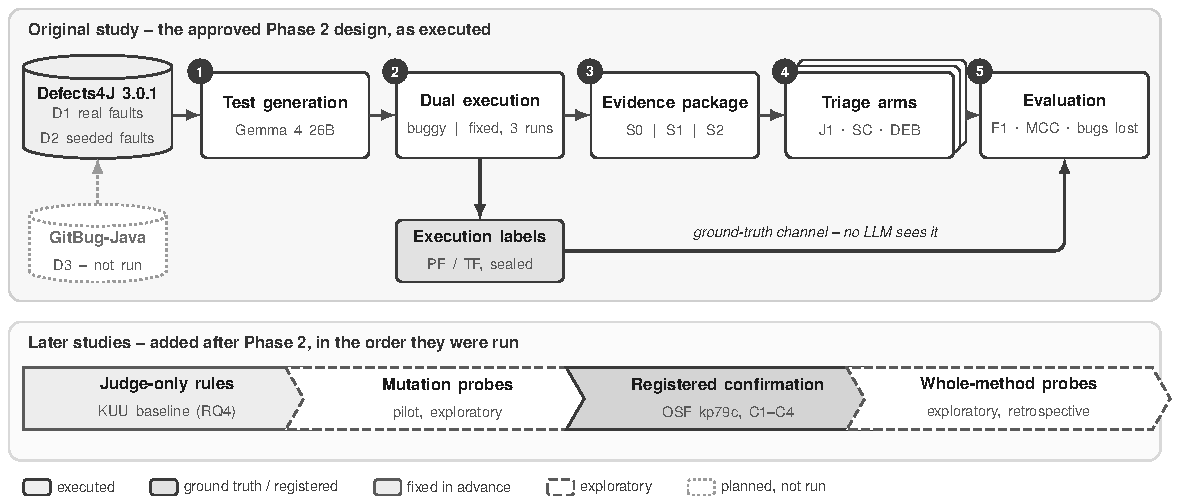
\includegraphics[width=\textwidth]{figures/fig_final_architecture.pdf}
\caption{Research architecture as implemented. Solid blue: the approved Phase~2 design, executed. Green: the ground-truth channel, which bypasses every LLM. Dashed violet: investigations added after the Phase~2 design. Dotted grey: planned in Phase~2 and not run. The editable source is \texttt{figures/fig\_final\_architecture.drawio}.}\label{fig:arch}
\end{figure*}

\subsection{Ground truth}
Each generated test method is compiled against both versions and executed three times on each, every run in a fresh JVM with a 30\,s timeout. The failure signature $\sigma(t,V)$ is the triple of outcome type, exception class and the test line where the failure surfaced; an outcome is deterministic when all three runs share $\sigma$. A test that fails on $P_B$ and passes on $P_F$ is labelled \PF{} (positive class); one that fails on both with $\sigma_B=\sigma_F$ is \TF; one that fails on both with $\sigma_B\neq\sigma_F$ is AMB and is used only in a sensitivity analysis; non-deterministic, timed-out, environment and non-compiling outcomes are excluded. Labels are computed before any judge runs and are stored where no judging module can read them. Because Defects4J fixes are minimised, the fixed version serves as an operational reference for intended behaviour~\cite{zhao2026misguidance}, not as proof of correctness.



\subsection{Evidence package and specification levels}
The context builder produces a fixed-format package whose items carry identifiers that outputs must cite: test lines $[T_i]$, failure items $[F_1]$ (outcome and exception), $[F_2]$ (message with expected and actual values), $[F_3]$ (failing test line) and $[F_{4\ldots}]$ (normalised stack frames), interface items $[\mathit{Sig}_i]$, Javadoc $[\mathit{Doc}_i]$ and specification fields $[\mathit{Spec}_i]$. The levels are nested: S0 $=[T]+[F]+[\mathit{Sig}]$; S1 adds the Javadoc of $P_B$; S2 adds a specification inferred once per focal method from the signature, Javadoc, call sites and sibling documentation, with lines changed by the fix removed. The focal implementation, the fixed version, the patch, developer tests and bug identifiers are never shown, and a leakage guard blocks any call whose package contains a forbidden string.

\subsection{Triage arms and the proposed debate}
All LLM arms use the same model, decoding parameters and evidence package (Table~\ref{tab:arms}). The framework proposed in Phase~2 is an adversarial debate (DEB, Algorithm~\ref{alg:deb}): a program-fault advocate and a test-fault advocate argue independently in Round~1, each rebuts the other in Round~2, and an adjudicator decides from the four arguments, presented anonymously in a seeded random order, citing evidence identifiers only. Assigning an advocate to the program-fault side is meant to keep bug-revealing tests from being dismissed by a neutral judge that inherits the ``test is wrong'' prior of repair tools. Self-consistency (SC) takes the majority of five samples of the one-shot prompt; SC-T matches debate's consumed tokens.

\begin{table}[t]
\caption{Baselines and LLM arms (calls per instance).}\label{tab:arms}
\footnotesize
\begin{tabularx}{\columnwidth}{@{}l c Y@{}}
\toprule
Arm & Calls & Decision \\
\midrule
DA & 0 & \TF{} for every failure (discard-all, the repair-first practice) \\
KA & 0 & \PF{} for every failure (keep-all) \\
R0 & 0 & \PF{} iff not an assertion failure and the deepest project frame is in main code \\
J1 & 1 & one neutral judgement \\
SC & 5 & majority of five samples of the J1 prompt (ties \TF) \\
SC-T & $k_T$ & majority of $k_T$ samples; $k_T$ = smallest odd $k$ reaching DEB's consumed tokens on the development split \\
DEB & 5 & adjudicator decision after two rounds of adversarial argument \\
\bottomrule
\end{tabularx}
\end{table}

\begin{algorithm}[t]
\caption{Adversarial debate (DEB) for one instance}\label{alg:deb}
\begin{algorithmic}[1]
\Require evidence package $x$, replicate $r$
\State $a_P^{(1)} \gets \mathrm{LLM}(\textsc{AdvP}(x))$; $a_T^{(1)} \gets \mathrm{LLM}(\textsc{AdvT}(x))$ \Comment{independent}
\State $a_P^{(2)} \gets \mathrm{LLM}(\textsc{Rebut}(x, a_P^{(1)}, a_T^{(1)}))$
\State $a_T^{(2)} \gets \mathrm{LLM}(\textsc{Rebut}(x, a_T^{(1)}, a_P^{(1)}))$
\State $\pi \gets$ seeded order of the two sides, named ``Analyst X/Y''
\State $d \gets \mathrm{LLM}(\textsc{Adjudicate}(x, \pi))$ \Comment{cited evidence only}
\State \Return label of $d$, or \textsc{invalid} if $d$ fails the JSON schema
\end{algorithmic}
\end{algorithm}

Every arm emits a JSON record with label, reason category, cited evidence identifiers, a short summary and a descriptive confidence. One deterministic repair parse is attempted; outputs that remain invalid are scored as \TF{} in the primary analysis and excluded in a sensitivity analysis.

\subsection{Later additions: judge-only rules and execution probes}\label{sec:probes}
The following components were not part of the approved Phase~2 design; they were added after the RQ1--RQ3 results, and each carries its own evidence status.

\paragraph{Keep-unless-unanimous (KUU) and escalation (RQ4).} One J1 vote is taken from each of three model families (M1, M2 and a third judge M3); a test is discarded only if all three call it a test fault, and is kept otherwise, including when any answer is invalid. Multi-judge voting and unanimity are established patterns~\cite{wang2025json,becker2026jit,zhang2026testagent}, so KUU is treated as a \emph{baseline}, not as a method. A two-tier cascade sends any disagreement to a frontier judge's debate.

\paragraph{Counterfactual program probes (RQ5, RQ6).} For a test $t$ that fails on $P_B$ with focal method $m$, the engine compiles up to \V{cfz:parameters:max_mutants_per_focal} first-order mutants of $m$ and its same-class callees (operators ROR, AOR, COR, LVR, NEG, STD), runs $t$ on each in a fresh JVM, and classifies each run as FLIP (the test passes, and passes again on a re-run), SHIFT (it fails differently), SAME or ERR. A test has a \emph{flip} if some mutant flips it, and is \emph{decoupled} if at least \V{cfz:parameters:min_compiled_mutants_for_decoupling} mutants compiled and none flipped or shifted it. Two certificates act on a base rule: the keep certificate (CK) keeps a test whose flip breaks no passing sibling test, and the decoupled-discard certificate (CD) discards a decoupled test. The engine reads only the buggy version; it has no code path to the fixed version, labels or developer tests.

\paragraph{Whole-method dependence probes (WDP).} The method body is replaced by one that records entry and throws, and by fixed-return bodies as in pseudo-tested-method detection~\cite{niedermayr2016will,vera2018pseudo}. Level U, ``no entry observed and throw-invariant'', is an operational entry check, not proof that a test cannot reach the method and not evidence of a mutation effect. The rule KUU + CD-U discards level-U failures beside KUU.

\subsection{Changes from the Phase 2 design}\label{sec:changes}
Table~\ref{tab:changes} lists every change between the approved design and the executed study, with its reason and decision record (\texttt{docs/tracking/DECISIONS.md}). No research question, hypothesis, confirmatory endpoint or decision rule of the approved design was changed. The instructor gave no comments on the Phase~2 presentation, so no change was made in response to feedback; every change in Table~\ref{tab:changes} has a technical or design reason.

\begin{table*}[t]
\caption{Changes between the approved Phase~2 design and the executed study. [T] technical or resource constraint; [A] authors' decision before the affected data existed; [S] later scientific extension.}\label{tab:changes}
\scriptsize\setlength{\tabcolsep}{3pt}
\begin{tabularx}{\textwidth}{@{}>{\raggedright\arraybackslash}p{3.3cm} >{\raggedright\arraybackslash}p{4.2cm} Y >{\raggedright\arraybackslash}p{1.6cm}@{}}
\toprule
Phase 2 plan & Executed & Reason and consequence & Record \\
\midrule
API-served judges (DeepSeek-V3, Qwen3 families) and GPT-4.1 generator & local open-weight models: G Gemma~4 26B, M1 Qwen3.5 9B, M2 Gemma~4 12B & [A/T] zero API spend; smaller judges, so results describe locally deployable models; M2 shares G's family & D-21, D-57 \\
Zhao et al.'s frame: 318 methods / 233 defects & frame reconstructed by re-running their selection rule: \V{split:frame_methods} / \V{split:frame_bugs} & [T] the final list is not distributed; same population definition, different count & X-03 \\
Docker image with digest & WSL2 Ubuntu 22.04 with a recorded environment manifest & [T] Docker unavailable; reproducibility rests on the manifest & X-04 \\
D3 GitBug-Java (E5-R2) & not run & [T] build reproduction requires Docker; its 2023 bugs predate the models' training cutoffs & X-05, D-103 \\
E5-R4 prompt paraphrases & not run & [T] dropped with Tier~3 for time; only the second-judge part of Tier~3 was restored; no prompt-sensitivity claim is made & D-59, D-61 \\
S2 leakage audit of 60 inferred specifications & not carried out & lines changed by the fix are removed mechanically; whether an S2 text restates the fixed behaviour was not audited & -- \\
Label audit of 100 instances (50 \PF, 50 \TF) & \V{aud:n_items} instances (all \V{aud:labels:PF} development \PF) & [T] the development split holds only \V{aud:labels:PF} \PF{} instances & D-82, D-108 \\
Development gate: J1 F1 above both trivial baselines & M1 failed (F1 \V{devgate:G_d_detail:J1_f1} vs R0 \V{devgate:G_d_detail:R0_f1}); kept under the fixed fallback ladder & [A] no pipeline defect found; nulls describe a judge below its own gate & D-48--D-52 \\
1:2 \PF{}:\TF{} sample ``stratified by project'' & ratio applied over the split, project-stratified & [A] wording ambiguous; reading fixed before held-out data & D-53 \\
GLMM with lme4 & statsmodels with bug-level bootstrap intervals & [T] R unavailable; exploratory only & X-02, X-06 \\
-- & RQ4 rules, probes, registered confirmation, WDP & [S] added after RQ1--RQ3; status in Table~\ref{tab:status} & D-95--D-152 \\
\bottomrule
\end{tabularx}
\end{table*}

%% =====================================================================================
\section{Experimental Setup}\label{sec:setup}

\paragraph{Data and splits.} D1 uses Defects4J~3.0.1~\cite{just2014defects4j,defects4j301}, available at \url{https://github.com/rjust/defects4j} (tag v3.0.1). The frame follows Zhao et al.~\cite{zhao2026misguidance}: fix-changed public or protected methods present in both versions and invoked by a bug-triggering developer test. Re-running their selection rule with their replication package~\cite{zhao2026replication} screened \V{split:candidates} candidates and kept \V{split:frame_methods} methods from \V{split:frame_bugs} defects; a per-project cap of \V{split:per_project:Lang:sampled} left \V{split:sampled_methods} methods from \V{split:sampled_bugs} defects. Before any test was generated, a seeded draw placed three projects (\V{der:dev methods} methods) in the development split and \V{der:n test projects} projects (\V{der:test methods} methods) in the held-out split; every prompt and threshold was chosen on the development split only. D2, a contamination control, applies one killed mutant inside a held-out focal method of the fixed version. Table~\ref{tab:flow} gives the population flow.

\begin{table}[t]
\caption{Population flow. Executed: generated test methods run on both versions; scored: \PF{} and \TF{} instances used at S1 after leakage aborts (D1, D2) or as registered (confirmation).}\label{tab:flow}
\footnotesize\setlength{\tabcolsep}{2.5pt}
\begin{tabular}{@{}l r r r r r@{}}
\toprule
Set & Labelled & \PF & \TF & AMB & Scored \\
\midrule
D1 (both splits) & \multicolumn{5}{l}{\V{ds1:executed_methods} executed: \V{ds1:exclusions:PASS} pass on $P_B$, \V{ds1:exclusions:NC} NC} \\
D1-test & -- & \V{der:d1 test PF labelled} & \V{der:d1 test TF labelled} & \V{der:d1 test AMB labelled} & \V{sum:leakage_abort_exclusions:n_per_level:S1} \\
D2 & \V{d2rep:before_cap:d2_units_total} mut. & \V{d2rep:before_cap:labelled_instances:PF} & \V{d2rep:before_cap:labelled_instances:TF} & \V{d2rep:before_cap:labelled_instances:AMB} & \V{d2:DEB|S1:n_instances} \\
Conf.\ F1 & \V{dsf1:instances} & \V{dsf1:labels:PF} & \V{dsf1:labels:TF} & \V{dsf1:labels:AMB} & -- \\
Conf.\ F2 & \V{dsf2:instances} & \V{dsf2:labels:PF} & \V{dsf2:labels:TF} & \V{dsf2:labels:AMB} & -- \\
Conf.\ CTRL & \V{dsct:instances} & \V{cc:control:PF} & \V{dsct:labels:TF} & -- & control \\
\bottomrule
\end{tabular}
\end{table}

\paragraph{Generation, labels and sampling.} The generator wrote three generations per focal method from the buggy context (temperature 0.7). All \PF{} instances were kept and \TF{} instances sampled, stratified by project, to twice the \PF{} count, with inverse-probability weights for precision at the natural prevalence. The judged D1-test sample has \V{sum:prevalence:judged_sample_prevalence_by_dataset:D1:PF} \PF{} (in \V{pil:scored:bugs_with_PF} bugs), \V{sum:prevalence:judged_sample_prevalence_by_dataset:D1:TF} \TF{} and \V{sum:prevalence:judged_sample_prevalence_by_dataset:D1:AMB} AMB instances; \V{sum:leakage_abort_exclusions:counts_labelled:S1|full:instances} leakage-guard aborts at S1 leave \V{sum:leakage_abort_exclusions:n_per_level:S1} scored instances (\PF{} prevalence \V{sum:prevalence:pf_prevalence}); D2 has \V{d2:DEB|S1:n_instances} (prevalence \V{sum2:prevalence:pf_prevalence}).

\paragraph{Models and hyperparameters.} All models were open-weight and served by Ollama~\V{frozen:runtime:version}~\cite{ollama04013} on one laptop GPU (\V{frozen:hardware:name}, \V{frozen:hardware:mem_total_mib@0}\,MiB; \V{frozen:hardware:ram_total_gib@0}\,GB RAM). G is Gemma~4 26B-A4B~\cite{gemma4} (\texttt{\V{frozen:roles:G}}, Q4\_K\_M); M1 is Qwen3.5 9B~\cite{qwen35_9b} (\texttt{\V{frozen:roles:M1}}); M2 is Gemma~4 12B (\texttt{\V{frozen:roles:M2}}); M3 is Ministral~3 14B. Judge calls used temperature \V{frozen:frozen_models:M1:temperature:judges@1}, top-$p$ \V{frozen:frozen_models:M1:top_p@1}, context \V{frozen:frozen_models:M1:num_ctx@int}, at most \V{frozen:frozen_models:M1:num_predict:judge_roles} output tokens, a per-call seed and thinking disabled; the specification inferencer used temperature \V{frozen:frozen_models:M1:temperature:spec_inferencer@0}; $k_T=\V{frozen:decoding:k_T}$. Prompts (five rounds on the development split), runtime, digests and decoding were frozen in one file before any held-out call. Executions used Ubuntu~22.04.5 under WSL2 with OpenJDK~11; analysis used Python, SciPy and statsmodels~\cite{seabold2010statsmodels}.

\paragraph{Experiments.} E1--E3 run every arm at S0--S2 with M1 on D1-test, \V{frozen:decoding:replicates} replicates (SC-T at S1); E4 (ablations A1--A5) and E5 (D2 with M1; M2 on D1-test and D2) use one replicate. Further judges, including a frontier reference (Claude Sonnet~5.5), are in Supplementary Appendix~\Sref{app:post}. The confirmation used bugs the original study never generated for, in frame F1 (the original frame's methods of unseen bugs), frame F2 (fix-changed methods that no bug-triggering test calls by name) and a control group CTRL (one unchanged method per bug in the same class); labels and probe ledgers were committed before the judge votes and the analysis.

\paragraph{Statistics.} Metrics are computed per replicate and averaged. 95\% confidence intervals come from a 10{,}000-resample bug-level cluster bootstrap~\cite{efron1993bootstrap} with identical resamples for paired differences; a bootstrap $p$ is two-sided. The five confirmatory F1 tests (H1: J1 vs R0; H2a: S1 vs S0 on methods with Javadoc; H2b: S2 vs S1; H3a: DEB vs SC; H3b: SC vs J1) are Holm-corrected~\cite{holm1979}, with recall and precision as a secondary family; equivalence is declared when the 90\% CI lies within $\pm0.05$ F1~\cite{lakens2017equivalence}. The registered family C1--C4 is a separate Holm family at $\alpha=0.05$ (\V{cc:resamples} resamples, seed \V{cc:seed@id}). The bug-loss rate carries an exact one-sided 95\% upper bound. Table~\ref{tab:status} gives the evidence status of every result; a hypothesis ``fixed in advance'' was written into the version-controlled decision log before its calls, which is internal provenance, not an external preregistration.

\begin{table}[t]
\caption{Evidence status of each kind of result.}\label{tab:status}
\footnotesize
\begin{tabularx}{\columnwidth}{@{}>{\raggedright\arraybackslash}p{2.6cm} Y@{}}
\toprule
Result & Status \\
\midrule
RQ1--RQ3 (H1--H3b) & confirmatory family of the approved design; protocol frozen before held-out calls (internal provenance) \\
E4, E5 & exploratory / robustness \\
RQ4 (KUU, cascade) & fixed in advance in the decision log on D2; post hoc on D1; KUU is a baseline \\
Probe pilot & exploratory (labels known) \\
C1--C4, rules, control & confirmatory, registered (OSF \V{osf:osf_id}) \\
WDP & exploratory; retrospective; protocol frozen internally in Git before the runs; not externally preregistered; designed after the confirmation outcomes were known \\
\bottomrule
\end{tabularx}
\end{table}

%% =====================================================================================
\section{Results and Analysis}\label{sec:results}

\subsection{RQ1: triage accuracy against ground truth (E1)}
Table~\ref{tab:e1} reports every arm at S1. Keep-all reaches F1 \V{d1:KA:f1} with MCC \V{d1:KA:mcc}, so F1 alone would rank a constant answer level with the best LLM arm. Every LLM arm has a positive MCC and R0 a negative one (\V{d1:R0:mcc}). DEB has the highest F1 (\V{d1:DEB|S1:f1}) and MCC (\V{d1:DEB|S1:mcc}, interval excluding zero), but exceeds keep-all's F1 by only \V{der:d1 DEB-KA f1}, and it discards \V{d1:DEB|S1:pf_lost@0} of the \V{sum:prevalence:PF} bug-revealing tests per replicate (SC \V{d1:SC|S1:pf_lost@0}, R0 \V{d1:R0:pf_lost@0}, discard-all \V{d1:DA:pf_lost@0}). At the natural prevalence its precision is \V{d1:DEB|S1:precision_prev_adj}. H1 (J1 vs R0) gives $\Delta$F1 \V{conf:f1:H1:delta} (\V{conf:f1:H1:ci95}, $p_\mathrm{Holm}$ \V{conf:f1:H1:p_holm}): inconclusive.

\begin{table}[t]
\caption{E1 at S1, D1-test, judge M1 (mean of \V{frozen:decoding:replicates} replicates). $P_\mathrm{adj}$: precision at the natural prevalence; Lost: \PF{} tests classified \TF{} (of \V{sum:prevalence:PF}).}\label{tab:e1}
\footnotesize\setlength{\tabcolsep}{2pt}
\begin{tabular}{@{}l c c c c c c@{}}
\toprule
Arm & F1 & MCC [95\% CI] & P & R & $P_\mathrm{adj}$ & Lost \\
\midrule
DA & \V{d1:DA:f1} & \V{d1:DA:mcc} & n/a & \V{d1:DA:recall} & n/a & \V{d1:DA:pf_lost} \\
KA & \V{d1:KA:f1} & \V{d1:KA:mcc} & \V{d1:KA:precision} & \V{d1:KA:recall} & \V{d1:KA:precision_prev_adj} & \V{d1:KA:pf_lost} \\
R0 & \V{d1:R0:f1} & \V{d1:R0:mcc} \V{d1:R0:mcc_ci95} & \V{d1:R0:precision} & \V{d1:R0:recall} & \V{d1:R0:precision_prev_adj} & \V{d1:R0:pf_lost} \\
J1 & \V{d1:J1|S1:f1} & \V{d1:J1|S1:mcc} \V{d1:J1|S1:mcc_ci95} & \V{d1:J1|S1:precision} & \V{d1:J1|S1:recall} & \V{d1:J1|S1:precision_prev_adj} & \V{d1:J1|S1:pf_lost@1} \\
SC & \V{d1:SC|S1:f1} & \V{d1:SC|S1:mcc} \V{d1:SC|S1:mcc_ci95} & \V{d1:SC|S1:precision} & \V{d1:SC|S1:recall} & \V{d1:SC|S1:precision_prev_adj} & \V{d1:SC|S1:pf_lost@1} \\
SC-T & \V{d1:SC-T|S1:f1} & \V{d1:SC-T|S1:mcc} \V{d1:SC-T|S1:mcc_ci95} & \V{d1:SC-T|S1:precision} & \V{d1:SC-T|S1:recall} & \V{d1:SC-T|S1:precision_prev_adj} & \V{d1:SC-T|S1:pf_lost@1} \\
DEB & \V{d1:DEB|S1:f1} & \V{d1:DEB|S1:mcc} \V{d1:DEB|S1:mcc_ci95} & \V{d1:DEB|S1:precision} & \V{d1:DEB|S1:recall} & \V{d1:DEB|S1:precision_prev_adj} & \V{d1:DEB|S1:pf_lost@1} \\
\bottomrule
\end{tabular}
\end{table}

\subsection{RQ2 and RQ3: specification and equal budget (E2, E3)}
No arm improved from S0 to S1: Javadoc changed F1 by \V{der:d1 J1 S1-S0 f1} (J1), \V{der:d1 SC S1-S0 f1} (SC) and \V{der:d1 DEB S1-S0 f1} (DEB). On methods with Javadoc, H2a gives $\Delta$F1 \V{conf:f1:H2a:delta} (\V{conf:f1:H2a:ci95}), significant before correction ($p$ \V{conf:f1:H2a:p}) but not after ($p_\mathrm{Holm}$ \V{conf:f1:H2a:p_holm}). The inferred specification did not help either: H2b gives \V{conf:f1:H2b:delta} (\V{conf:f1:H2b:ci95}, $p_\mathrm{Holm}$ \V{conf:f1:H2b:p_holm}), and its precision difference is practically equivalent to zero (90\% CI \V{conf:secondary:H2b~precision:ci90}). At equal allocated budget, DEB's F1 exceeds SC's by \V{conf:f1:H3a:delta} (H3a, \V{conf:f1:H3a:ci95}, $p_\mathrm{Holm}$ \V{conf:f1:H3a:p_holm}) and SC-T's by \V{sum:sc_t_check:delta}, and SC differs from J1 by \V{conf:f1:H3b:delta} (H3b, $p_\mathrm{Holm}$ \V{conf:f1:H3b:p_holm}). DEB consumed \V{d1:DEB|S1:consumed_tokens_per_instance@0} tokens per instance against SC's \V{d1:SC|S1:consumed_tokens_per_instance@0} but took \V{d1:DEB|S1:latency_s_per_instance@1}\,s against \V{d1:SC|S1:latency_s_per_instance@1}\,s, because its calls are sequential; its adjudicator sided with the analyst presented last in \V{d1:DEB|S1:position_bias_rate@pct} of decisions. No hypothesis of the confirmatory family is supported after Holm correction, and none is shown to be practically equivalent; all five are inconclusive (forest plot and full table in Supplementary Appendix~\Sref{app:extra}).

\subsection{Robustness (E5)}\label{sec:robust}
On D2, prevalence is higher (keep-all F1 \V{d2:KA:f1}, MCC \V{d2:KA:mcc}), so only MCC and the mix-free rates compare across datasets. Every M1 arm again has a positive MCC and beats R0 (\V{d2:R0:mcc}); DEB has the highest MCC (\V{d2:DEB|S1:mcc}). M2 improved on M1 in every arm and dataset (DEB on D1-test by \V{r3:D1:m2_minus_m1:DEB:f1:delta}, \V{r3:D1:m2_minus_m1:DEB:f1:ci95}), but shares the generator's family. M1's DEB varied by \V{rn:noise:DEB:f1:range} F1 across replicates. D3 and the prompt paraphrases were not run (Table~\ref{tab:changes}).

\subsection{RQ4: judge-only rules and the KUU baseline}
Figure~\ref{fig:rates} places every rule on two rates that do not depend on the \PF{}:\TF{} mix. Single-judge arms discard about half of the bug-revealing tests, while the cross-family vote lost far fewer. KUU was defined after the D1 vote and tested once on D2 with hypotheses fixed in advance: on D2 it lost \V{kuu2:summary:KUU|S1:pf_lost@0} of \V{kuu2:pf_prevalence:PF} bug-revealing tests against DEB's \V{kuu2:summary:DEB|S1:pf_lost@0} ($p_\mathrm{Holm}$ \V{kuu2:hypotheses:H10-2:p_holm}) and its F1 (\V{kuu2:summary:KUU|S1:f1}) exceeded keep-all's (\V{kuu2:summary:KA:f1}, $p_\mathrm{Holm}$ \V{kuu2:hypotheses:H10-1:p_holm}), but its MCC (\V{kuu2:summary:KUU|S1:mcc}) is below DEB's (\V{kuu2:summary:DEB|S1:mcc}) and its balanced accuracy (\V{rv11:D2:rules:KUU|S1:ba}) below debate's (\V{rv11:D2:rules:DEB|S1:ba}). KUU is therefore a conservative operating point, not a better classifier. A variant without the generator-family judge (KUU-NG) lost \V{kuung:D2:summary:KUUNG|S1:pf_lost@0} bug-revealing test and no bug on D2; escalating disagreements to a frontier judge raised MCC to \V{cas2:summary:CAS|S1:mcc}, without showing non-inferiority to that judge alone (Supplementary Appendix~\Sref{app:cascade}).

\begin{figure*}[t]
\centering
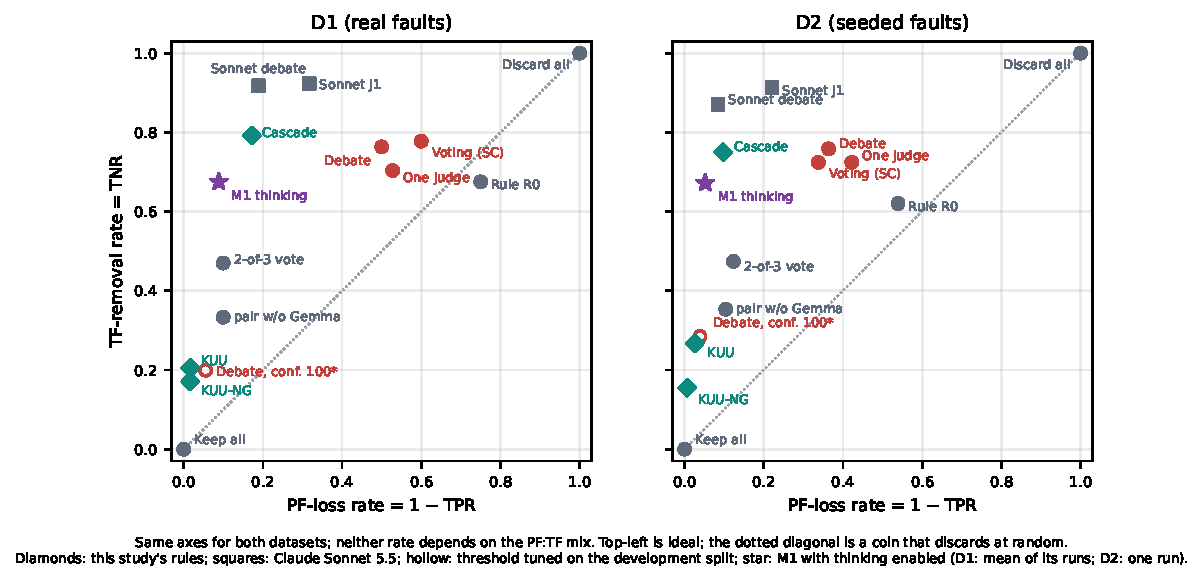
\includegraphics[width=0.78\textwidth]{figures/fig_tradeoff_rates.pdf}
\caption{Every rule on mix-independent rates (post hoc, descriptive): \PF-loss rate ($1-$TPR) against \TF-removal rate (TNR) on D1-test and D2; top left is best. Diamonds: this study's rules; squares: the frontier judge; hollow: the one threshold tuned on the development split; star: M1 with thinking enabled.}\label{fig:rates}
\end{figure*}

\subsection{From an exploratory pilot to a registered confirmation}\label{sec:confirm}
On the D1-test split (\V{pil:scored:PF} \PF{} and \V{pil:scored:TF} \TF{} tests, \V{pil:scored:bugs_with_PF} bugs with a bug-revealing test), a flip occurred for \V{pil:flags:flip:rate_PF} of bug-revealing tests and \V{pil:flags:flip:rate_TF} of wrong tests (difference \V{pil:flags:flip:diff_PF_minus_TF@signed}, \V{pil:flags:flip:diff_ci95}), and \V{pil:flags:decoupled:TF_flagged} of \V{pil:flags:decoupled:n_flagged} decoupled tests were wrong. These estimates are exploratory: the labels were known when the rules were written, the sample was small, and one design amendment (callee mutants) followed the first look. The claim was therefore registered on OSF (\V{osf:osf_id}, \V{osf:registered_utc}) before any confirmation test was generated, with C1 (flip rate among \PF{} minus among \TF), C2 (decoupled rate among \TF{} minus among \PF), C3 (balanced accuracy of KUU + CD minus KUU) and C4 (\PF{} tests lost by 2-of-3 + CK minus 2-of-3) as one Holm family.

\paragraph{Population.} The confirmation scored \V{cc:population:instances} failing tests (\V{cc:population:PF} \PF, \V{cc:population:TF} \TF) from \V{cc:population:bugs} bugs, of which only \V{cc:population:bugs_with_PF} carry a bug-revealing test, below the registered planning range of \V{atx:plan lo}--\V{atx:plan hi}; the registered readings were applied unchanged.

\begin{table}[t]
\caption{The registered family, printed as registered (one Holm family, $\alpha=0.05$; bug-level bootstrap). C1, C2: rate differences; C3: balanced accuracy, KUU + CD minus KUU; C4: \PF{} tests lost, 2-of-3 + CK minus 2-of-3.}\label{tab:family}
\scriptsize\setlength{\tabcolsep}{1.6pt}
\begin{tabular}{@{}l r l r l@{}}
\toprule
 & Estimate & 95\% CI & $p_\mathrm{Holm}$ & Registered reading \\
\midrule
C1 & \V{cc:family:C1:difference@signed} & \V{cc:family:C1:ci95} & \V{cc:family:C1:p_holm@4} & not supp.\textsuperscript{a} \\
C2 & \V{cc:family:C2:difference@signed} & \V{cc:family:C2:ci95} & \V{cc:family:C2:p_holm@4} & supported \\
C3 & \V{cc:family:C3:difference@signed} & \V{cc:family:C3:ci95} & \V{cc:family:C3:p_holm@4} & inconcl.\textsuperscript{b} \\
C4 & \V{cc:family:C4:difference@signed} & \V{cc:family:C4:ci95} & \V{cc:family:C4:p_holm@4} & inconcl.\textsuperscript{b} \\
\bottomrule
\end{tabular}
\par\smallskip\noindent\scriptsize Not supp.: not supported; inconcl.: inconclusive. \textsuperscript{a}powered by the registered planning, so it counts against the method, with the sample-size qualifier; \textsuperscript{b}underpowered by the registered planning.
\end{table}

\paragraph{C1: the flip did not replicate.} The flip rate was \V{dv:flip rate pf@3} for bug-revealing tests (\V{cc:family:C1:PF_flagged} of \V{cc:family:C1:PF}) and \V{dv:flip rate tf@3} for wrong tests (\V{cc:family:C1:TF_flagged} of \V{cc:family:C1:TF}) (Table~\ref{tab:family}, Figure~\ref{fig:confirm}). The interval excludes the pilot's estimate but includes half of it, so a small positive effect is not excluded. The flip rate among control failures, \V{cc:control:flip_rate_TF@3}, lies with both: a single edit makes a failing generated test pass about equally often whichever side is at fault.

\paragraph{C2: decoupling held, with limits.} In the pooled analysis, \V{cc:family:C2:TF_flagged} of the \V{dv:dec flagged} decoupled tests are wrong (Holm $p$ \V{cc:family:C2:p_holm@4}). The registered per-frame analysis gives \V{cf1:family:C2:difference@signed} \V{cf1:family:C2:ci95@ci2} in F1 and \V{cf2:family:C2:difference@signed} \V{cf2:family:C2:ci95@ci2} in F2, so the effect is not reproduced in F1; \V{arow:jackson dec tf} of the \V{cc:family:C2:TF_flagged} decoupled wrong tests lie in two projects (JacksonDatabind, JacksonCore), and without them the estimate is \V{atx:noJ est@signed} \V{atx:noJ ci} (exploratory).

\begin{figure*}[t]
\centering
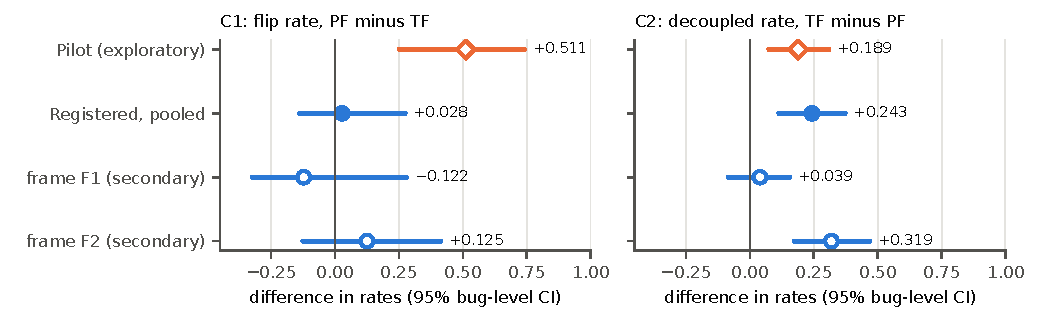
\includegraphics[width=0.74\textwidth]{figures/fig_final_confirmation.pdf}
\caption{Pilot (exploratory, D1-test, labels known) beside the registered confirmation (OSF \V{osf:osf_id}) and its registered per-frame secondary analyses. Points: rate differences; bars: 95\% bug-level bootstrap intervals. Data: \texttt{figures/fig\_final\_confirmation\_data.csv}.}\label{fig:confirm}
\end{figure*}

\paragraph{C3, C4 and the rules.} C3 ($p_\mathrm{Holm}$ \V{cc:family:C3:p_holm@4}) and C4 ($p_\mathrm{Holm}$ \V{cc:family:C4:p_holm@4}) are inconclusive. Table~\ref{tab:rules} leads with TPR, TNR and bugs lost, since balanced accuracy hides a lost bug: adding CD to KUU raised TNR by \V{dv:kuu cd dtnr@3} and lost one bug (\texttt{Math\_59}), and the keep certificate's evidence was set for \V{cc:secondary:rcf_in_place_of_flip:PF_flagged} of \V{cc:population:PF} bug-revealing and \V{cc:secondary:rcf_in_place_of_flip:TF_flagged} of \V{cc:population:TF} wrong tests, so it has no support here. Control failures (\V{cc:control:instances}, from \V{cc:control:bugs} bugs) are on methods the fix did not change, which are not known to be defect-free.

\begin{table}[t]
\caption{Rules on the \V{cc:rules:instances_with_three_votes} confirmation tests with three judge votes (\V{cc:rules:PF} \PF; reported, not tested except through C3 and C4). Bound: exact one-sided 95\% upper bound on the bug-loss rate.}\label{tab:rules}
\footnotesize\setlength{\tabcolsep}{2.5pt}
\begin{tabular}{@{}l r r r r r@{}}
\toprule
Rule & TPR & TNR & Lost & Bugs lost & Bound \\
\midrule
KUU & \V{cc:rules:KUU:TPR@3} & \V{cc:rules:KUU:TNR@3} & \V{cc:rules:KUU:PF_lost} & \V{cc:rules:KUU:bugs_lost}/\V{cc:rules:KUU:bugs_with_PF} & \V{cc:rules:KUU:upper95_bug_loss_rate@3} \\
KUU + CD & \V{cc:rules:KUU+CD:TPR@3} & \V{cc:rules:KUU+CD:TNR@3} & \V{cc:rules:KUU+CD:PF_lost} & \V{cc:rules:KUU+CD:bugs_lost}/\V{cc:rules:KUU+CD:bugs_with_PF} & \V{cc:rules:KUU+CD:upper95_bug_loss_rate@3} \\
2-of-3 & \V{cc:rules:2-of-3:TPR@3} & \V{cc:rules:2-of-3:TNR@3} & \V{cc:rules:2-of-3:PF_lost} & \V{cc:rules:2-of-3:bugs_lost}/\V{cc:rules:2-of-3:bugs_with_PF} & \V{cc:rules:2-of-3:upper95_bug_loss_rate@3} \\
2-of-3 + CK & \V{cc:rules:2-of-3+CK:TPR@3} & \V{cc:rules:2-of-3+CK:TNR@3} & \V{cc:rules:2-of-3+CK:PF_lost} & \V{cc:rules:2-of-3+CK:bugs_lost}/\V{cc:rules:2-of-3+CK:bugs_with_PF} & \V{cc:rules:2-of-3+CK:upper95_bug_loss_rate@3} \\
keep-all + CD & \V{cc:rules:keep-all+CD:TPR@3} & \V{cc:rules:keep-all+CD:TNR@3} & \V{cc:rules:keep-all+CD:PF_lost} & \V{cc:rules:keep-all+CD:bugs_lost}/\V{cc:rules:keep-all+CD:bugs_with_PF} & \V{cc:rules:keep-all+CD:upper95_bug_loss_rate@3} \\
\bottomrule
\end{tabular}
\end{table}

\subsection{What the surviving signal is (exploratory)}\label{sec:surviving}
Everything in this subsection was chosen after the confirmation outcomes were known; the independent audit of the registered analysis recomputed every registered quantity from raw records and found no discrepancy (Supplementary Appendix~\Sref{app:registration}). Decoupling fired where an exception is raised outside the method under test, mostly in F2. Both lost bugs are faults that none of the six operators can touch: \texttt{Math\_59}, the confirmation's one decoupled bug-revealing test, had exactly \V{arow:math59 ncomp} compiled mutants, all silent, and the pilot's \texttt{Codec\_13} was a replaced call. The flag therefore conflates ``the failure does not depend on this method'' with ``the edits could not reach what it depends on''.

\paragraph{Whole-method dependence probes (exploratory, retrospective).} \emph{Status: exploratory; retrospective; protocol frozen internally in Git before the runs; not externally preregistered; designed after the confirmation outcomes were known.} On the \V{wdp:populations:CONF-votes:instances} confirmation tests with three votes, discarding level-U failures beside KUU removed \V{wdp:primary:paired:TNR:difference@signed} more wrong tests than KUU (95\% CI \V{wdp:primary:paired:TNR:ci95}) with no bug-revealing test and no bug lost (Table~\ref{tab:wdp}). No bug-revealing test reached level U (\V{wdp:secondary:3_level_U_by_label:CONF-all:U:PF_flagged} of \V{wdp:secondary:3_level_U_by_label:CONF-all:U:PF}; pilot \V{wdp:secondary:3_level_U_by_label:PILOT-all:U:PF_flagged} of \V{wdp:secondary:3_level_U_by_label:PILOT-all:U:PF}), against \V{wdp:secondary:3_level_U_by_label:CONF-all:U:TF_flagged} of \V{wdp:secondary:3_level_U_by_label:CONF-all:U:TF} wrong tests. Over \V{wdp:pooled_bound:bugs_with_PF} bugs with a bug-revealing test, the one-sided 95\% upper bound on additional bug loss is \V{wdp:pooled_bound:upper95@3}; this bound is optimistic, because the rule was designed with knowledge of these bugs. The gain is concentrated: level U flagged \V{wdp:secondary:9_heterogeneity:F2:level_U_by_label:U:TF_flagged} of \V{wdp:secondary:9_heterogeneity:F2:level_U_by_label:U:TF} wrong tests in F2 but \V{wdp:secondary:9_heterogeneity:F1:level_U_by_label:U:TF_flagged} of \V{wdp:secondary:9_heterogeneity:F1:level_U_by_label:U:TF} in F1, and without the two Jackson projects the gain is \V{wdp:secondary:9_heterogeneity:without_Jackson:primary:paired:TNR:difference@signed} \V{wdp:secondary:9_heterogeneity:without_Jackson:primary:paired:TNR:ci95}. Of the \V{wdp:secondary:4_ladder:registered_decoupled:CONF:TF:n} wrong tests the registered certificate flagged, \V{wdp:secondary:4_ladder:registered_decoupled:CONF:TF:U} are level U, so most of the surviving signal is an entry check rather than a mutation effect.

\begin{table}[t]
\caption{WDP on the \V{wdp:populations:CONF-votes:instances} confirmation tests with three votes (\V{wdp:populations:CONF-votes:PF} \PF, \V{wdp:populations:CONF-votes:bugs_with_PF} bugs with one). Exploratory, retrospective, not externally preregistered.}\label{tab:wdp}
\footnotesize
\begin{tabular*}{\columnwidth}{@{\extracolsep{\fill}}lrrrr@{}}
\toprule
Rule & TPR & TNR & Bugs lost & Bound \\
\midrule
KUU & \V{wdp:secondary:6_rules:CONF-votes:KUU:TPR@3} & \V{wdp:secondary:6_rules:CONF-votes:KUU:TNR@3} & \V{wdp:secondary:6_rules:CONF-votes:KUU:bugs_lost} & \V{wdp:secondary:6_rules:CONF-votes:KUU:upper95_bug_loss_rate@3} \\
KUU + CD & \V{wdp:secondary:6_rules:CONF-votes:KUU+CD:TPR@3} & \V{wdp:secondary:6_rules:CONF-votes:KUU+CD:TNR@3} & \V{wdp:secondary:6_rules:CONF-votes:KUU+CD:bugs_lost} & \V{wdp:secondary:6_rules:CONF-votes:KUU+CD:upper95_bug_loss_rate@3} \\
KUU + CD-U & \V{wdp:secondary:6_rules:CONF-votes:KUU+CD-U:TPR@3} & \V{wdp:secondary:6_rules:CONF-votes:KUU+CD-U:TNR@3} & \V{wdp:secondary:6_rules:CONF-votes:KUU+CD-U:bugs_lost} & \V{wdp:secondary:6_rules:CONF-votes:KUU+CD-U:upper95_bug_loss_rate@3} \\
\bottomrule
\end{tabular*}
\end{table}



%% =====================================================================================
\section{Comparison with Base Papers}\label{sec:comparison}

\paragraph{Summary.} Table~\ref{tab:base} lists the base papers with their problem, method, data, metric, reported result and the limitation that matters for triage. All reported results are the original authors' (*).

\begin{table*}[t]
\caption{Base papers. Reported results are taken from the original papers (*).}\label{tab:base}
\scriptsize\setlength{\tabcolsep}{3pt}
\begin{tabularx}{\textwidth}{@{}p{2.3cm} Y Y Y Y@{}}
\toprule
Paper (year) & Problem; method & Data; metric & Reported result (*) & Limitation for triage \\
\midrule
Xie et al., MACO (2026)~\cite{xie2026maco} & generation; cooperating agents with coverage feedback & \V{cit:maco methods} Java methods; line/branch coverage & \V{cit:maco line}\%, \V{cit:maco branch}\%\cited & current code only; budgets not aligned \\
Xu et al., CANDOR (2026)~\cite{xu2026candor} & generation and oracles; consensus panel & HumanEvalJava, LeetCodeJava; oracle correctness & \V{cit:candor lo}--\V{cit:candor hi}\cited & dependency-free methods \\
Liu et al., JSTestCraft (2026)~\cite{liu2026jstestcraft} & generation; context agents, three-LLM triage vote & \V{cit:jstestcraft repos} Node.js repositories; audited recall & triage recall \V{cit:jstestcraft recall}\%\cited & recall from one small audit \\
Gu et al., TestART (2026)~\cite{gu2026testart} & generation with template repair & Defects4J; pass rate & \V{cit:testart pass}\%\cited & rewrites assertions to observed values \\
Hayet et al., ChatAssert (2025)~\cite{hayet2025chatassert} & oracle generation with dynamic repair & TECO data; Acc@1 & +\V{cit:chatassert}\%\cited & match-based; presumes correct code \\
Taherkhani et al., VALTEST (2026)~\cite{taherkhani2026valtest} & test validity from semantic entropy & HumanEval, MBPP, LeetCode; validity & up to +\V{cit:valtest}\%\cited & validity from a reference solution \\
Walczak et al. (2026)~\cite{walczak2026context} & context levels for generation & \V{cit:walczak methods} custom methods; branch coverage & docstrings +\V{cit:walczak docstring} pp\cited & correct code only \\
Li et al., MitGen (2026)~\cite{li2026mitgen} & failing-test generation via reference implementations & EvoEval, ClassEval; failing-test recall & \V{cit:mitgen ours} vs \V{cit:mitgen base}\cited & single-statement faults \\
Yaraghi et al., TaRGET (2025)~\cite{yaraghi2025target} & test repair with fine-tuned code models & TaRBench; exact match & \V{cit:target em}\%\cited & assumes the test is wrong \\
Maddila et al. (2026)~\cite{maddila2026agentic} & agentic program repair after rule-based triage & Meta monorepo; solve rate & \V{cit:maddila solve}\%\cited & triage not evaluated \\
\bottomrule
\end{tabularx}
\end{table*}

\paragraph{Quantitative comparison.} Only JSTestCraft reports a triage metric (an audited recall) and JavaOracle a precision. Table~\ref{tab:quant} lists both, marked *, beside the arms measured here on identical D1-test instances: discard-all re-implements repair-first generators, R0 rule-based triage, VOTE3 a three-family majority vote in JSTestCraft's manner with local judges, and DEB the debate idea of JavaOracle under a fixed budget.

\begin{table}[t]
\caption{Quantitative comparison. Rows marked * are published figures from other settings, not measured here and not comparable; all other rows are measured on the same \V{sum:leakage_abort_exclusions:n_per_level:S1} D1-test instances at S1.}\label{tab:quant}
\footnotesize\setlength{\tabcolsep}{2pt}
\begin{tabular}{@{}l c c c c@{}}
\toprule
Method & P & R & F1 & MCC \\
\midrule
JSTestCraft vote*~\cite{liu2026jstestcraft} & n/r & \V{cit:jstestcraft recall}\%\cited & n/r & n/r \\
JavaOracle debate*~\cite{fu2026javaoracle} & \V{cit:javaoracle precision}\cited & n/r & n/r & n/r \\
\midrule
Discard-all (re-impl.) & n/a & \V{d1:DA:recall} & \V{d1:DA:f1} & \V{d1:DA:mcc} \\
Keep-all (re-impl.) & \V{d1:KA:precision} & \V{d1:KA:recall} & \V{d1:KA:f1} & \V{d1:KA:mcc} \\
Rule-based R0 (re-impl.) & \V{d1:R0:precision} & \V{d1:R0:recall} & \V{d1:R0:f1} & \V{d1:R0:mcc} \\
VOTE3 (re-impl., local) & \V{e8:summary:VOTE3|S1:precision} & \V{e8:summary:VOTE3|S1:recall} & \V{e8:summary:VOTE3|S1:f1} & \V{e8:summary:VOTE3|S1:mcc} \\
SC (this study) & \V{d1:SC|S1:precision} & \V{d1:SC|S1:recall} & \V{d1:SC|S1:f1} & \V{d1:SC|S1:mcc} \\
DEB (this study) & \V{d1:DEB|S1:precision} & \V{d1:DEB|S1:recall} & \V{d1:DEB|S1:f1} & \V{d1:DEB|S1:mcc} \\
\bottomrule
\end{tabular}
\end{table}

\paragraph{Methodological comparison.} Three differences address the base papers' limitations: labels come from execution on buggy and fixed versions rather than audits, reference solutions or assertion matches~\cite{liu2026jstestcraft,taherkhani2026valtest,hayet2025chatassert}, which makes recall and lost tests measurable; specification is manipulated rather than assumed~\cite{xu2026candor,li2026mitgen}; and arms are budget-matched, which MACO, CANDOR and JSTestCraft do not enforce~\cite{xie2026maco,xu2026candor,liu2026jstestcraft}.

\paragraph{Improvement analysis.} On identical instances DEB's F1 exceeds R0's by \V{der:d1 DEB-R0 f1} (relative \V{der:d1 DEB-R0 f1 rel@spct}), SC's by \V{conf:f1:H3a:delta} (\V{der:d1 DEB-SC f1 rel@spct}) and J1's by \V{der:d1 DEB-J1 f1} (\V{der:d1 DEB-J1 f1 rel@spct}), none significantly after Holm; over keep-all the F1 gain is only \V{der:d1 DEB-KA f1} (\V{der:d1 DEB-KA f1 rel@spct}), and the real gain is in MCC (\V{d1:DEB|S1:mcc} vs \V{d1:KA:mcc}). DEB does not outperform keep-all on recall. No improvement over a base paper can be computed, because none reports a triage result on this data, metric or label source.

\paragraph{Fairness and limitations.} The two published figures come from other languages and data, from author audits rather than execution labels, from other prevalences and from much larger models, so they are context, not targets. The re-implemented arms share this study's instances, labels and bootstrap but not the original code (fidelity table in Supplementary Appendix~\Sref{app:extra}). Where the designs meet, results agree: the share of effective generated tests here (\V{zhao:subsets:all_D1:share_effective_pct@2}\%) overlaps Zhao et al.'s range, and a cross-family vote keeps recall high (\V{e8:summary:VOTE3|S1:recall}) as JSTestCraft's does.

%% =====================================================================================
\section{Ablation Study}\label{sec:ablation}
Each ablation changes one component of a full arm and is compared with that parent on identical instances (Table~\ref{tab:abl}; F1, MCC and $p$ per cell in Supplementary Appendix~\Sref{app:extra}). A1 and A2 test whether exchanging arguments and assigning adversarial roles matter, A3 the aggregation threshold, A4 the contribution of execution evidence, and A5 whether the implementation helps or misleads. Debate ablations keep the five-call budget; all are exploratory (one replicate, no multiplicity correction).

\begin{table}[t]
\caption{E4 ablations at S1 (A5b at S2), D1-test, judge M1; $\Delta$F1 = ablated minus parent on identical instances (exploratory, one replicate).}\label{tab:abl}
\scriptsize\setlength{\tabcolsep}{2.5pt}
\begin{tabularx}{\columnwidth}{@{}l Y c c@{}}
\toprule
ID & Change (parent arm) & $\Delta$F1 & 95\% CI \\
\midrule
A1 & no argument exchange (DEB) & \V{abl:A1|S1-DEB|S1:delta} & \V{abl:A1|S1-DEB|S1:ci95} \\
A2 & neutral, not adversarial, debaters (DEB) & \V{abl:A2|S1-DEB|S1:delta} & \V{abl:A2|S1-DEB|S1:ci95} \\
A3 & SC threshold $v\ge2/5$; $v\ge4/5$ (SC) & \multicolumn{2}{c}{F1 \V{sum:A3:SC|S1|A3 v>=2/5:f1}; \V{sum:A3:SC|S1|A3 v>=4/5:f1}} \\
A4 & no failure evidence (J1) & \V{abl:J1|S1|noF-J1|S1:delta} & \V{abl:J1|S1|noF-J1|S1:ci95} \\
A4 & no failure evidence (SC) & \V{abl:SC|S1|noF-SC|S1:delta} & \V{abl:SC|S1|noF-SC|S1:ci95} \\
A4 & no failure evidence (DEB) & \V{abl:DEB|S1|noF-DEB|S1:delta} & \V{abl:DEB|S1|noF-DEB|S1:ci95} \\
A5a & buggy body shown (J1) & \V{abl:J1|S1|impl-J1|S1:delta} & \V{abl:J1|S1|impl-J1|S1:ci95} \\
A5a & buggy body shown (DEB) & \V{abl:DEB|S1|impl-DEB|S1:delta} & \V{abl:DEB|S1|impl-DEB|S1:ci95} \\
A5b & body-derived specification (J1, S2) & \V{abl:J1|S2|specprime-J1|S2:delta} & \V{abl:J1|S2|specprime-J1|S2:ci95} \\
\bottomrule
\end{tabularx}
\end{table}

\textbf{Failure evidence (A4)} is the only component whose removal has a clear effect: F1 drops by \V{abl:SC|S1|noF-SC|S1:delta} for SC and \V{abl:J1|S1|noF-J1|S1:delta} for J1, and their MCC falls to chance (\V{d1:SC|S1|noF:mcc}, \V{d1:J1|S1|noF:mcc}); DEB's F1 also drops, not significantly. The judges' signal therefore comes from the execution evidence, which also argues against decisions recalled from a memorised benchmark. \textbf{Debate components (A1, A2)} do not help: without the exchange or the adversarial roles F1 was slightly higher (\V{abl:A1|S1-DEB|S1:delta}, \V{abl:A2|S1-DEB|S1:delta}), with intervals that include zero, so the debate's small advantage cannot be attributed to adversarial argument. \textbf{Aggregation (A3)}: lowering SC's threshold to two of five votes raised recall to \V{sum:A3:SC|S1|A3 v>=2/5:recall}; requiring four of five cut it to \V{sum:A3:SC|S1|A3 v>=4/5:recall}. \textbf{Implementation (A5)}: showing the buggy body changed F1 by \V{abl:J1|S1|impl-J1|S1:delta} (J1) and \V{abl:DEB|S1|impl-DEB|S1:delta} (DEB), neither significant. No ablation shows that a debate component contributes an improvement.

%% =====================================================================================
\section{Discussion}\label{sec:discussion}

\paragraph{What the measurement shows.} Small thinking-disabled judges carry a weak but real signal (DEB MCC \V{d1:DEB|S1:mcc}) that comes from the failure evidence (A4); neither Javadoc nor an inferred specification helped, and debate was not detectably better than self-consistency at equal budget. These nulls are inconclusive, not evidence of no effect: at 80\% power the detectable F1 difference for DEB versus SC is about \V{mde:tests:H3a:mde_alpha_005@2}, and detecting 0.08 would need about \V{rv18:tests:H3a:by_mde:0.08:bugs_alpha_005} bug clusters rather than \V{rv18:tests:H3a:n0_bugs}. Every local judge failed its own development gate, so the nulls describe weak judges, not the factors in general. With thinking enabled, one M1 call beat M1's debate on D2 ($\Delta$MCC \V{tk:d2:confirmatory:HT-1:delta}, $p_\mathrm{Holm}$ \V{tk:d2:confirmatory:HT-1:p_holm}): for small judges the gain sought in orchestration came from reasoning inside one call, although that judge also failed the gate (Supplementary Appendix~\Sref{app:revision}).

\paragraph{Why the pilot overstated the flip.} The pilot was small, its labels were known when the rules were written, and half of its flipping bug-revealing tests came from one project (Chart) absent from the confirmation. A flip needs an edit that happens to produce the expected value, which real faults rarely allow, while wrong tests are made to pass as easily as right ones. What survived is the negative observable, which concerns dependence on the method, not its correctness.

\paragraph{Practical implications and failure cases.} Triage stages should pass the complete failure (message with expected and actual values, failing line, project frames) to the judge, and should not keep a test because some edit makes it pass. A failure that no edit changes, or that never enters the method under test, is very likely a wrong test, but the check fires unevenly and lost one bug of \V{cc:population:bugs_with_PF} in its registered form. Typical judge errors are accepting a buggy method's rejection as the API contract and misreading a failing \texttt{assertFalse} (Supplementary Table~\Sref{tab:qual}). KUU suits settings where a lost bug costs far more than a false alarm; at 5\% \PF{} prevalence a developer would still read about \V{rv11:D2:rules:KUU|S1:at_prevalence:0.0500:false_alarms_per_kept_pf@0} test faults per bug-revealing test kept.

\paragraph{Were the gaps and objectives met?} G1 (O1, O2), G2 (O3) and G3 (O4) were measured as designed; all five confirmatory effects are inconclusive at this size. O5 was partly met: D2 and a second judge were run, D3 and the paraphrases were not. RQ5: the flip did not replicate, and decoupling held in the pooled registered analysis but not in F1. RQ6: both certificate rules are inconclusive.

\paragraph{Threats to validity.} \textit{Construct:} the fixed version is an operational reference, not proof of correctness, and a test revealing a second real fault is labelled \TF. A blind two-rater audit of \V{aud:n_items} development instances gave $\kappa$ \V{aud2:raters:kappa}~\cite{cohen1960kappa} and \V{aud2:consensus_vs_execution:agreement@pct1} agreement with the execution label, but the raters are the authors and no independent audit of the confirmation's labels exists. Excluding AMB failures matters little (DEB F1 \V{sum:sensitivity_f1:AMB_as_PF:DEB|S1:f1} or \V{sum:sensitivity_f1:AMB_as_TF:DEB|S1:f1} if they are counted). \textit{Internal:} Defects4J is likely in the models' training data~\cite{huang2026ult}; D2 and A4 address recall of fixes, not knowledge of the original code; the S2 leakage audit was not carried out. \textit{Conclusion:} samples are small (\V{sum:prevalence:PF} \PF{} at S1; \V{cc:population:bugs_with_PF} bugs with a bug-revealing test in the confirmation), ablations and E5 have one replicate, bootstrap intervals with few clusters are approximate, projects are not resampled, and non-significance is never read as equivalence. \textit{External:} one benchmark, language and generator, small local judges, no prompt-sensitivity test. \textit{Reporting:} RQ4 and the exploratory analyses followed earlier results; each carries its status (Table~\ref{tab:status}), and the registration's reworded template fields leave the attached frozen bundle as the governing text.

%% =====================================================================================
\section{Conclusion and Future Work}\label{sec:conclusion}

Against buggy/fixed execution labels, small LLM judges with thinking disabled reached F1 \V{d1:DEB|S1:f1} at best against keep-all's \V{d1:KA:f1}, discarded about half of the bug-revealing tests, and none of the approved design's five confirmatory hypotheses was supported or shown equivalent. Judge-only rules lie on one trade-off curve, whose keep-heavy end, KUU, served as the baseline. In a registered confirmation, an edit that makes a failing test pass was not evidence that the test is right, while a failure that no edit changes was a wrong test in \V{cc:family:C2:TF_flagged} of \V{dv:dec flagged} cases, precise where it fires but uneven across frames and projects. Future work should run a fresh registered test of the whole-method dependence check on tests that no probe or judge has seen, add a second generator and an external benchmark, obtain an independent audit of the labels, and compare against a patch-based validator in a setting where an issue report exists.

%% =====================================================================================
\section*{Data and Code Availability}
Defects4J~3.0.1 is public at \url{https://github.com/rjust/defects4j} (tag v3.0.1)~\cite{defects4j301}, and the frame follows the replication package of Zhao et al.~\cite{zhao2026replication}. The implementation, frozen configurations, prompts, analysis scripts, the generated tests, execution labels, evidence packages, parsed judge decisions, probe ledgers, analysis outputs, and the scripts that build every number and figure of this paper are at \url{https://github.com/hafizhuzaifaahmed/llm-failure-triage}. Raw model-call and inference-server logs are not in the public repository because single files exceed its size limit. The confirmation is registered on OSF (\V{osf:osf_id}, \V{osf:registered_utc}); no other part of the study was externally registered.

\section*{Use of AI-Assisted Tools}
Claude Opus~5.5 (Anthropic) was used under the authors' direction to implement the experimental pipeline and its tests, run the experiments and analysis scripts, verify references, build figures and the slide deck, and draft and revise this manuscript; every number in the text is generated from committed analysis outputs. Claude Fable~5.2 (Anthropic) was used read-only to audit the registered confirmation and to write the design and execution brief for the whole-method dependence probes; a Fable~5.2 review of the interpretation of the WDP result was started but stopped at the account's usage limit before producing any output, and the authors waived that review. A separate Claude Opus~5.5 session acted as a sealed third rater in the label audit, reported only as secondary agreement. The open-weight models studied (Qwen3.5, Gemma~4, Ministral~3, Llama~3.1) and Claude Sonnet~5.5 are experimental subjects, not authoring tools. The authors reviewed the code, outcomes, claims and text and take full responsibility for them.

\bibliographystyle{IEEEtran}
\bibliography{references_v2}

\end{document}
